% setup
\documentclass[12pt,a4paper]{article}
%\documentclass[a4paper,12pt]{scrreprt}
\usepackage[left= 2.5cm,right = 2.5cm, bottom = 2.5 cm, top = 2.5cm, head = 14.5pt]{geometry}
\renewcommand{\baselinestretch}{1.5}

\usepackage[utf8]{inputenc}
\usepackage[german]{babel}
\usepackage{csquotes}
\usepackage[T1]{fontenc}
\usepackage{amsmath}
\usepackage{amsfonts}
\usepackage{amssymb}

%matrices and tables
\usepackage{blkarray}
\usepackage{floatrow}
\usepackage{hhline}

%figures & images
\usepackage{graphicx}
\usepackage{subcaption}
\usepackage{float}

%utils
\usepackage{color}
\usepackage{xcolor}
\usepackage{url}
\usepackage[hidelinks]{hyperref}
\usepackage{lipsum}
\usepackage{array}
\usepackage{textcomp}
\usepackage{setspace}
\usepackage{wrapfig}
\usepackage{ragged2e}

%breaklines
%\usepackage{etoolbox}
%\g@addto@macro{\UrlBreaks}{\UrlOrds}
%\def\UrlOrds{\do\*\do\-\do\~\do\'\do\"\do\-}%


%Java und Javascript Code
%\usepackage{listings}
\definecolor{codegray}{rgb}{0.9,0.9,0.9}
\usepackage{minted}
%\usepackage{mdframed}
%
%%\setmintedinline
%\surroundwithmdframed{minted}

%Abkürzugen
\usepackage[acronyms,automake,toc,nopostdot,nomain]{glossaries}
\makeglossaries
\loadglsentries{acronyms}

% Bibliographie
\usepackage[backend=biber,style=alphabetic,citestyle=authoryear]{biblatex}
\bibliography{Thesis}
\usepackage[nottoc]{tocbibind}

\appto\UrlBreaks{\do\a\do\b\do\c\do\d\do\e\do\f\do\g\do\h\do\i\do\j
\do\k\do\l\do\m\do\n\do\o\do\p\do\q\do\r\do\s\do\t\do\u\do\v\do\w
\do\x\do\y\do\z\do\|\do\*\do\-\do\~\do\'\do\"\do\-}

%\renewcounter{biburlnumpenalty}
%\renewcounter{biburlucpenalty}
%\renewcounter{biburllcpenalty}
%
%\newcommand*{\biburlsetup}{%
%  \Urlmuskip=0mu plus 3mu\relax
%  \mathchardef\UrlBigBreakPenalty=100\relax
%  \mathchardef\UrlBreakPenalty=200\relax
%  \def\UrlBigBreaks{\do\:\do\-}%
%  \def\UrlBreaks{%
%    \do\.\do\@\do\/\do\\\do\!\do\_\do\|\do\;\do\>\do\]\do\)\do\}%
%    \do\,\do\?\do\'\do\+\do\=\do\#\do\$\do\&\do\*\do\^\do\"}%
%  \ifnumgreater{\value{biburlnumpenalty}}{0}
%    {\def\do##1{\appto\UrlSpecials{\do##1{\mathchar`##1 \penalty\value{biburlnumpenalty}}}}%
%     \do\1\do\2\do\3\do\4\do\5\do\6\do\7\do\8\do\9\do\0}
%    {}%
%  \ifnumgreater{\value{biburlucpenalty}}{0}
%    {\def\do##1{\appto\UrlSpecials{\do##1{\mathchar`##1 \penalty\value{biburlucpenalty}}}}%
%     \do\A\do\B\do\C\do\D\do\E\do\F\do\G\do\H\do\I\do\J
%     \do\K\do\L\do\M\do\N\do\O\do\P\do\Q\do\R\do\S\do\T
%     \do\U\do\V\do\W\do\X\do\Y\do\Z}
%    {}%
%  \ifnumgreater{\value{biburllcpenalty}}{0}
%    {\def\do##1{\appto\UrlSpecials{\do##1{\mathchar`##1 \penalty\value{biburllcpenalty}}}}%
%     \do\a\do\b\do\c\do\d\do\e\do\f\do\g\do\h\do\i\do\j
%     \do\k\do\l\do\m\do\n\do\o\do\p\do\q\do\r\do\s\do\t
%     \do\u\do\v\do\w\do\x\do\y\do\z}
%    {}%
%  \let\do=\noexpand}

\setcounter{biburlnumpenalty}{8000}
\setcounter{biburlucpenalty}{8000}
\setcounter{biburllcpenalty}{8000}

%\defcounter{biburlnumpenalty}{3000}
%\defcounter{biburlucpenalty}{6000}
%\defcounter{biburllcpenalty}{9000}

% Header Footer
\usepackage[automark,headsepline]{scrlayer-scrpage}
\clearpairofpagestyles
%\pagestyle{fancy}

\lehead{}
\chead{}
\ihead{\slshape}
%
\lefoot{}
\cfoot{}
\rofoot{\thepage}
\pagestyle{scrheadings}

% no indent
%\setlength{\parindent}{0pt}

%fix hyphenation
\usepackage[htt]{hyphenat}
\hyphenation{Emer-gen-cy-Ve-hi-cle-At-tributes-Graph-Sto-rage}
\hyphenation{Emer-gen-cy-Ve-hi-cle-Edge-Fil-ter}
\hyphenation{Emer-gen-cy-Ve-hi-cle-Graph-Sto-rage-Builder}
\hyphenation{Emer-gen-cy-Flag-En-coder}
\hyphenation{Ac-cel-er-a-tion-Weigh-ting}
\hyphenation{Open-Street-Map}

% commands
\newcommand\todo[1]{\textcolor{red}{#1}}
\renewcommand\listoflistingscaption{Sourcecodeverzeichnis}
\renewcommand{\listingscaption}{Sourcecode}

% Document Infos
\author{Amandus Stefan Butzer}
\title{Erstellung eines Routing-Profils für Feuerwehrfahrzeuge auf Basis von OpenStreetMap-Daten}
\date{\today}

\begin{document}
%code highlighting
\setlength{\parindent}{0mm}
\setlength{\parskip}{\medskipamount}

\begin{titlepage}
\begin{center}

	{\scshape\LARGE Ruprecht-Karls-Universität Heidelberg\par}
	\vspace{1.0cm}
	{\large Fakultät für Chemie und Geowissenschaften \par Geographisches Institut \par Abteilung Geoinformatik\par}
	\vspace{2.5cm}
	{\Huge\bfseries Erstellung eines Routing-Profils für Feuerwehrfahrzeuge auf Basis von OpenStreetMap-Daten\par}
	\vspace{2cm}
	{\Large\itshape Amandus Stefan Butzer\par}
	\vspace{2cm}
	{\LARGE\bfseries Bachelorarbeit\par}
	
	\vfill
	{\bfseries Geprüft von:}
	{\par 1. Prof. Dr. Alexander Zipf}
	{\par 2. Prof. Dr. Jo\~ao Porto de Albuquerque}

	\vfill

% Bottom of the page
	{\large \today\par}
\end{center}
\end{titlepage}

\newpage
\pagenumbering{Roman}

{\centering\section*{Zusammenfassung}}

\vspace{1cm}

Ziel der vorliegenden Bachelorarbeit war es ein prototypisches Routing-Profil für Löschfahrzeuge, in einer Forschungskooperation mit der Freiwilligen Feuerwehr Lützelburg, zu entwickeln.
\medskip

Gegenwärtige Routing-Services sind für ein Routing im Notfall nicht effizient, da sie nicht berücksichtigen, dass Einsatzfahrzeuge im Notfall alle Vorschriften der StVO vernachlässigen dürfen.
Auf Basis des Openrouteservice wurde mit OpenStreetMap als Datengrundlage ein Routing-Profil für Einsatzfahrzeuge entwickelt, welches für Einsatzfahrzeuge adäquate Geschwindigkeiten verwendet sowie Radwege, Fußgängerzonen und weitere Wegtypen befahren darf. Weiterhin dürfen Einbahnstraßen in Gegenrichtung durchfahren werden.
Die Verzögerung durch Beschleunigungs- und Abbremsvorgänge wurde anhand von Zeit-Strafen für Anfahrt, Abbiegevorgänge und Ankunft berücksichtigt.
Es wurden Testfahrten durchgeführt um das Profil zu kalibrieren und mittels analytischer Vergleiche zwischen den Fahrtzeiten zu validieren.\par
Die Ergebnisse zeigen, dass \newline $a)$ eine Funktion zur Berücksichtigung der Steigung in einer zukünftigen Version des Routing-Profils eingebaut werden muss und \newline $b)$ die Fahrtzeitunterschiede zwischen den Testfahrten und dem Profil für die meisten Wegpunkte der Teststrecken im 10-Sekunden-Bereich liegen.
\bigskip

Die vorliegende Arbeit bildet eine Grundlage für effiziente Routenfindung und Fahrzeitberechnung für Notfallfahrzeuge und bietet darüber hinaus Hilfestellung bei der Entwicklung von Bedarfsplänen.
\newpage

{\centering\section*{Abstract}}

\vspace{1cm}

This study aims to develop a prototype routing profile for fire engines.
\medskip

The research is carried out with the voluntary fire department of Lützelburg.
The existing routing services are not efficient for emergency routings since for example, they do not consider that emergency vehicles are allowed to ignore the StVO\footnote{german road traffic regulation}.
This study presents the development of an emergency routing profile, as an extention of OpenRouteService, a routing engine based on OpenStreetMap database.
The new emergency routing profile considers reasonable speed of emergency vehicles, and further allows the possibility of navigating through cycleways, pedestrian zones and other possible routes that should not be used by vehicles in normal situations.
Other special characteristics such as the possibility of driving in the opposite direction of a one-way road makes the routing profile efficient and applicable for emergency routing.
As another example, the time delay as causes of acceleration and break processes are taken into account with calculating time penalties for starting, turnings and arrival.
Simulations were done in order to evaluate and calibrate the routing profile through analytical comparison.\par
The results show that \newline $a)$ the functionality to consider road incline is necessary and should be included in future versions of the routing profile and \newline $b)$ the differences in travel time between the test runs and the profile are less than 10 seconds for most of the waypoints on the test route.
\bigskip

The present study provides the basis for an efficient routing and travel time calculation of emergency vehicles as well as assistance in the development of demand plans.

\newpage
\tableofcontents

\newpage
\listoffigures

\listoftables

\begin{spacing}{1.9}
\listoflistings
\end{spacing}

%Abkürzungsverzeichnis
\printglossary[type=\acronymtype, title=Abkürzungsverzeichnis, toctitle=Abkürzungsverzeichnis]

\newpage
\pagenumbering{arabic}

\section{Einleitung}

\subsection{Motivation}
Zum Zeitpunkt der Erstellung dieser Arbeit ist der Verfasser in der Geoinformatik Abteilung des Geographischen Instituts der Ruprecht-Karls-Universität Heidelberg als wissenschaftliche Hilfskraft im Projekt \gls{ors} tätig.
Dieser bietet neben einer Fülle von Webdiensten, einen Isochronen-Service an, welcher zur Berechnung unterschiedliche Routing-Profile nutzen muss.\par
Mit Isochronen werden Orte bestimmt, die von einem Standort aus in einer bestimmten Zeit erreicht werden können.
Für Unternehmen ist solch eine Analyse zum Beispiel bei der Standortwahl zur Berechnung von Umsatzpotentialen interessant.
Arbeitnehmer können über Isochronen geeignete Wohnorte für eine zukünftige Arbeitsstelle ermitteln.
Bus und Bahn richten an Isochronen ihre Verkehrsnetze aus oder legen Tarifzonen damit fest.
Für Polizei, Rettungsdienst sowie Feuerwehr geht es vor allem um das Einhalten amtlich vorgegebener zeitlicher Hilfsfristen.
Diese stellen eine bedeutende Eigenschaft für die Planung und Qualität der Einsätze von Feuerwehr und Rettungsdienst dar.\par
Der Brandschutz ist im Gegensatz zum Rettungsdienst eine kommunale Aufgabe und unterliegt nur in manchen Bundesländern bestimmten Standards (\cite{bedarfsplan}).
Daher bedienen sich diese Organisationen unterschiedlicher Hilfsmittel um Bedarfspläne für ihren Standort zu erstellen.
Der Isochronen-Service wird in diesem Zusammenhang bereits von unterschiedlichen Feuerwehreinheiten genutzt, allerdings bietet der Dienst in seiner bisherigen Form noch nicht alle erforderlichen Anforderungen für Einsatzfahrzeuge.
Um diese Nachteile zu überwinden, wurde eine Forschungskooperation mit der \gls{ffl} initiiert.
\vspace{1.2cm}

\textbf{§35 Abs. 1 StVO:}
\begin{quotation}
\label{cit:STVO}
{\itshape\rmfamily ''Von den Vorschriften dieser Verordnung sind die Bundeswehr, die Bundespolizei, die Feuerwehr, der Katastrophenschutz, die Polizei und der Zolldienst befreit, soweit das zur Erfüllung hoheitlicher Aufgaben dringend geboten ist.''}
\end{quotation}

\vspace{1.2cm}

Dieser kurze Absatz der Straßenverkehrs-Ordnung ermöglicht Einsatzfahrzeugen sich unter Benutzung von Martinshorn und Blaulicht über jede Vorschrift im Straßenverkehr hinwegzusetzen.
In einem Notfall hat das schnellste Erreichen des Zielorts eine höhere Priorität als Geschwindigkeitsbegrenzungen oder Fahrverbote.
Bisher gibt es trotz einer großen Anzahl an Routing-Services auf dem Markt, keinen, der diese Zusammenhänge berücksichtigt.

\subsection{Zielsetzung}
Das Ziel dieser Arbeit ist in Kooperation mit der \gls{ffl} zu ermitteln, bis zu welchem Grad diese Notstandsvollmachten im Ernstfall in Anspruch genommen werden können.
Auf Basis dieser Informationen soll dann ein prototypisches Routing-Profil für Einsatzfahrzeuge entwickelt werden.
Die Implementierung wird aufgrund des Umfangs einer Bachelorarbeit auf einen Fahrzeugtyp der Feuerwehr begrenzt.
Dabei handelt es sich um Löschfahrzeuge der Klassen LF8, LF8/6 und MLF zwischen 3,5 und 7,5 Tonnen (je nach Beladung).
Diese Typen wurden von der \gls{ffl} als erste Priorität empfohlen.
Allerdings wird bei der Erstellung dieses Routing-Profils darauf geachtet, dass Erweiterungen für diverse Einsatzfahrzeuge einfach möglich sind.
\vspace{0.5cm}

Als Basis wird das Profil auf dem Backend\footnote{Programm und Datenbanken die sich zur Berechnung von Routen auf einem über das Internet ansprechbaren Server befinden} des bereits bestehenden Routing Service des \gls{ors} aufgebaut.
Zusätzlich sollen Java-Funktionen implementiert werden, die speziell auf das Profil für Einsatzfahrzeuge zugeschnitten sind.
Zur Darstellung wird das \gls{ors} Frontend\footnote{Graphische Benutzeroberfläche der \gls{ors}-Website mit der Anfragen an das Backend gestellt und die Antworten dargestellt werden können} mit Hilfe der Javascript Programmiersprache angepasst.
Dadurch können die Ergebnisse in verständlicher und anschaulicher Weise präsentiert werden.

\newpage

\section{Theoretische Grundlagen}

Als Grundlage für die Berechnung kürzester Wege in einem Straßennetzwerk wird die Graphentheorie als Teilgebiet der Mathematik herangezogen.

\subsection{Graphentheorie}

Ein Graph ist eine abstrakte Struktur, die Objekte und deren Verbindungen untereinander modellieren kann.
Die in der Graphentheorie verwendeten Termini belaufen sich dabei auf Ecken (engl: \textit{nodes} oder \textit{vertices}) für Objekte und Kanten (engl: \textit{edges}) für Verbindungen.
(\cite[49]{kurt})

Mathematisch ausgedrückt ist ein Graph ~$G$ die Funktion aus einer endlichen Eckenmenge ~$V$ und einer endlichen Kantenmenge ~$E$ (\cite[4]{theory})

	$$G = (V,E)$$

Für den Graphen in Abbildung ~\ref{simpleGraph} sehen ~$V$ und ~$E$ folgendermaßen aus:

$$V = \{(v_{1},v_{2},v_{3},v_{4},v_{5})\} $$
$$E = \{(v_{1}v_{2},v_{1}v_{3},v_{2}v_{3},v_{2}v_{3},v_{3}v_{5})\} $$

\begin{figure}[htb]
\centering
\begin{subfigure}{0.49\textwidth}
\centering
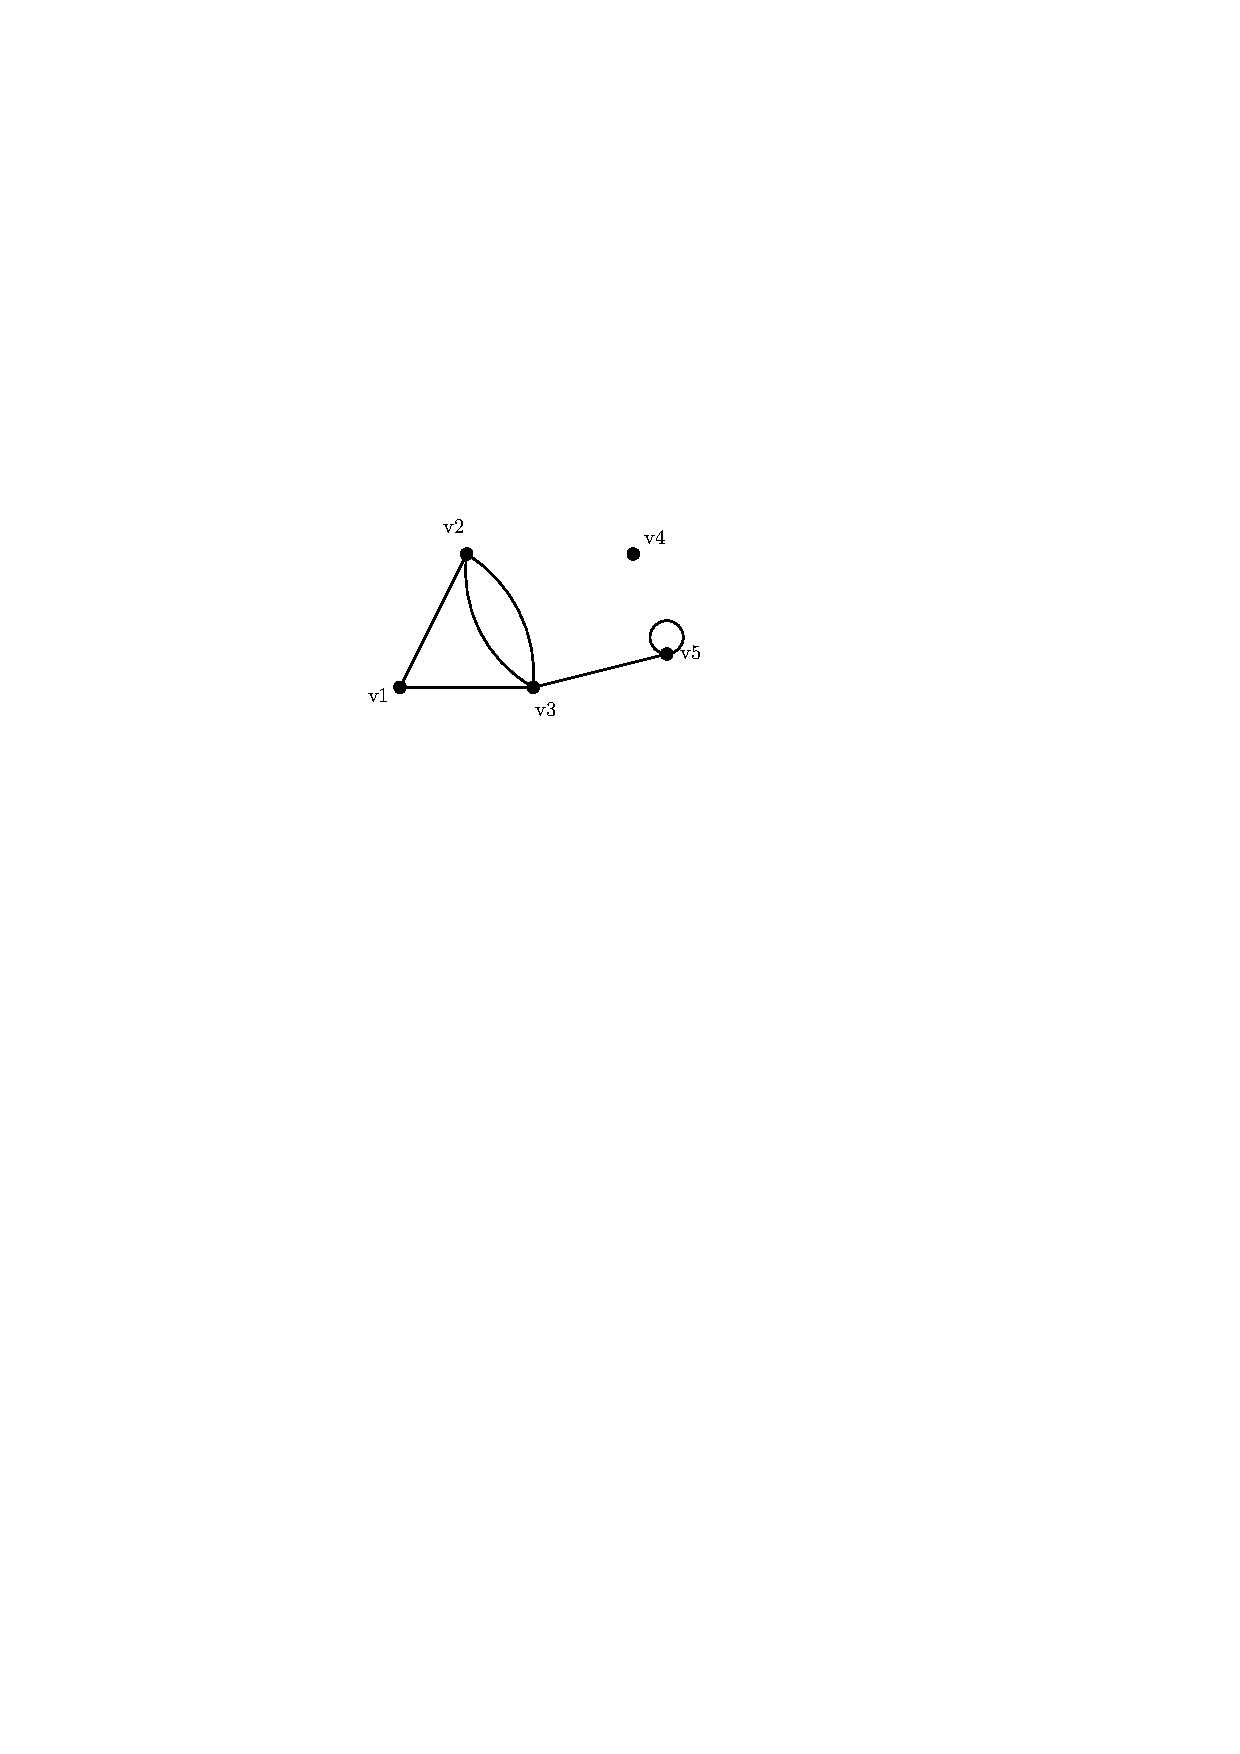
\includegraphics[width = \textwidth]{../media/simpel.pdf} \\
\caption{G}
\label{fig:simple}
\end{subfigure}
\begin{subfigure}{0.49\textwidth}
\centering
{
\begin{blockarray}{cccccc}
  & $v_{1}$ & $v_{2}$ & $v_{3}$ & $v_{4}$ & $v_{5}$ \\
\begin{block}{c(ccccc)}
  $v_{1}$ & 0 & 1 & 1 & 0 & 0 \\
  $v_{2}$ & 1 & 0 & 2 & 0 & 0 \\
  $v_{3}$ & 1 & 2 & 0 & 0 & 1 \\
  $v_{4}$ & 0 & 0 & 0 & 0 & 0 \\
  $v_{5}$ & 0 & 0 & 1 & 0 & 1 \\
\end{block}
\end{blockarray}
}
\vspace{0.1cm}
\caption{Adjazenzmatrix von G}
\label{mx:simple}
\end{subfigure}
\caption{Ein simpler Graph G}
\label{simpleGraph}
\end{figure}

Ein Vorteil von Graphen ist eine einfache Struktur.
Dabei werden die Ecken als Punkte und die Kanten als Linien oder Pfeile dargestellt (Abbildung ~\ref{fig:simple}) (\cite[49]{kurt}).
Zwischen zwei Ecken können einfache, mehrfache oder keine Kanten bestehen.
Darüber hinaus können sie mit sich selbst verbunden sein und eine sogenannte Schlinge bilden ($v_{5}$).
Sind zwei Ecken durch eine Kante verbunden werden sie als \textit{adjazent}(benachbart) bezeichnet.
Ist eine Ecke der Start- oder Endpunkt einer Kante, werden beide Objekte als \textit{inzident} zueinander bezeichnet.
Ist eine Ecke zu keiner Kante inzident heißt sie \textit{isoliert}.
Ein Graph der keine isolierten Ecken besitzt heißt \textit{zusammenhängend}.(\cite[4\psq]{theory}) \par

Computer können Graphen verarbeiten, da sich alle Ecken und Kanten in Form von Matrizen speichern lassen.
Die Abbildung ~\ref{mx:simple} zeigt die Adjazenzmatrix des Graphen aus ~\ref{fig:simple}.
Darin sind die Nachbarschaften für die jeweilige Eckenkombination gespeichert.
Die Reihen sind die Start- und die Spalten die Endecken.
Für eine existierende Kante wird eine ~$1$ und für keine Verbindung eine ~$0$ eingetragen.
Die ~$2$ in Spalte $v_{2}$ und Reihe $v_{3}$ zeigt die Mehrfachkante zwischen den beiden Ecken an.
Für ungerichtete Graphen ist eine Kante von $v_{1}$ nach $v_{2}$ äquivalent mit einer Kante von $v_{2}$ nach $v_{1}$.
Daher ist die Adjazenzmatrix für ungerichtete Graphen spiegelsymmetrisch entlang der Hauptdiagonale ($v_{1}v_{1} \rightarrow v_{5}v_{5}$).
Der Speicherbedarf für eine Matrix wird folglich halbiert, da die eine Hälfte mit der Anderen rekonstruiert werden kann (Abb.~\ref{mx:iso}).
Besitzt der Graph keine Schlingen, besteht die Hauptdiagonale lediglich aus Nullen und kann ebenfalls eingespart werden (\cite[19]{algorithms}).

Im Folgenden werden nur zusammenhängende Graphen ohne Schlingen betrachtet, da diese für viele Problemstellungen irrelevant sind (\cite[4\psq]{theory}).

\begin{figure}[htb]
\centering
\begin{subfigure}{0.42\textwidth}
\centering
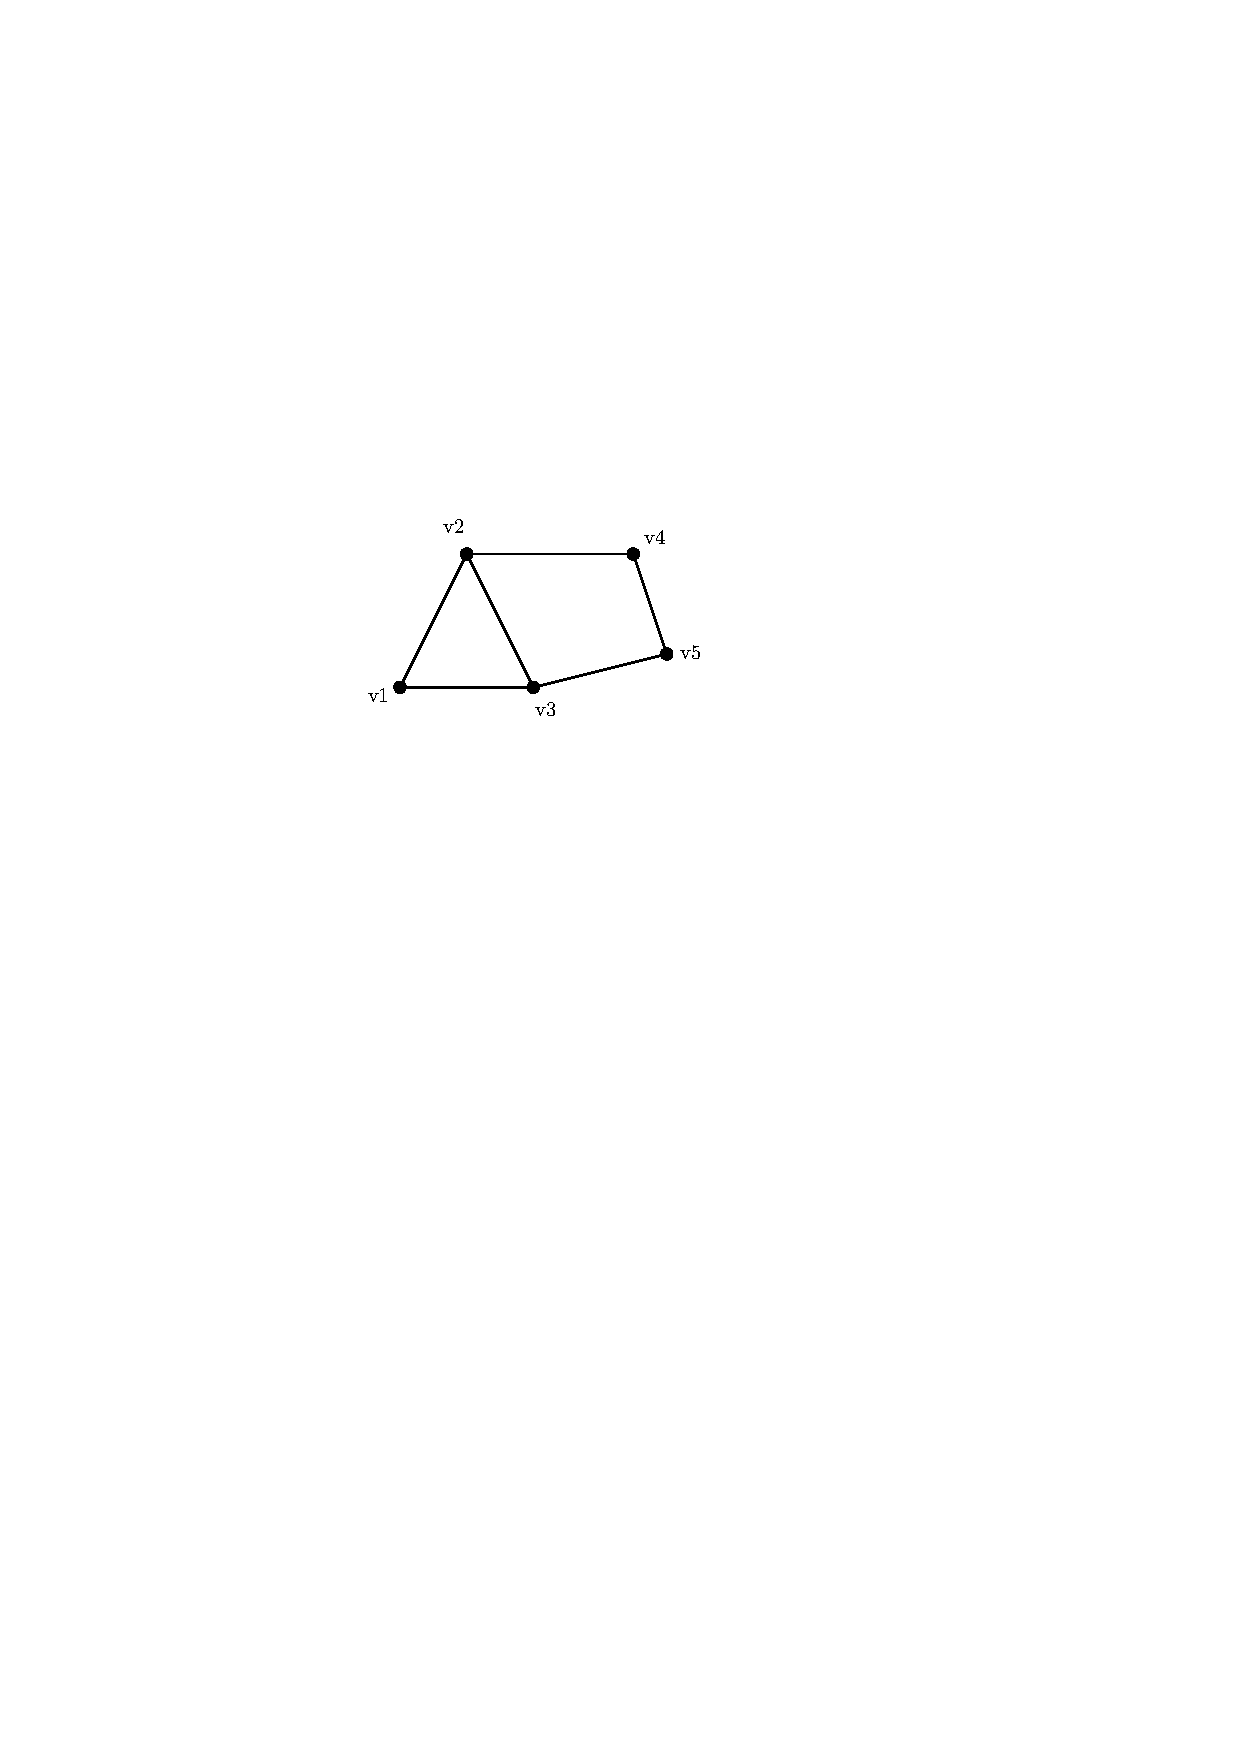
\includegraphics[width = \textwidth]{../media/iso1.pdf} \\
\caption{G}
\label{fig:iso1}
\end{subfigure}
\hspace{2cm}
\begin{subfigure}{0.30\textwidth}
\centering
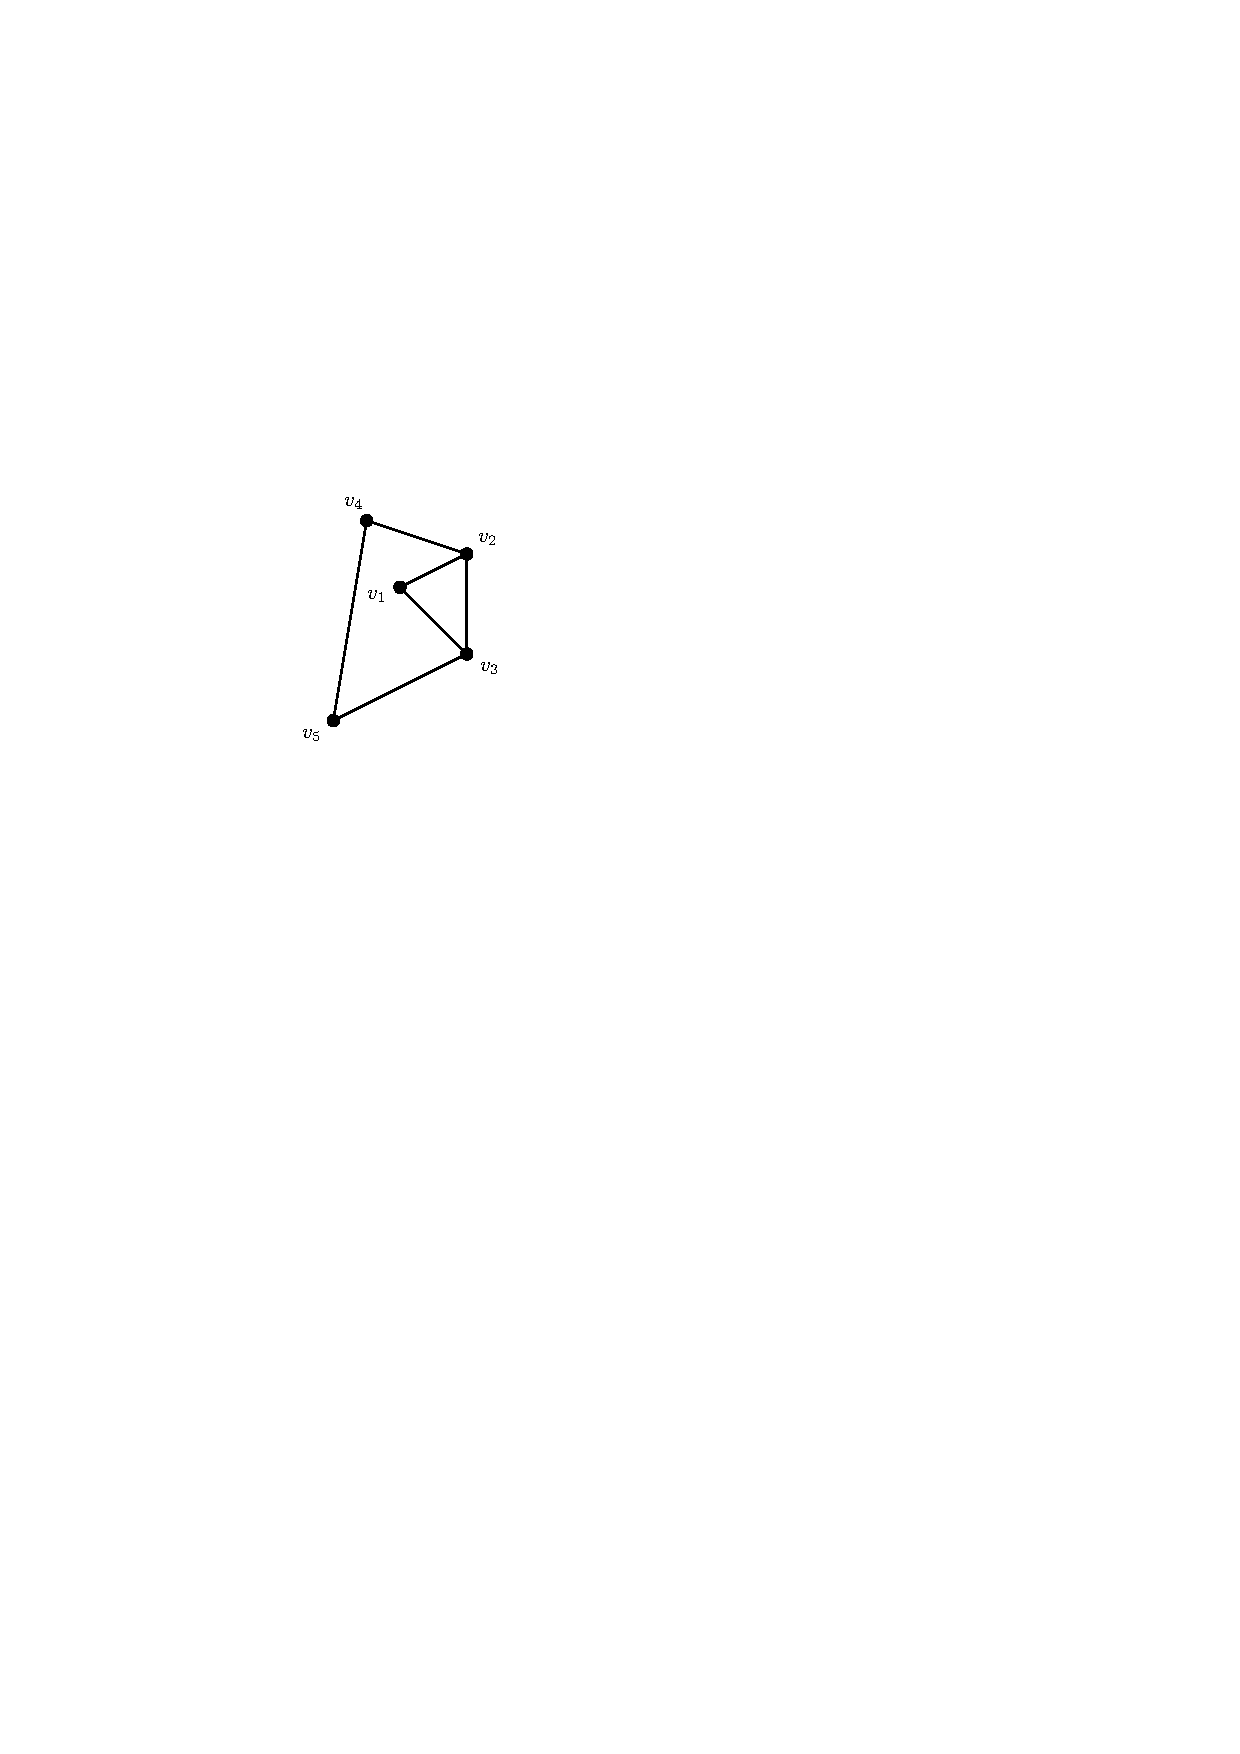
\includegraphics[width = \textwidth]{../media/iso2.pdf} \\
\caption{H}
\label{fig:iso2}
\end{subfigure}
\begin{subfigure}{0.40\textwidth}
\centering
\vspace{0.5cm}
{
\begin{blockarray}{cccccc}
  & $v_{1}$ & $v_{2}$ & $v_{3}$ & $v_{4}$ & $v_{5}$ \\
\begin{block}{c(ccccc)}
  $v_{1}$ & $\ddots$ & 1 & 1 & 0 & 0 \\
  $v_{2}$ &   & $\ddots$ & 1 & 1 & 0 \\
  $v_{3}$ &   &   & $\ddots$ & 0 & 1 \\
  $v_{4}$ &   &   &   & $\ddots$ & 1 \\
  $v_{5}$ &   &   &   &   & $\ddots$ \\
\end{block}
\end{blockarray}
}
\caption{Adjazenzmatrix von G und H}
\label{mx:iso}
\end{subfigure}
\caption{Zwei isomorphe Graphen G und H}
\label{isoGraph}
\end{figure}

Wenn zwei Graphen bei gleichbleibenden Nachbarschaften der Ecken aufeinander abgebildet werden können, spricht man von isomorphen Graphen (\cite[106]{theory}).
Daraus ergibt sich für isomorphe Graphen auch immer eine gleiche Adjazenzmatrix (Abb.~\ref{isoGraph}).


\subsubsection{Gerichtete Graphen}
Im Gegensatz zu einem ungerichteten Graphen können bei einem gerichteten Graphen Kanten lediglich in einer Richtung durchlaufen werden.
Die Kanten werden daher durch Pfeile anstatt Linien dargestellt.

$$G = (V,R)$$

Demnach muss in Abbildung~\ref{fig:directed} um von $v_{5}$ nach $v_{4}$ zu gelangen der Weg über die Ecken $v_{3}$ und $v_{2}$ führen.

\begin{figure}[htb]
\centering
\begin{subfigure}{0.49\textwidth}
\centering
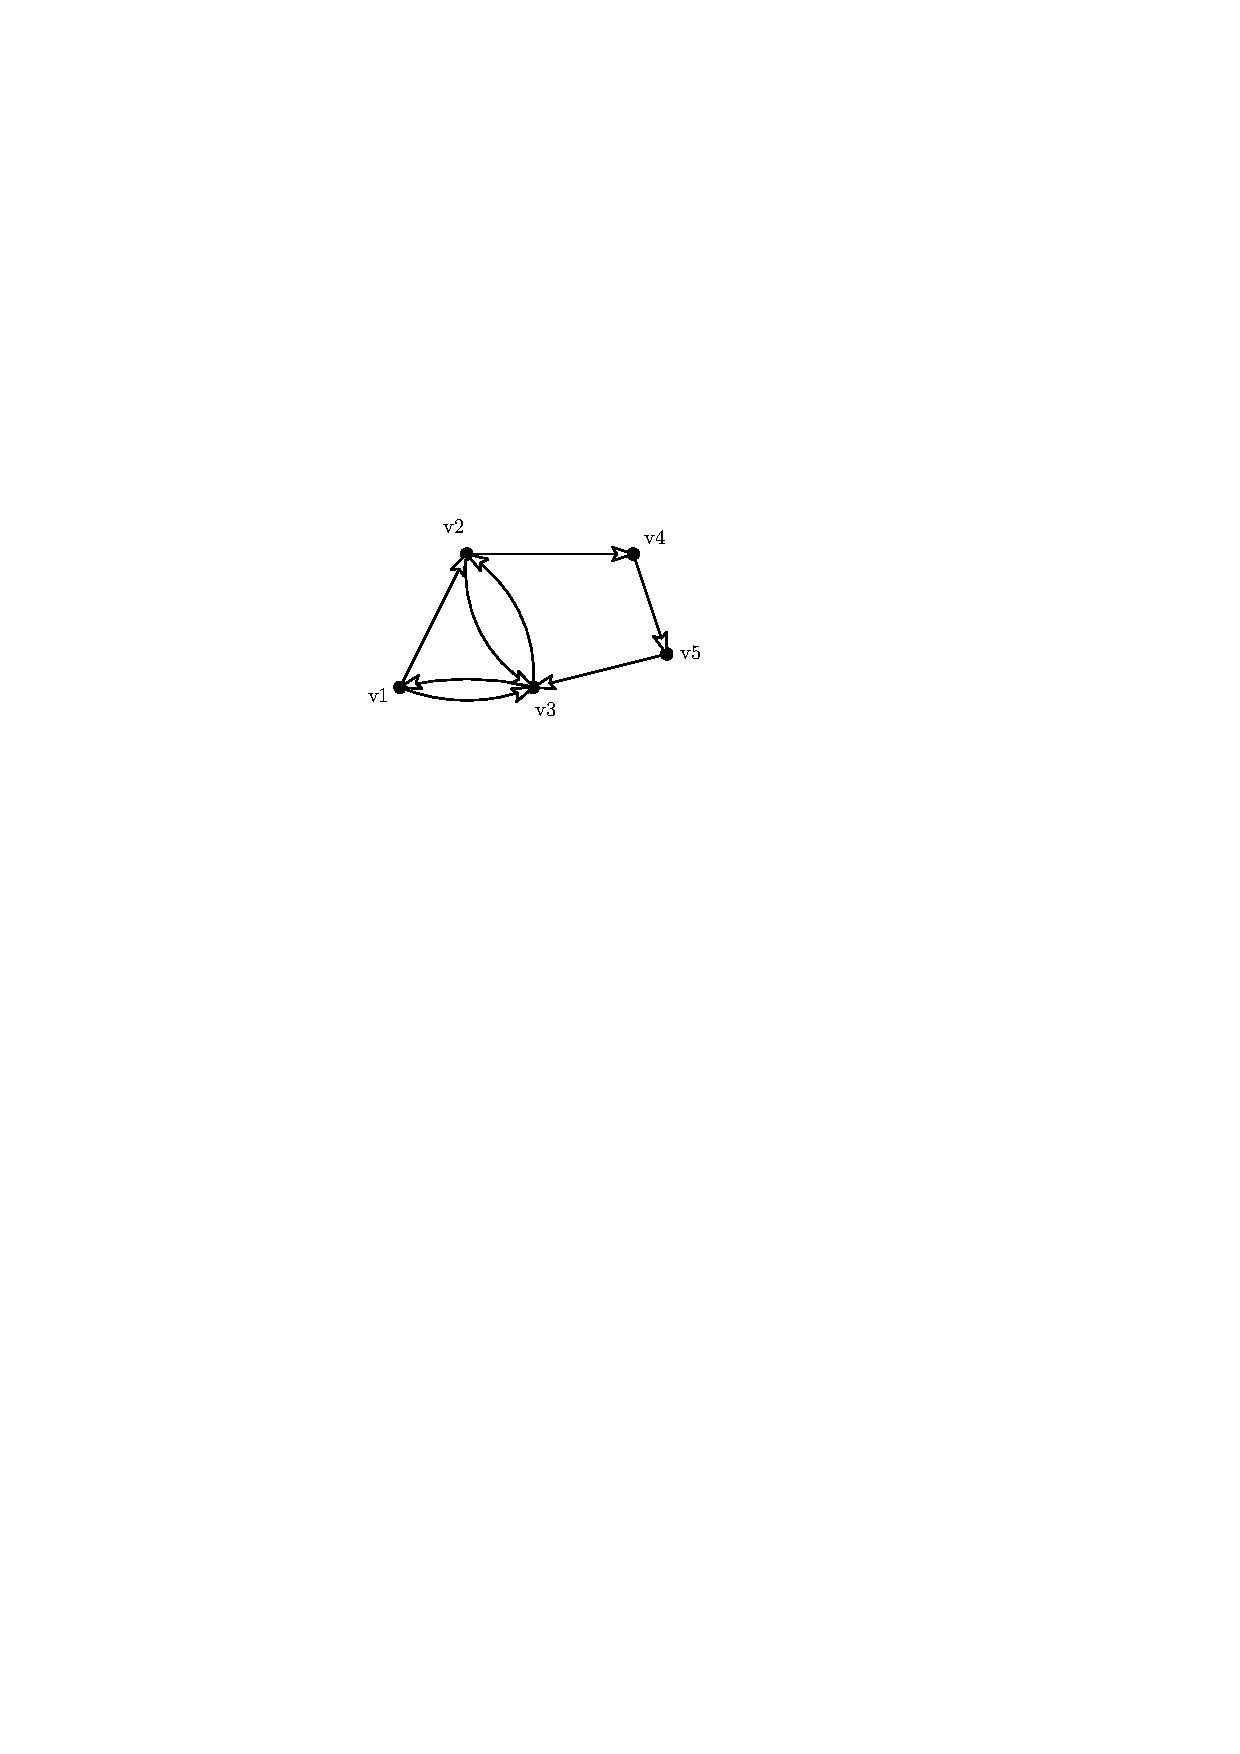
\includegraphics[width = \textwidth]{../media/gerichtet.pdf} \\
\caption{G}
\label{fig:directed}
\end{subfigure}
\begin{subfigure}{0.49\textwidth}
\centering
{
\begin{blockarray}{cccccc}
  & $v_{1}$ & $v_{2}$ & $v_{3}$ & $v_{4}$ & $v_{5}$ \\
\begin{block}{c(ccccc)}
  $v_{1}$ & 0 & 1 & 1 & 0 & 0 \\
  $v_{2}$ & 0 & 0 & 1 & 1 & 0 \\
  $v_{3}$ & 1 & 1 & 0 & 0 & 0 \\
  $v_{4}$ & 0 & 0 & 0 & 0 & 1 \\
  $v_{5}$ & 0 & 0 & 1 & 0 & 0 \\
\end{block}
\end{blockarray}
}
\vspace{0.1cm}
\caption{Adjazenzmatrix von G}
\label{mx:directed}
\end{subfigure}
\caption{Ein gerichteter Graph G}
\label{directedGraph}
\end{figure}

\subsubsection{Gewichtete Graphen}
In dieser Arbeit bezeichnet der Begriff \textit{gewichteter Graph} einen Kanten-gewichteten Graphen, bei dem jeder Kante ein Wert ~$c$ zugewiesen wird.

$$G = (V,E)$$ 
\begin{center}
mit
\end{center}
$$c: E \rightarrow \mathbb{R}$$

Neben dem Kanten-gewichteten gibt es auch Ecken-gewichtete Graphen, bei welchen entsprechend die Ecken gewichtet werden.
Diese werden aber nur für wenige Problemstellungen benötigt und sind hier nicht von Belang.
Gewichtete Graphen können gerichtet und ungerichtet sein.
Ein klassisches Beispiel hierfür ist der Linien-Netzplan einer Straßenbahn, bei dem die Ecken einzelne Haltestellen darstellen und die Kantengewichte die benötigten Minuten beinhalten.

\begin{figure}[htb]
\centering
\begin{subfigure}{0.49\textwidth}
\centering
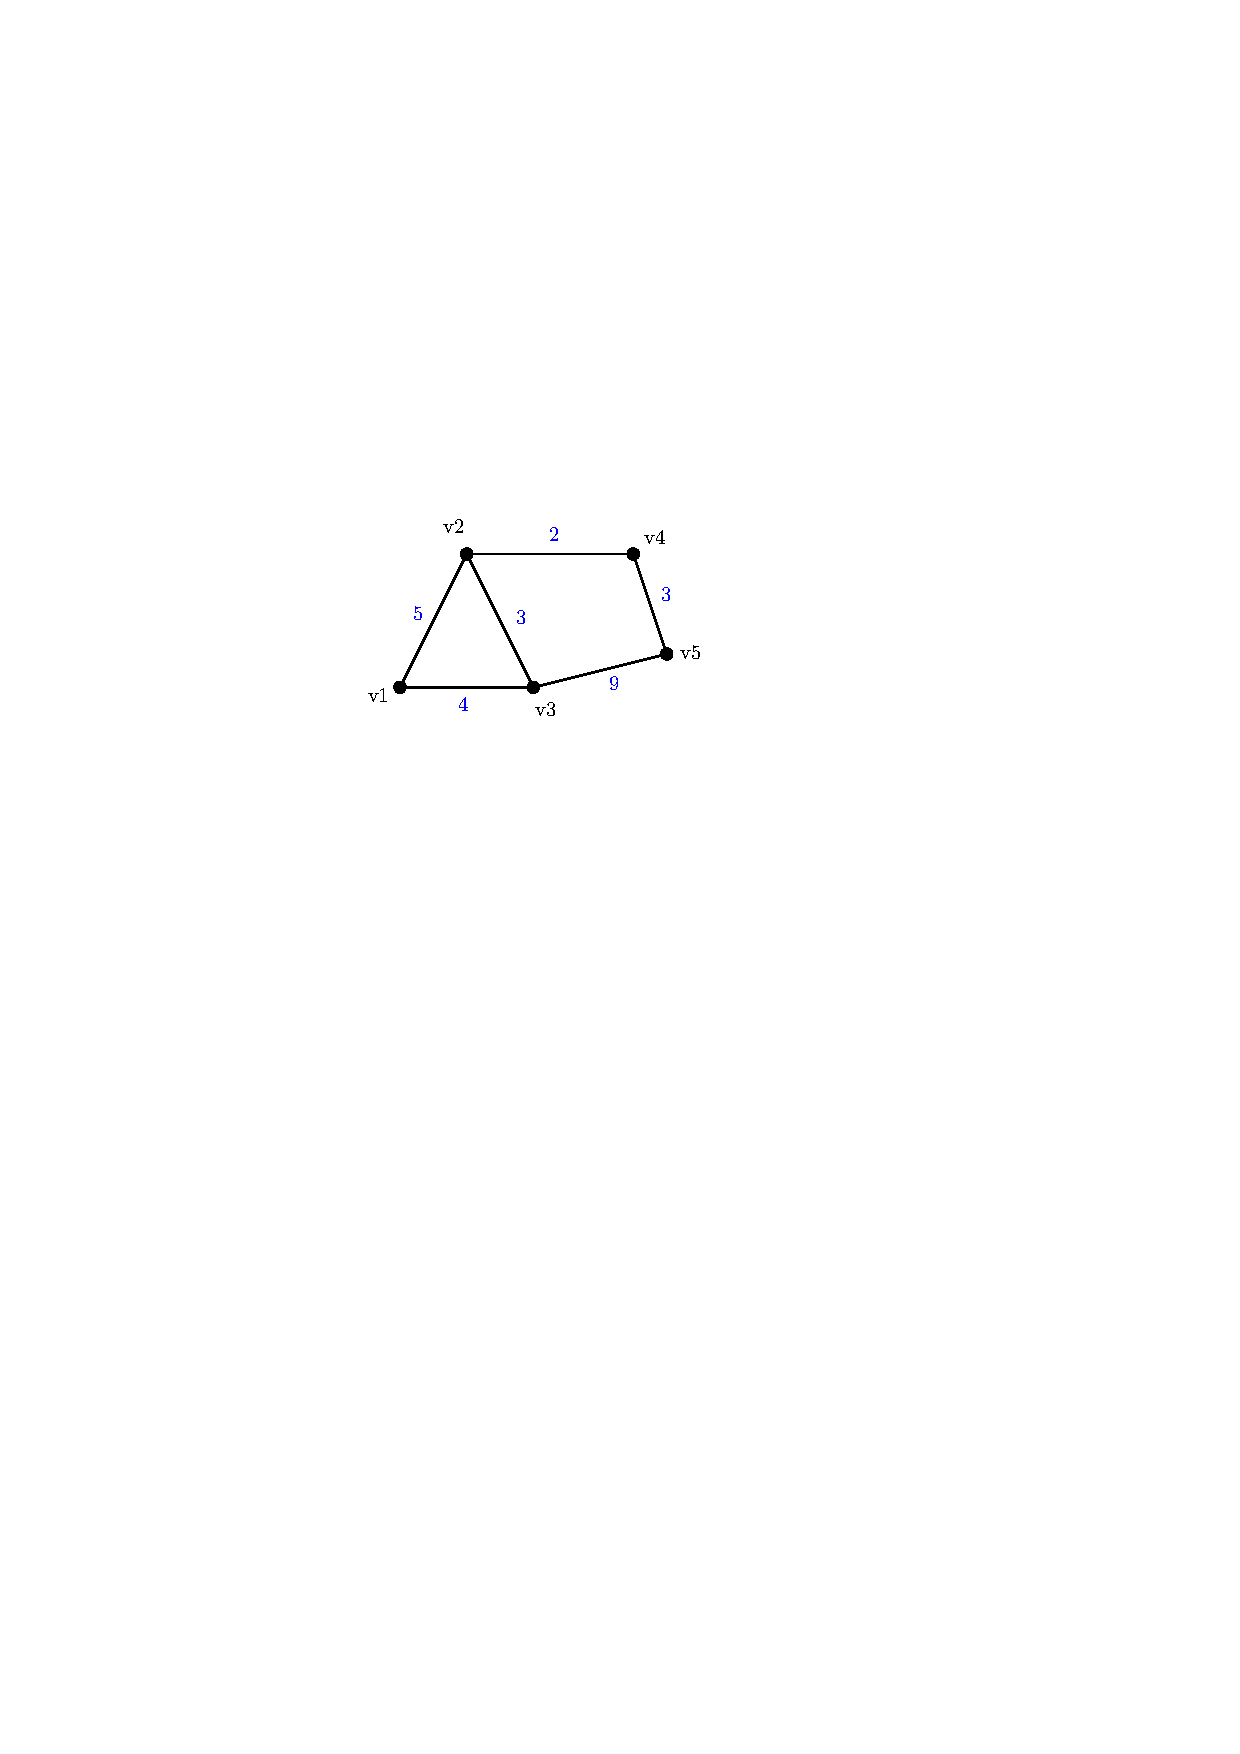
\includegraphics[width = \textwidth]{../media/gewichtet.pdf} \\
\caption{G}
\label{fig:weighted}
\end{subfigure}
\begin{subfigure}{0.49\textwidth}
\centering
{
\begin{blockarray}{cccccc}
  & $v_{1}$ & $v_{2}$ & $v_{3}$ & $v_{4}$ & $v_{5}$ \\
\begin{block}{c(ccccc)}
  $v_{1}$ & 0 & 5 & 4 & 0 & 0 \\
  $v_{2}$ & 5 & 0 & 3 & 2 & 0 \\
  $v_{3}$ & 4 & 3 & 0 & 0 & 9 \\
  $v_{4}$ & 0 & 2 & 0 & 0 & 3 \\
  $v_{5}$ & 0 & 0 & 9 & 3 & 0 \\
\end{block}
\end{blockarray}
}
\vspace{0.1cm}
\caption{Adjazenzmatrix von G}
\label{mx:weighted}
\end{subfigure}
\caption{Ein gewichteter Graph G}
\label{weightedGraph}
\end{figure}

Mit gewichteten Graphen können diverse Problemstellungen gelöst werden, zum Beispiel die Bestimmung maximaler (Durch-)Flüsse in Rohrsystemen oder das Berechnen kürzester Wege.
Andererseits kann ein gewichteter Graph auch für Routing-Zwecke eingesetzt werden, indem räumliche Positionen sowie Eigenschaften von Straßen in der Datenstruktur eines Graphen gespeichert werden.

\subsubsection{Erstellung eines Graphen aus OpenStreetMap-Daten}
\label{sec:osmgraph}

Die \gls{osm}\footnote{OpenStreetMap ist ein 2004 gegründetes internationales Projekt mit dem Ziel, eine freie Weltkarte zu erschaffen (\href{www.openstreetmap.de}). Die Daten werden von vielen Freiwilligen auf der ganzen Welt generiert und in einer Datenbank unter der Open Database Lizenz zur verfügung gestellt.} Datenstruktur kann als Graph abgebildet werden.
Hier werden Punktobjekte als \textit{Nodes} (Knoten) und Linienobjekte wie Straßen als \textit{Ways} (Wege) bezeichnet.
Ein Way ist dabei die Verbindung zwischen zwei oder mehreren Nodes.
Zusätzlich gibt es \textit{Relations} (Relationen) die eine Menge aus Nodes und Ways einen funktionalen Zusammenhang zuschreiben.
Für Straßennetze kann dies durchaus hilfreich sein um beispielsweise unterschiedliche Segmente eines Autobahnsegmentes zusammenzufassen oder um Abbiegevorschriften an Kreuzungen zu beschreiben (\cite{osmrelation}).

Um aus den \gls{osm} Daten einen routingfähigen Graphen zu erhalten, müssen zuerst alle benutzbaren Nodes und Ways extrahiert werden um sie dann anhand ihrer \gls{osm}-Tags zu identifizieren.
Dazu gehören alle Arten von Straßen und Wegen sowie als befahrbar gekennzeichnete Ways (beispielsweise asphaltiert, allerdings ohne angegebenen Straßentyp).
Für das Routing sind vor allem Verbindungspunkte wie Kreuzungen, Ab- und Auffahrten sowie Sackgassen wichtig.
Daher werden diese sogenannten \textit{Tower Nodes} aus den importierten Daten ermittelt.
Anschließend werden die Straßen anhand der Verbindungspunkte segmentiert.
Danach werden die Verbindungen zwischen den Tower Nodes berechnet und anhand der Distanz gewichtet.
Das Grundgerüst des eigentlichen Routing-Graphen ist damit erstellt.
Einbahnstraßen und Abbiegebeschränkungen werden berücksichtigt und geben die Richtung der Kanten an (\cite{osmgraph}).
Die Punkte zwischen zwei Tower Nodes werden \textit{Pillar Nodes} genannt.
Sie werden als \textit{WayGeometry} auf der jeweiligen Kante gespeichert, da sie nicht für den Routing Vorgang benötigt werden (Abbildung ~\ref{fig:tower}).
Das Routing ist dadurch um ungefähr das 8-fache schneller (\cite{graphhopper}).
Relevante Attribute wie Geschwindigkeit oder Straßentyp werden vereinheitlicht und als \textit{Flags} (Markierungen) auf der Kante gespeichert.
Diese sind für die individuelle Gewichtung bei der Routenfindung interessant.
(Mehr zu Gewichtung später in Kapitel ~\ref{backendGraphBuild}).
Zuletzt wird der Graph abgespeichert und ist für Routing Abfragen bereit (\cite{osmgraph}).

\begin{figure}[htb]
\centering
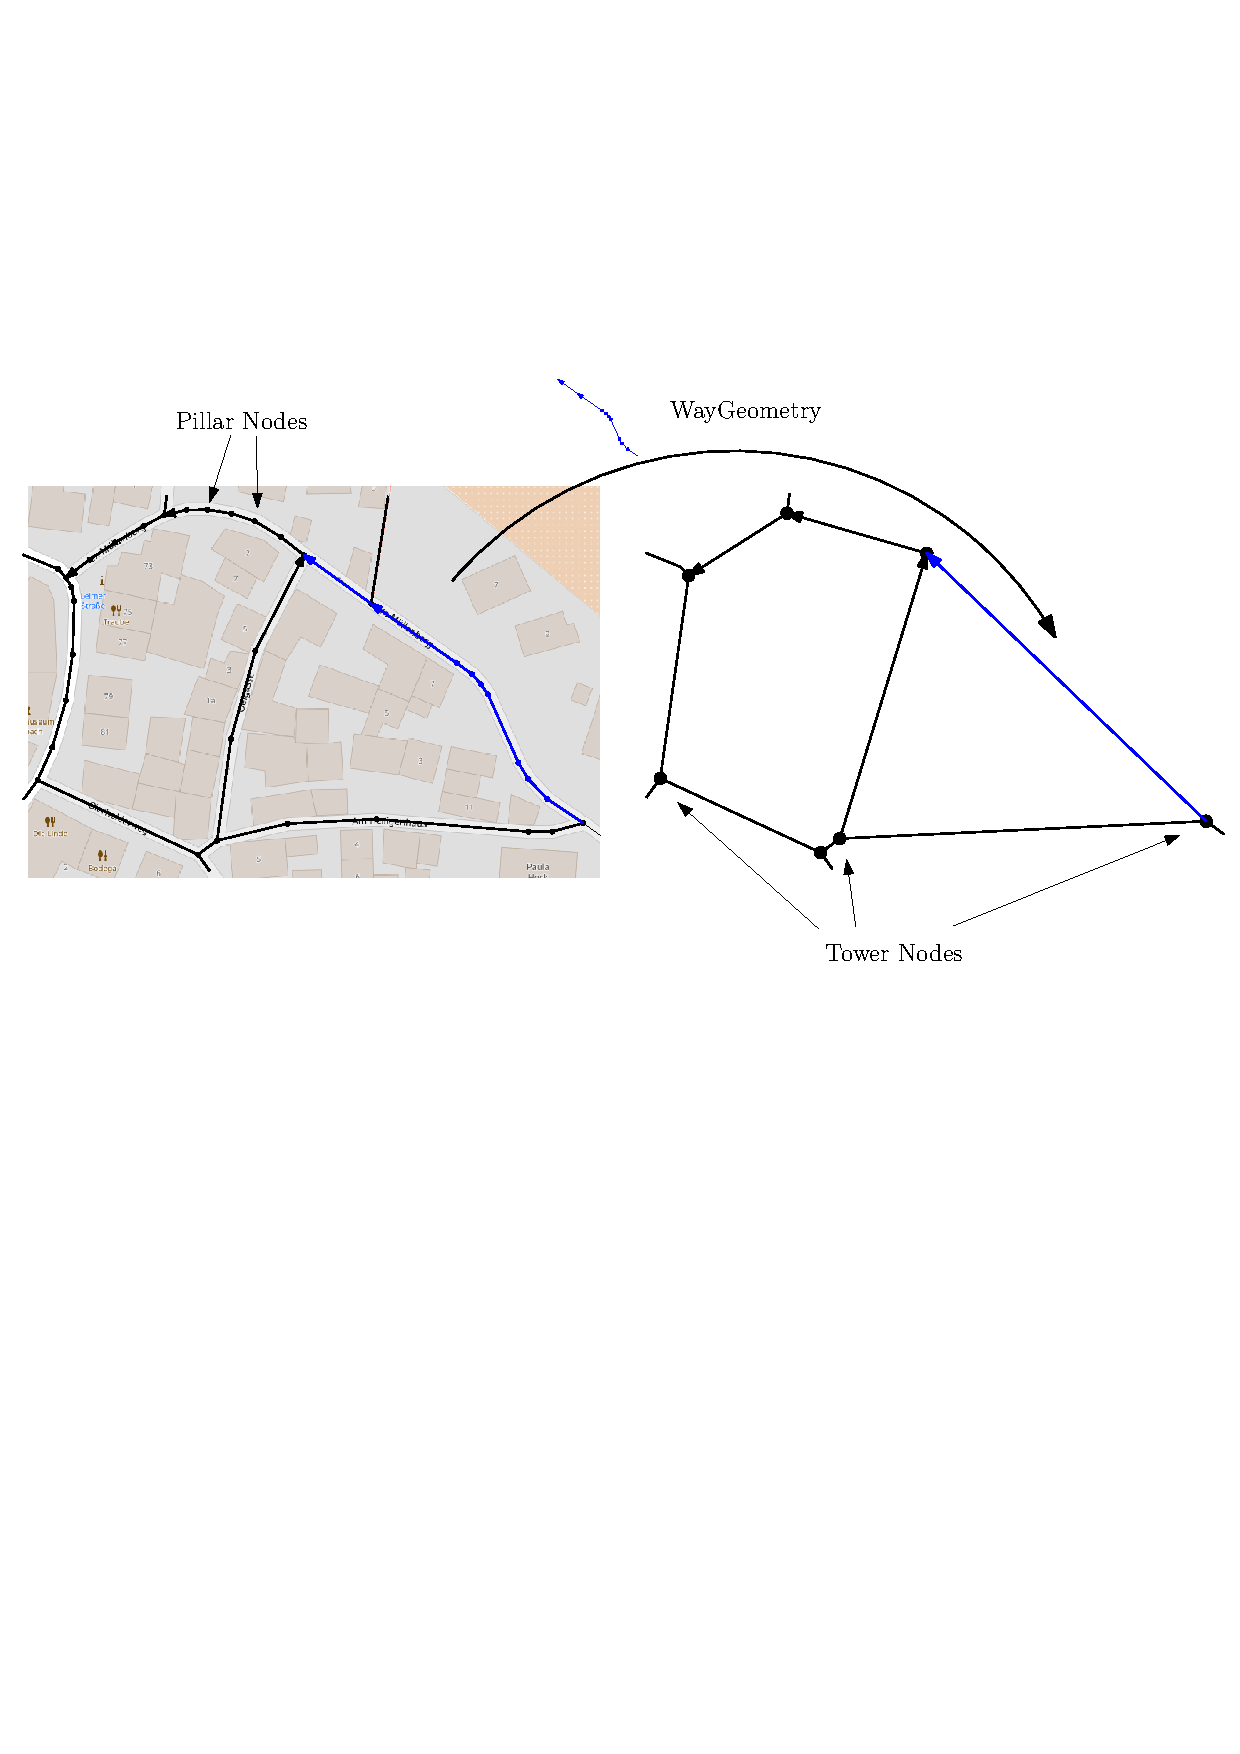
\includegraphics[width = \textwidth]{../media/towers.pdf} \\
\caption{Simplifizierung eines \gls{osm} Datensatzes}
\label{fig:tower}
\end{figure}

\subsection{Routing}

Routing bezeichnet den Vorgang in einem Netzwerk Wege zu finden, auf denen Datenpakete entlang gesendet werden können.
Diese Definition bezieht sich vor allem auf elektronische Datennetzwerke wie das Telefonnetz oder das Internet.
Im Fachbereich der Geoinformationssysteme werden hauptsächlich Straßennetze für Routing-Analysen verwendet (\cite[165]{handbook}).
Ein Weg \textit{P} (\textit{engl: path}) von einer Startecke ~$s$ zu einemr Zielecke ~$z$ ist eine Folge von benachbarten Ecken mit $s~$ als erste Ecke und $z~$ als letzte Ecke der Folge.
Die Weglänge entspricht in einem gewichteten Graphen der Summe aller Kantengewichte.

Eine der wichtigsten Netzwerk-Analyse-Operationen ist die Berechnung des kürzesten Weges zwischen zwei Ecken.
Jedes Navigationssystem muss diese Aufgabe erfüllen können.
Ein kürzester Weg hat demnach die Eigenschaft, dass die Summe aller Kantengewichte, in anderen Worten die Kosten des Weges, minimal gegenüber allen anderen Wegen im Graphen ist.

\subsubsection{Shortest Path Problem}
Die nächstliegendste zu beleuchtende Problemstellung ist das \textit{Shortest Path Problem} welches aber nicht mit dem \textit{\gls{tsp}} verwechselt werden sollte.
Beim \gls{tsp} ist die kürzeste Tour auf einem Graphen $G = (V,E) = K_{n}$\footnote{$K_{n}$ bezeichnet einen vollständigen Graphen bei dem jede Ecke aus V mit jeder anderen Ecke verbunden ist} mit der Gewichtsfunktion $c: E \rightarrow \mathbb{R}_{+}$ gesucht, die jede Ecke des Graphen besucht (\cite[135]{algorithms}).
Das Shortest Path Problem lässt sich in drei Typen untergliedern denen jeweils ein gerichteter Graph $G = (V,E)$ mit der Gewichtsfunktion $c: E \rightarrow \mathbb{R}$ zugrunde liegt.
Beim \textit{\gls{spp}} wird der kürzeste Weg von einer Ecke $a~$ zu einer anderen Ecke $b~$ mit $a,b\in V$ gesucht.
Das \textit{\gls{ssp}} möchte den kürzesten Weg einer Ecke $a~$ zu jeder anderen Ecke ermitteln (Formel ?).
Das \textit{\gls{apsp}} sucht den kürzesten Weg von jeder Ecke zu jeder anderen Ecke in $V~$ (\cite[169\psq]{algorithms}).

Für eine Route von Startecke $s~$ zur Zielecke $z~$ ist das \gls{spp} demnach die richtige Wahl.
Allerdings wird dazu das \gls{ssp} herangezogen, welches mit dem Algorithmus von Dijkstra gelöst werden kann.


\subsubsection{Dijkstra-Algorithmus}
\label{sec:dijkstra}
Der in 1959 von Edsger W. Dijkstra entwickelte Algorithmus (\cite{dijkstra}) benötigt einen gewichteten Graphen ohne negative Kantengewichte\footnote{Das Problem bei Graphen mit negativer Gewichtung entsteht, wenn diese auf einer Schlinge oder der Kante eines Rings liegen.
Sobald der Algorithmus den Zyklus erreicht, werden die Kosten für die Ecken des Zyklus immer geringer.
Die Kosten für den kürzesten Weg nähern sich $-\infty $ während der Algorithmus in einer endlos Schleife läuft.
Deswegen ist der Dijkstra nur für positive Kantengewichte anwendbar (\cite[194\psq]{kurt})} sowie eine Startecke $s \in V$.
Es gibt eine Warteliste $W_{s}$ mit unmarkierten \textit{gesichteten} Ecken.
Dort sind für alle $v~$ die Kosten für den bisher kürzesten Weg von $s~$ und die jeweilige vorangehende Ecke auf diesem Weg gespeichert.
Die Kosten können sich noch ändern wenn ein noch kürzerer Weg gefunden wird.
Diese Liste enthält zu Beginn nur den Startpunkt $s~$ mit den trivialen Kosten $0~$.
Es gibt eine weitere Liste der endgültig kürzesten Wege $K_{s}$ in der alle markierten Ecken gespeichert werden.

Dijkstra's Algorithmus markiert die Ecke mit den geringsten Kosten aus $W_{s}$ und verschiebt diese nach $K_{s}$.
Nun werden alle benachbarten Ecken gesichtet und die Kosten berechnet.
Die Kosten und der Vorgänger werden in $W_{s}$ gespeichert.
Die Ecke mit den geringsten Kosten wird als nächstes markiert, da der Weg dorthin auf jeden Fall ein kürzester ist.
Dieser Vorgang wird wiederholt bis alle Ecken aus $W_{s}$ markiert wurden und $W_{s}$ somit leer ist.

% Init Dijkstra
\begin{figure}[htb]
\centering
\begin{subfigure}{0.49\textwidth}
\centering

\includegraphics[width = \textwidth]{../media/dijkstra.pdf} \\
\caption{G}
\label{fig:dijkstra}
\end{subfigure}
\begin{subfigure}{0.49\textwidth}
\centering
{
\begin{blockarray}{cccccc}
  & $v_{1}$ & $v_{2}$ & $v_{3}$ & $v_{4}$ & $v_{5}$ \\
\begin{block}{c(ccccc)}
  $v_{1}$ & 0 & 5 & 4 & 0 & 0 \\
  $v_{2}$ & 7 & 0 & 0 & 3 & 0 \\
  $v_{3}$ & 4 & 2 & 0 & 0 & 8 \\
  $v_{4}$ & 0 & 3 & 6 & 0 & 1 \\
  $v_{5}$ & 0 & 0 & 8 & 1 & 0 \\
\end{block}
\end{blockarray}
}
\vspace{0.1cm}
\caption{Adjazenzmatrix von G}
\label{mx:dijkstra}
\end{subfigure}
\caption{Ein gewichteter und gerichteter Graph G}
\label{dijkstraGraph}
\end{figure}

Die Funktionsweise des Dijkstra Algorithmus wird am Graphen aus Abbildung~\ref{dijkstraGraph} mit der Startecke $s=v_{1}$ veranschaulicht.

Die erste Ecke der Warteschlange ist $s=v_{1}$.
Da $s~$ der einzige Eintrag ist, sind die Kosten automatisch am geringsten.
$s~$ wird von $W_{s}$ nach $K_{s}$ verschoben, markiert und die erreichbaren Ecken gesichtet.
Das sind $v_{2}$ mit den Kosten $5~$ und $v_{3}$ mit den Kosten $4~$.
Beide werden mit $v_{1}$ als Vorgänger in $W_{s}$ eingetragen.
Im zweiten Durchgang wird $v_{3}$ (geringste Kosten in $W_{s}$) markiert und nach $K_{s}$ verschoben.
Über $v_{3}$ erreichbare Ecken sind $v_{5}$ mit $4+8=12$ Kosten und $v_{2}$ mit $4+2=6$ Kosten.
Da bereits ein kürzerer Weg nach $v_{2}$ besteht wird der aktuelle Pfad über $v_{3}$ verworfen.
Als nächstes wird $v_{2}$ nach $K_{s}$ verschoben.
Die einzige neue von dort gesichtete Ecke ist $v_{4}$ mit $8~$ Kosten.
Bei der vierten Wiederholung wird $v_{4}$ ($8<12$) markiert.
Es werden $v_{3}$ und $v_{5}$ gesichtet.
Für $v_{3}$ besteht bereits ein kürzerer Weg.
Für $v_{5}$ ist der neue Weg über $v_{4}$ mit den Kosten von $9~$ allerdings kürzer als der Weg über $v_{3}$.
$v_{5}$ wird aktualisiert und der längere Pfad verworfen.
Im fünften Durchgang wird $v_{5}$ als letzte Ecke in $W_{s}$ nach $K_{s}$ verschoben.
Von dort sind keine neuen Ecken sichtbar.
Die Warteschlange ist leer und der Algorithmus damit beendet.

\begin{figure}[htb]
\centering
\begin{subfigure}{0.32\textwidth}
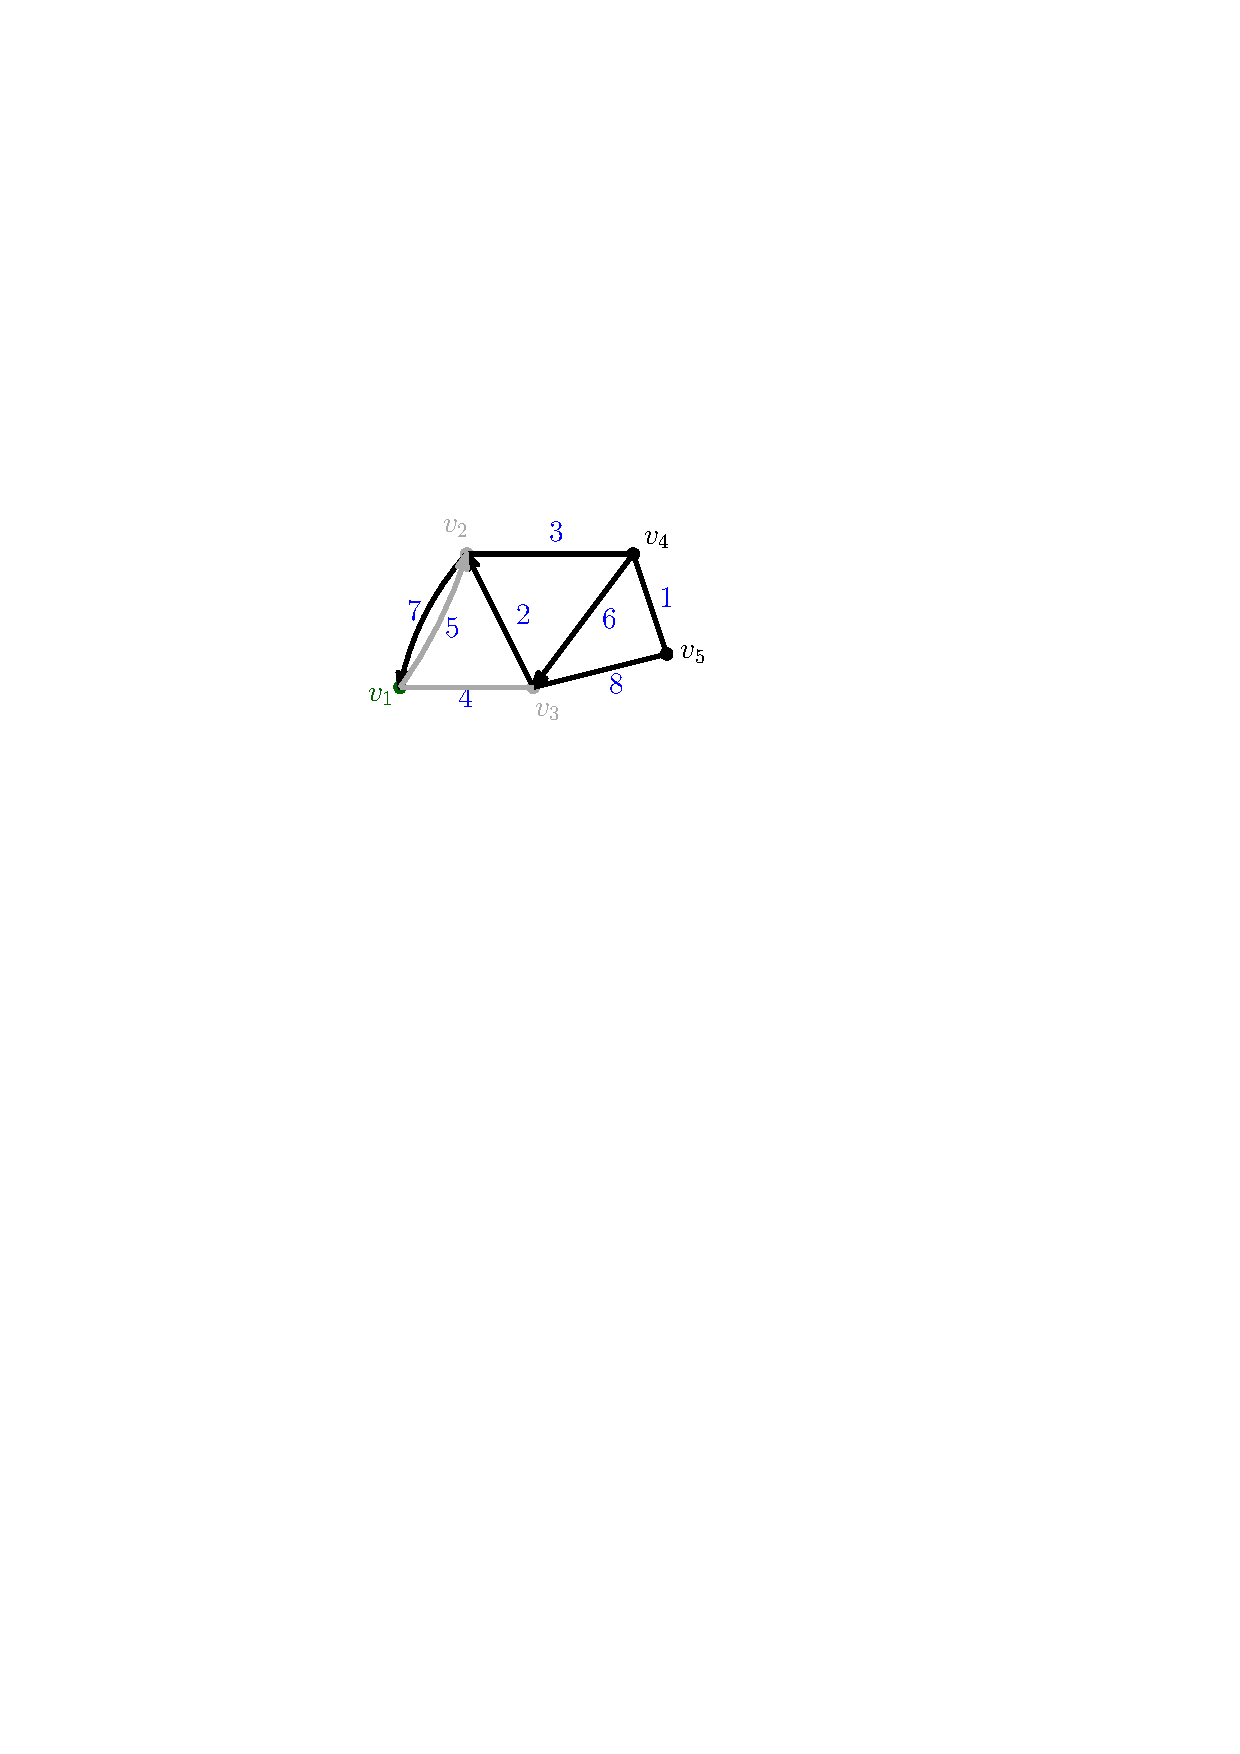
\includegraphics[width = \textwidth]{../media/dijkstra1.pdf} \\
\caption{1. Iteration}
\vspace{0.5cm}
\label{fig:dijkstra1}
\end{subfigure}
\begin{subfigure}{0.32\textwidth}
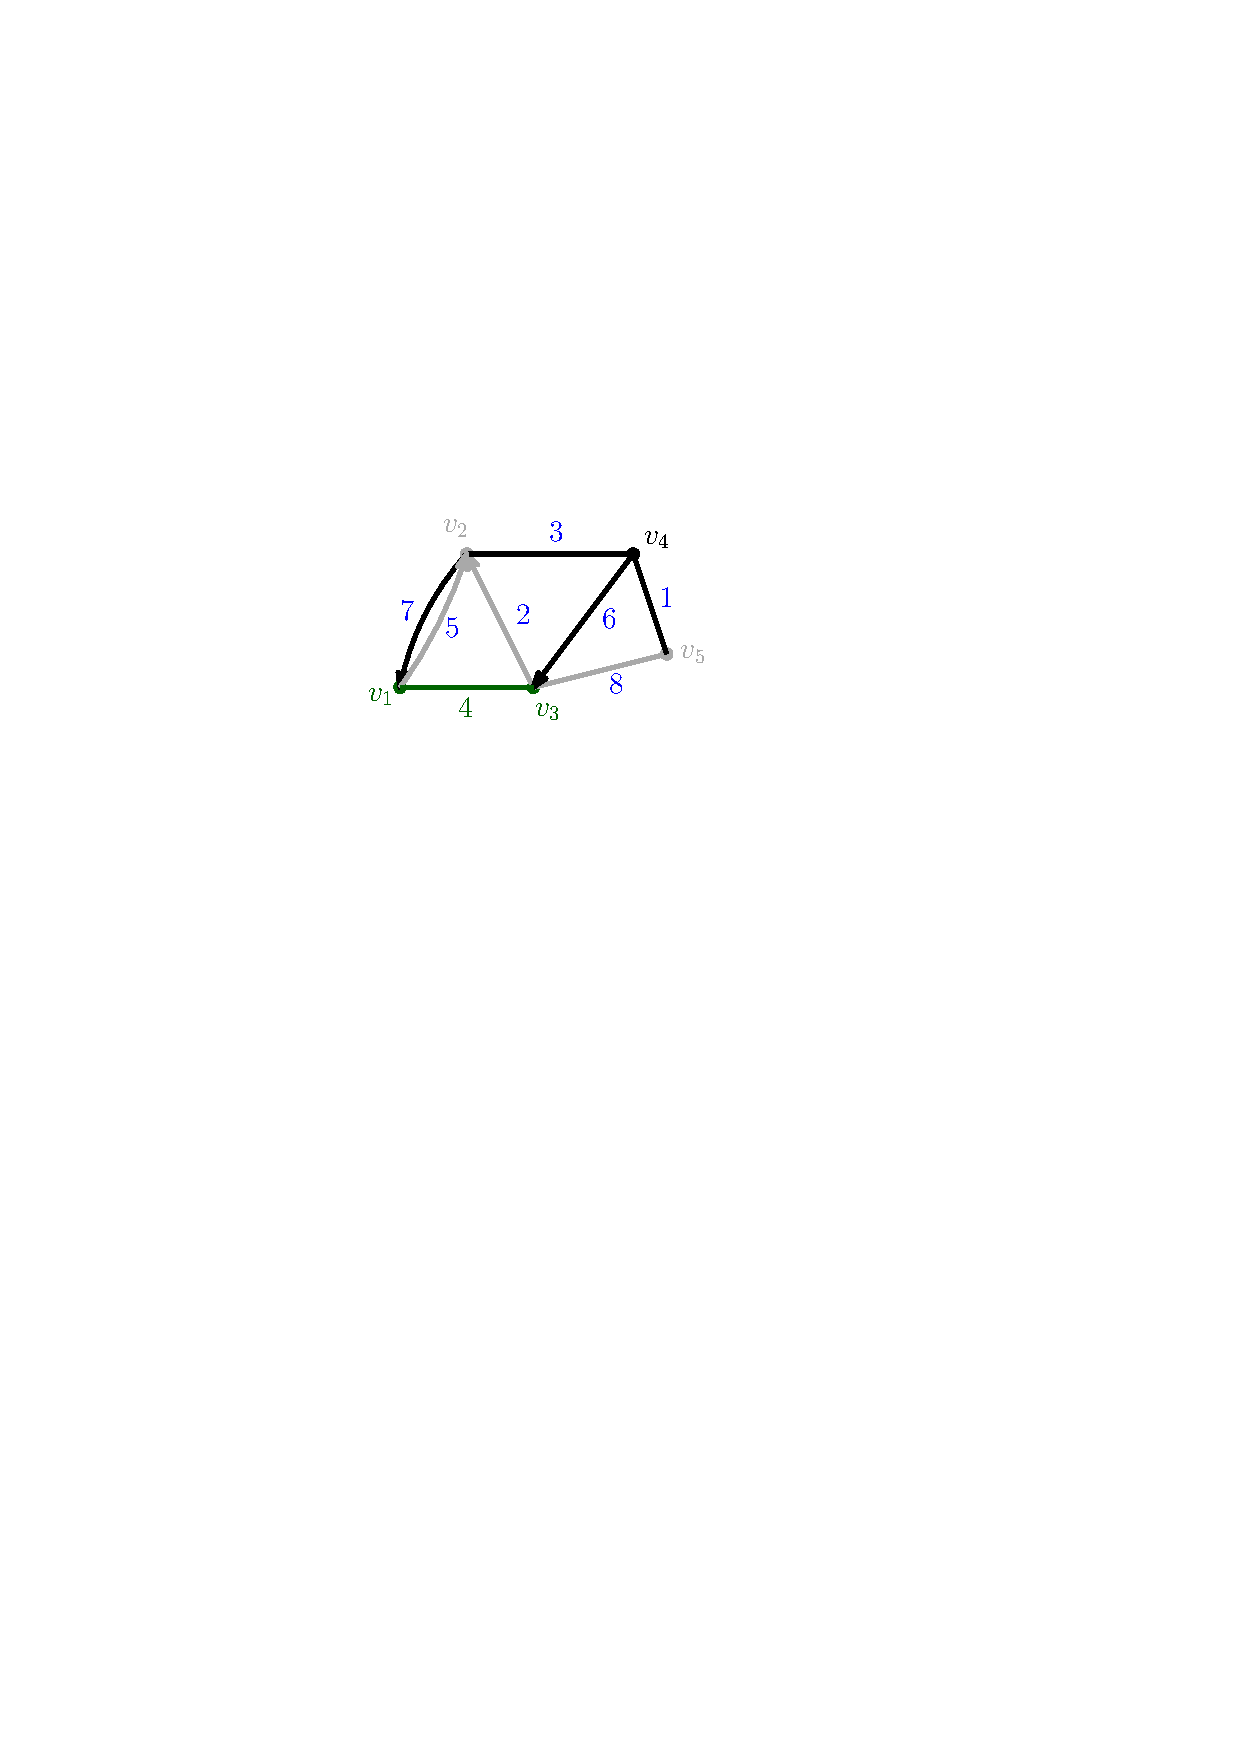
\includegraphics[width = \textwidth]{../media/dijkstra2.pdf} \\
\caption{2. Iteration}
\vspace{0.5cm}
\label{fig:dijkstra2}
\end{subfigure}
\begin{subfigure}{0.32\textwidth}
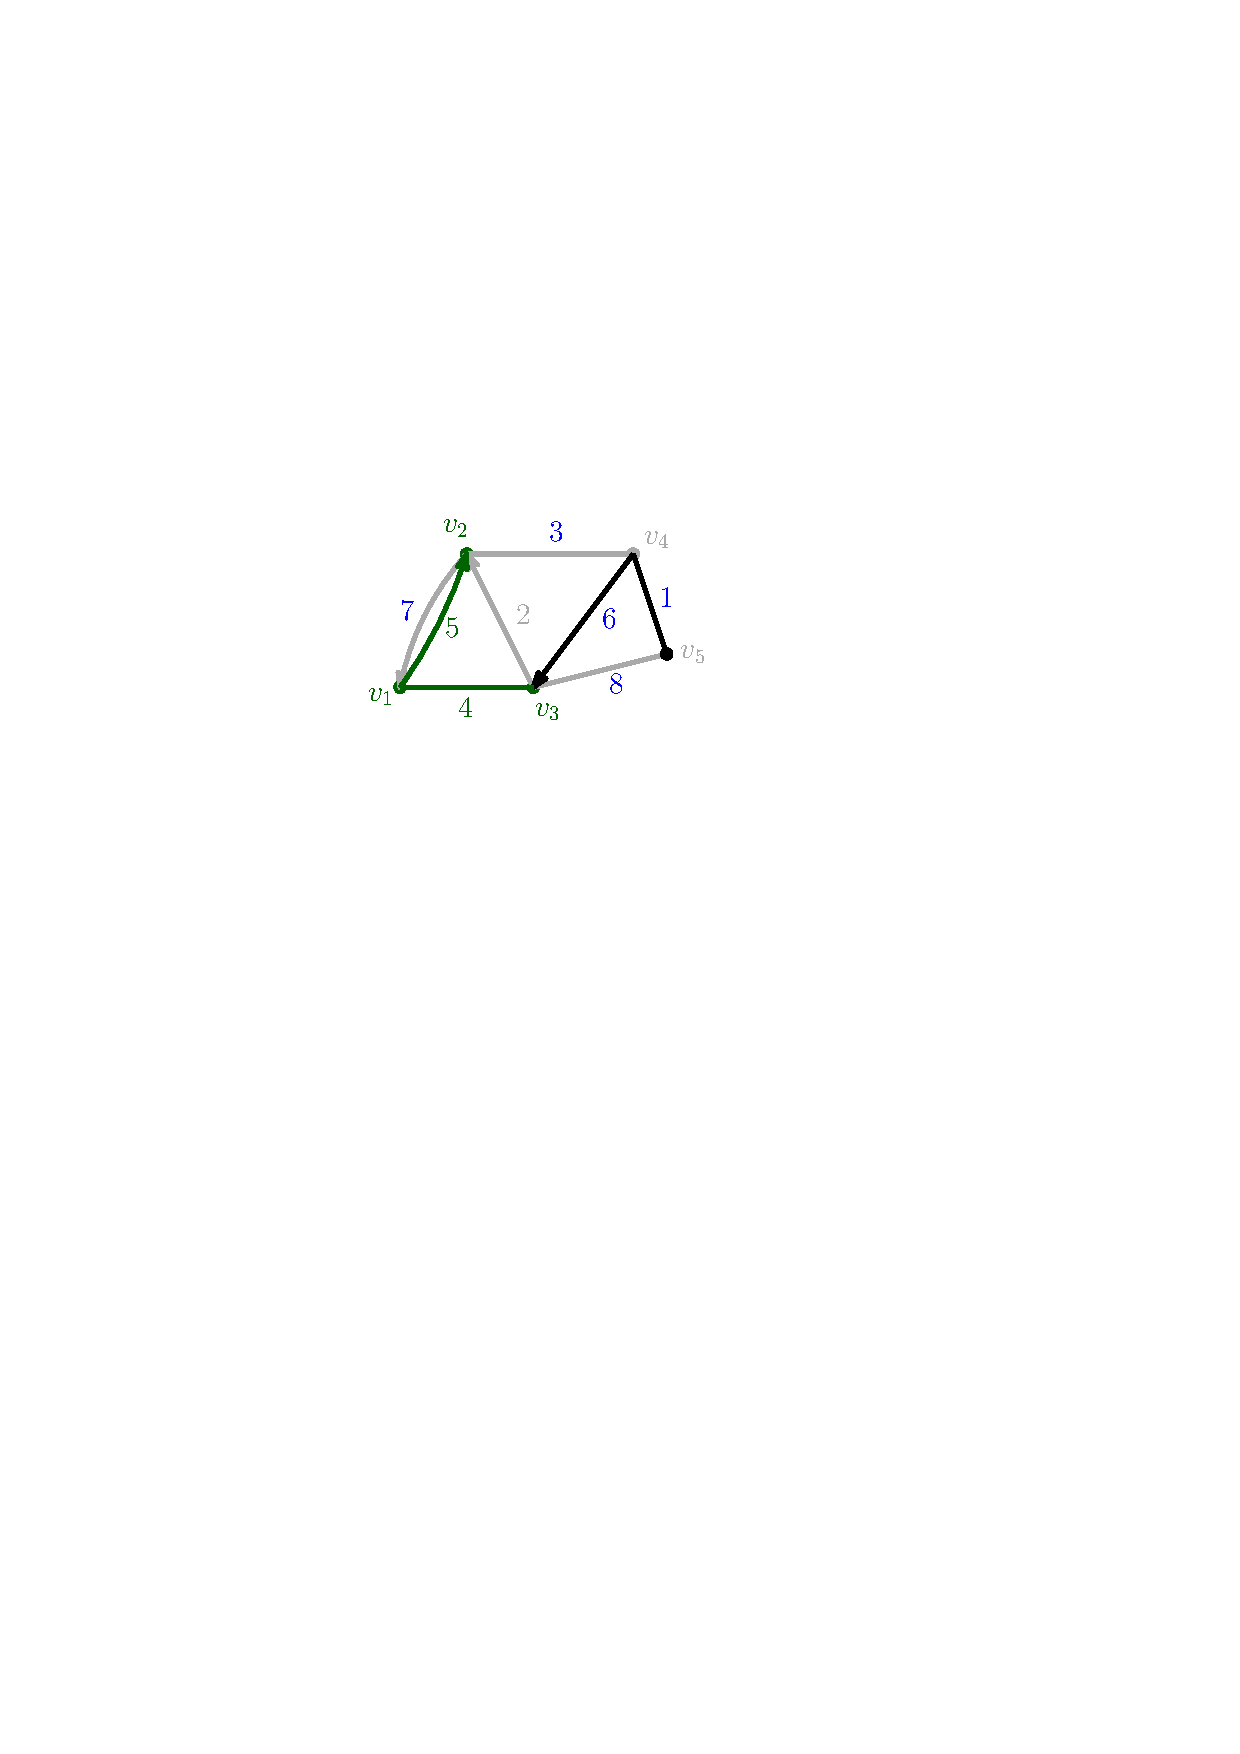
\includegraphics[width = \textwidth]{../media/dijkstra3.pdf} \\
\caption{3. Iteration}
\vspace{0.5cm}
\label{fig:dijkstra3}
\end{subfigure}
\begin{subfigure}{0.32\textwidth}
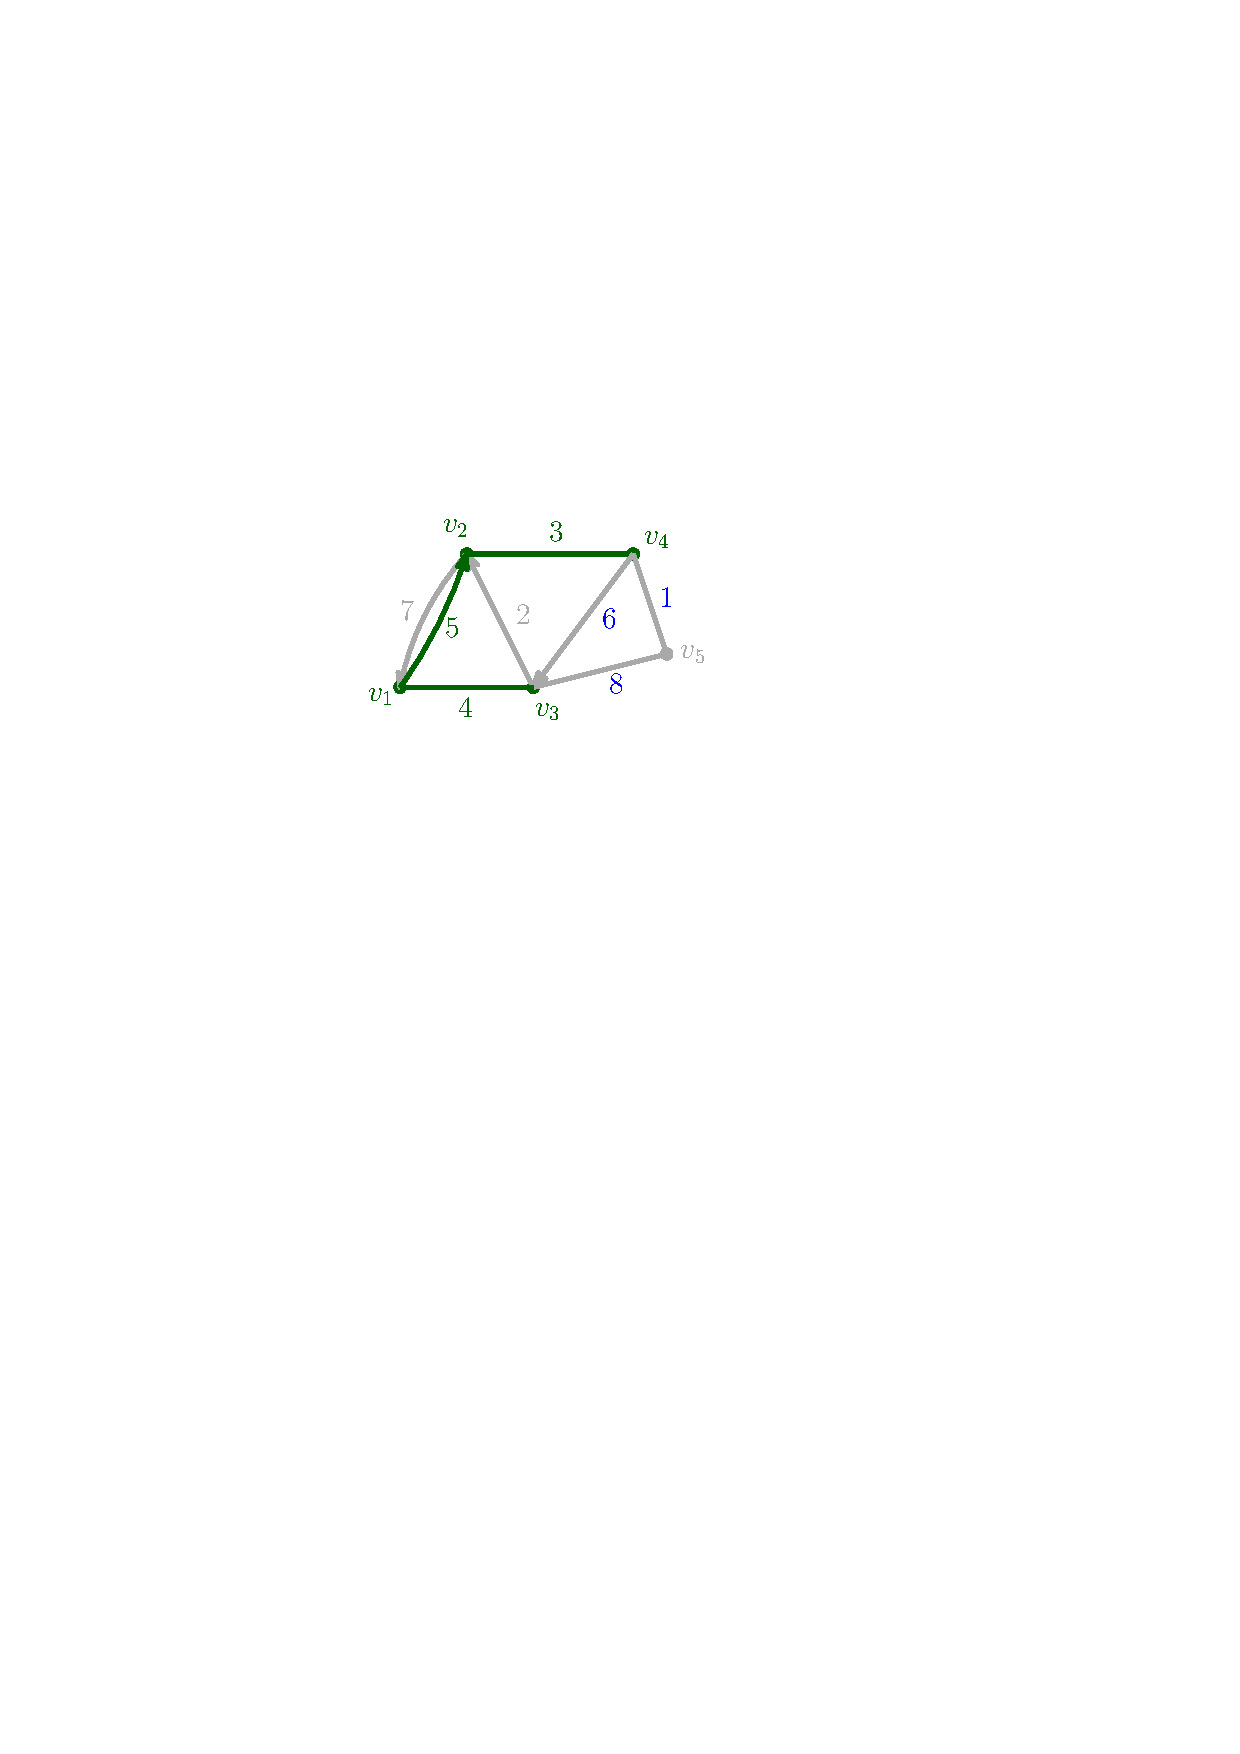
\includegraphics[width = \textwidth]{../media/dijkstra4.pdf} \\
\caption{4. Iteration}
\vspace{0.5cm}
\label{fig:dijkstra4}
\end{subfigure}
\begin{subfigure}{0.32\textwidth}
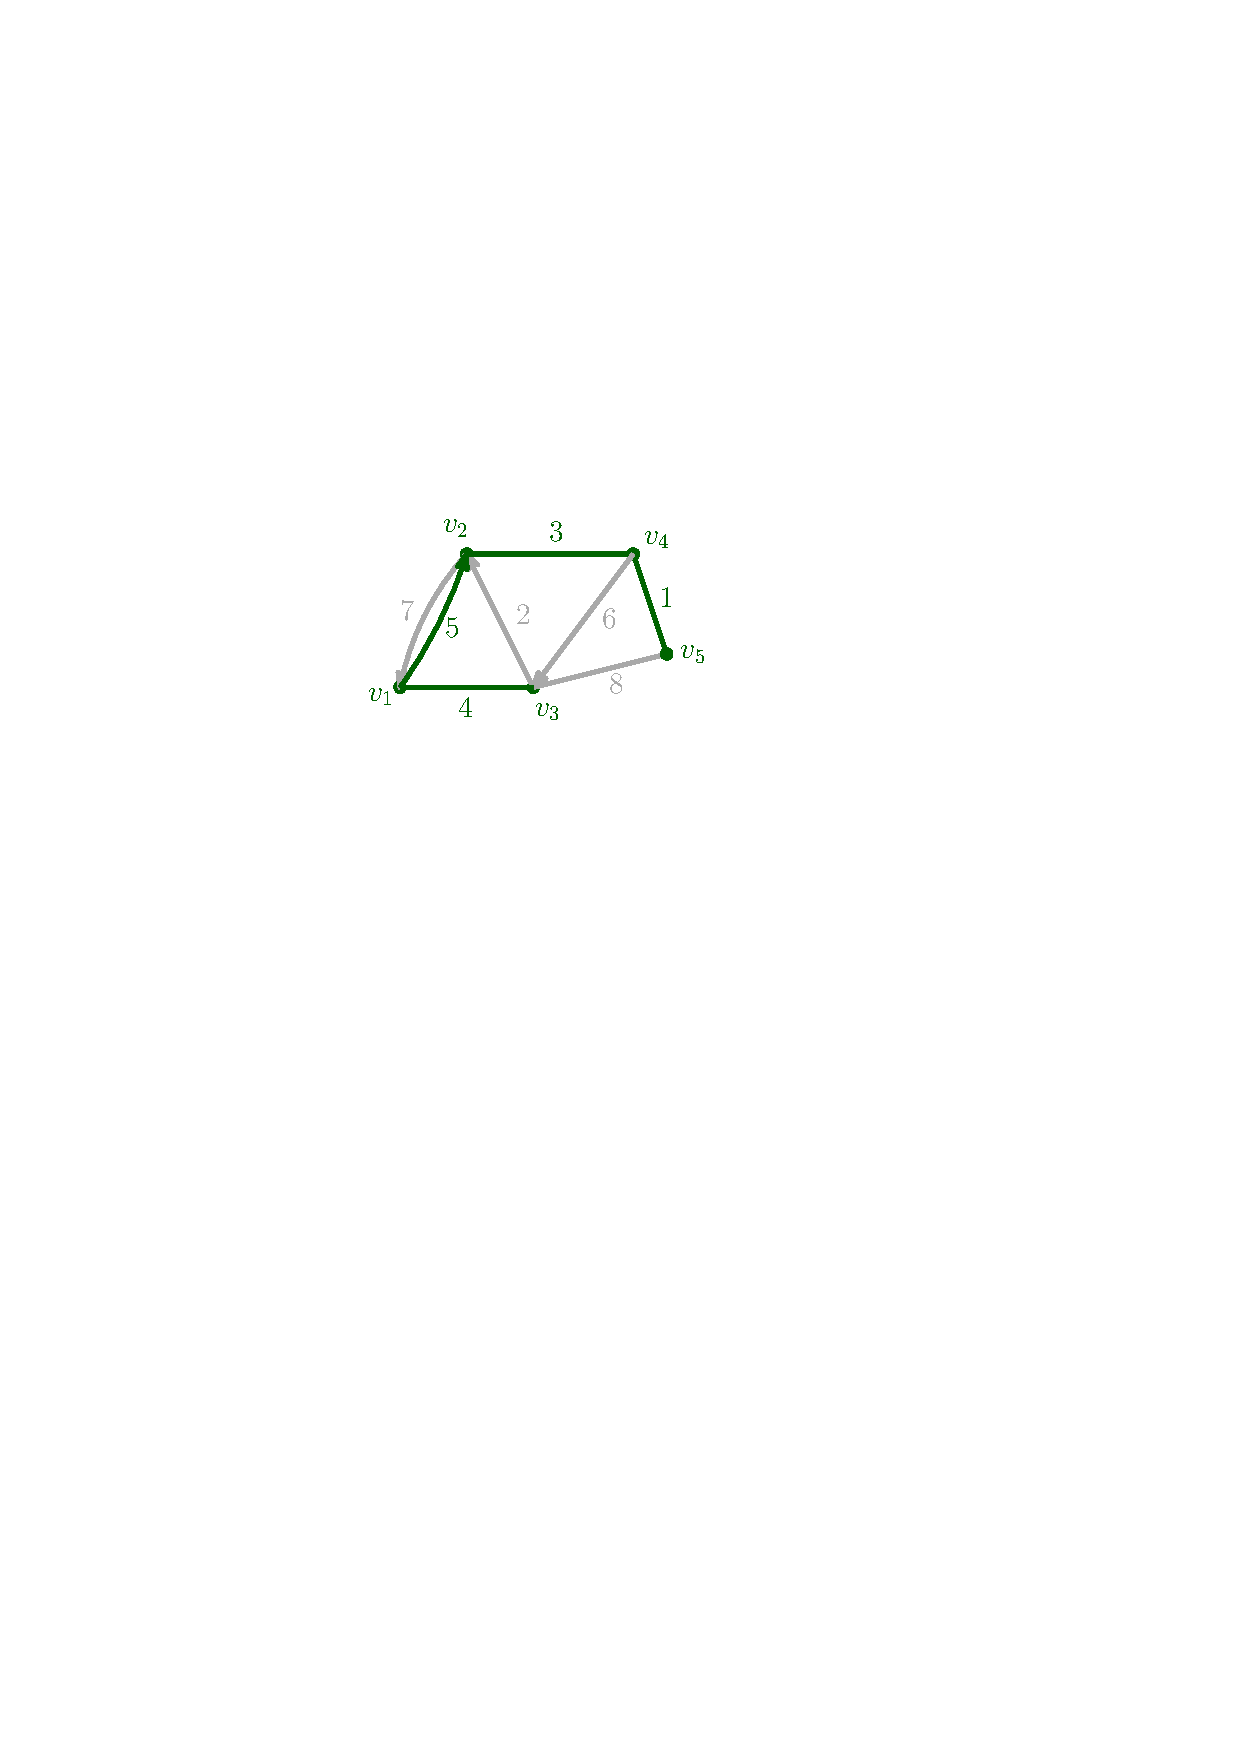
\includegraphics[width = \textwidth]{../media/dijkstra5.pdf} \\
\caption{5. Iteration}
\vspace{0.5cm}
\label{fig:dijkstra5}
\end{subfigure}
\caption{Kompletter Durchlauf eines Dijkstra Algorithmus}
\label{dijkstraIterations}
\end{figure}

\begin{table}[htb]
\centering
\label{tab:dijkstraLists}
\caption{$W_{s}$ und $K_{s}$ für jede Iteration aus Abb.~\ref{dijkstraIterations}}
\begin{tabular}{r|l|l}

\multicolumn{1}{l|}{} & \multicolumn{1}{c|}{$W_{s}$}                                                                        & \multicolumn{1}{c}{$K_{s}$}                                                                                                                                \\ \hline
1.                               & \begin{tabular}[c]{@{}l@{}}$v_{2}:5(v_{1})$ $v_{3}:4(v_{1})$\end{tabular}  & $v_{1}: 0(v_{1})$                                                                                                                    \\ \hline
2.                               & \begin{tabular}[c]{@{}l@{}}$v_{2}:5(v_{1})$ $v_{5}:12(v_{3})$\end{tabular} & \begin{tabular}[c]{@{}l@{}}$v_{1}:0(v_{1})$ $v_{3}:4(v_{1})$\end{tabular}                                                          \\ \hline
3.                               & \begin{tabular}[c]{@{}l@{}}$v_{5}:12(v_{3})$ $v_{4}:8(v_{2})$\end{tabular} & \begin{tabular}[c]{@{}l@{}}$v_{1}:0(v_{1})$ $v_{3}:4(v_{1})$ $v_{2}:5(v_{1})$\end{tabular}                                       \\ \hline
4.                               & $v_{5}:9(v_{4})$                                                           & \begin{tabular}[c]{@{}l@{}}$v_{1}:0(v_{1})$ $v_{3}:4(v_{1})$ $v_{2}:5(v_{1})$ $v_{4}:8(v_{2})$\end{tabular}                    \\ \hline
5.                               & \multicolumn{1}{c|}{-}                                                     & \begin{tabular}[c]{@{}l@{}}$v_{1}:0(v_{1})$ $v_{3}:4(v_{1})$ $v_{2}:5(v_{1})$ $v_{4}:8(v_{2})$ $v_{5}:9(v_{4})$\end{tabular} \\
\end{tabular}
\end{table}



Damit wurde das \gls{ssp} gelöst und einen kürzeste Wege zu jeder Ecke des Graphen vom Startpunkt.
Daraus ergibt sich auch die Lösung aller \gls{spp} für $s~$ zu jeder anderen Ecke aus $V~$.
Es ist jedoch nicht sinnvoll für die Lösung eines \gls{spp} jedes mal das \gls{ssp} für den kompletten Graphen zu berechnen.
Das liefert nicht nur viele irrelevante Ergebnisse sondern kostet auch mehr Berechnungsressourcen und Zeit.
Daher gibt es unterschiedliche Möglichkeiten den Dijkstra Algorithmus zu beschleunigen.

\subsubsection{Speedup Techniken}

\paragraph*{Early Stopping:}
Der Algorithmus wird bisher jedes mal für den ganzen Graphen ausgeführt, obwohl oft nur die Route für einen kleinen Bruchteil des Graphen benötigt wird.
Die einfachste Methode ist den Dijkstra zu stoppen, nachdem $z~$ erreicht wurde (~\ref{fig:normalD}).

\paragraph*{Bidirectional Dijkstra:}
Beim \textit{Bidirectional Dijkstra} werden zeitgleich zwei Algorithmen nebeneinander ausgeführt.
Einer auf $s~$ und einer auf $z~$ (auf einem umgekehrt gerichteten Graphen).
Für beide Instanzen gibt es eine separate Warteschlange $W_{s}$ und $W_{z}$.
Zu Beginn wird für jeden Startpunkt die initiale der umliegenden Ecken durchgeführt.
Anschließend wird die Ecke mit der geringsten Distanz in beiden Warteschlangen markiert und aus der jeweiligen Warteschlange entfernt.
Wird eine Ecke aus beiden Warteschlangen entfernt, werden $W_{s}$ und $W_{z}$ auf weitere übereinstimmende Ecken geprüft.
Für jede Übereinstimmung wird die Distanz in beiden Instanzen Berechnet.
Die Ecke ist Teil des kürzesten Weges wenn die Summe beider Distanzen minimal ist.\par
In der schematischen Abbildung ~\ref{fig:biD} wird die Einsparung gegenüber dem Early Stopping deutlich.
Der graue Bereich muss nicht berechnet werden.
Die Bearbeitungszeit lässt sich also theoretisch um die Hälfte reduzieren\footnote{In der Realität wird dieser Wert selten erreicht.
Bei Graphen mit einer höheren Eckendichte in Nähe von $z~$ könnte die Bearbeitungszeit sogar größer werden.
Allgemein wird aber ein signifikanter Vorteil erzielt.}.

\begin{figure}[htb]
\centering
\begin{subfigure}{0.30\textwidth}
\centering
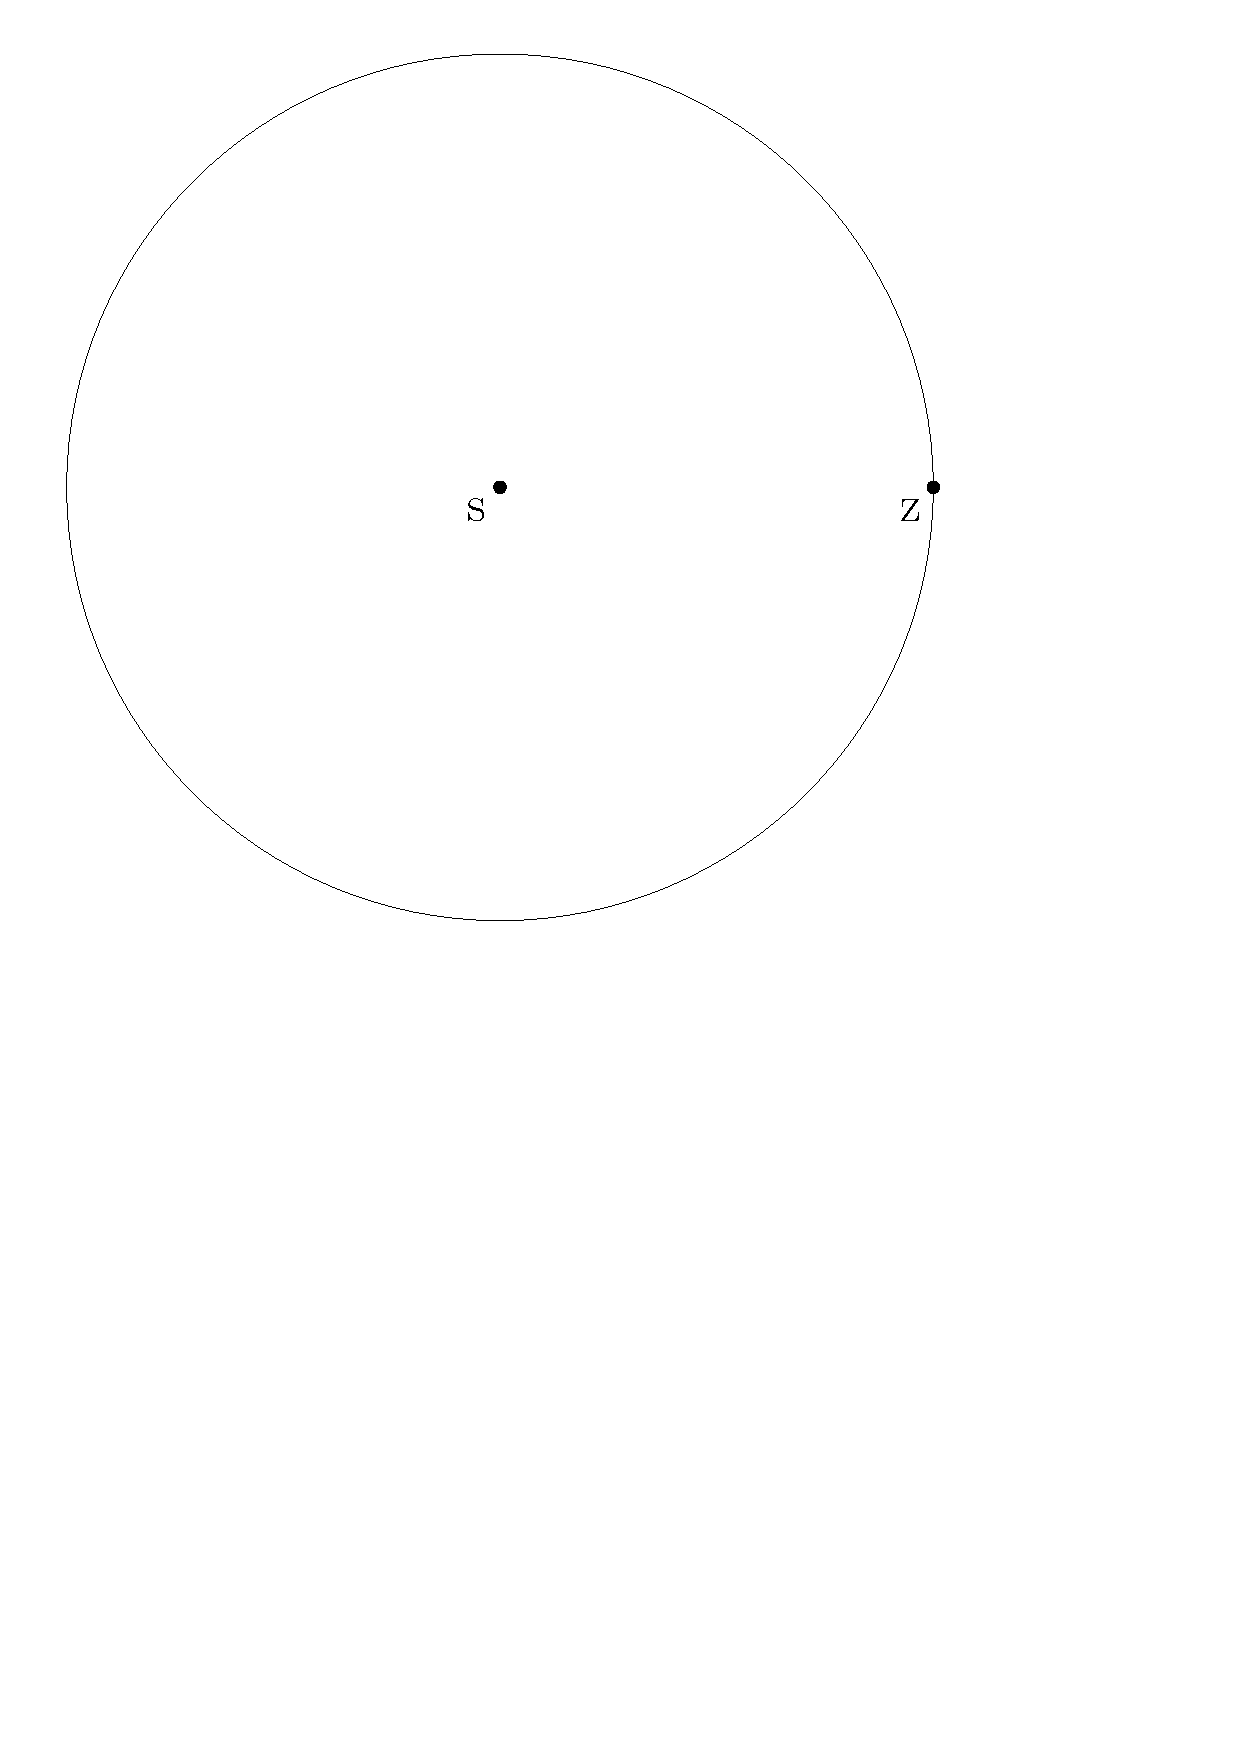
\includegraphics[width = \textwidth]{../media/normaldijkstra.pdf} \\
\caption{Early Stopping}
\label{fig:normalD}
\end{subfigure}
\begin{subfigure}{0.30\textwidth}
\centering
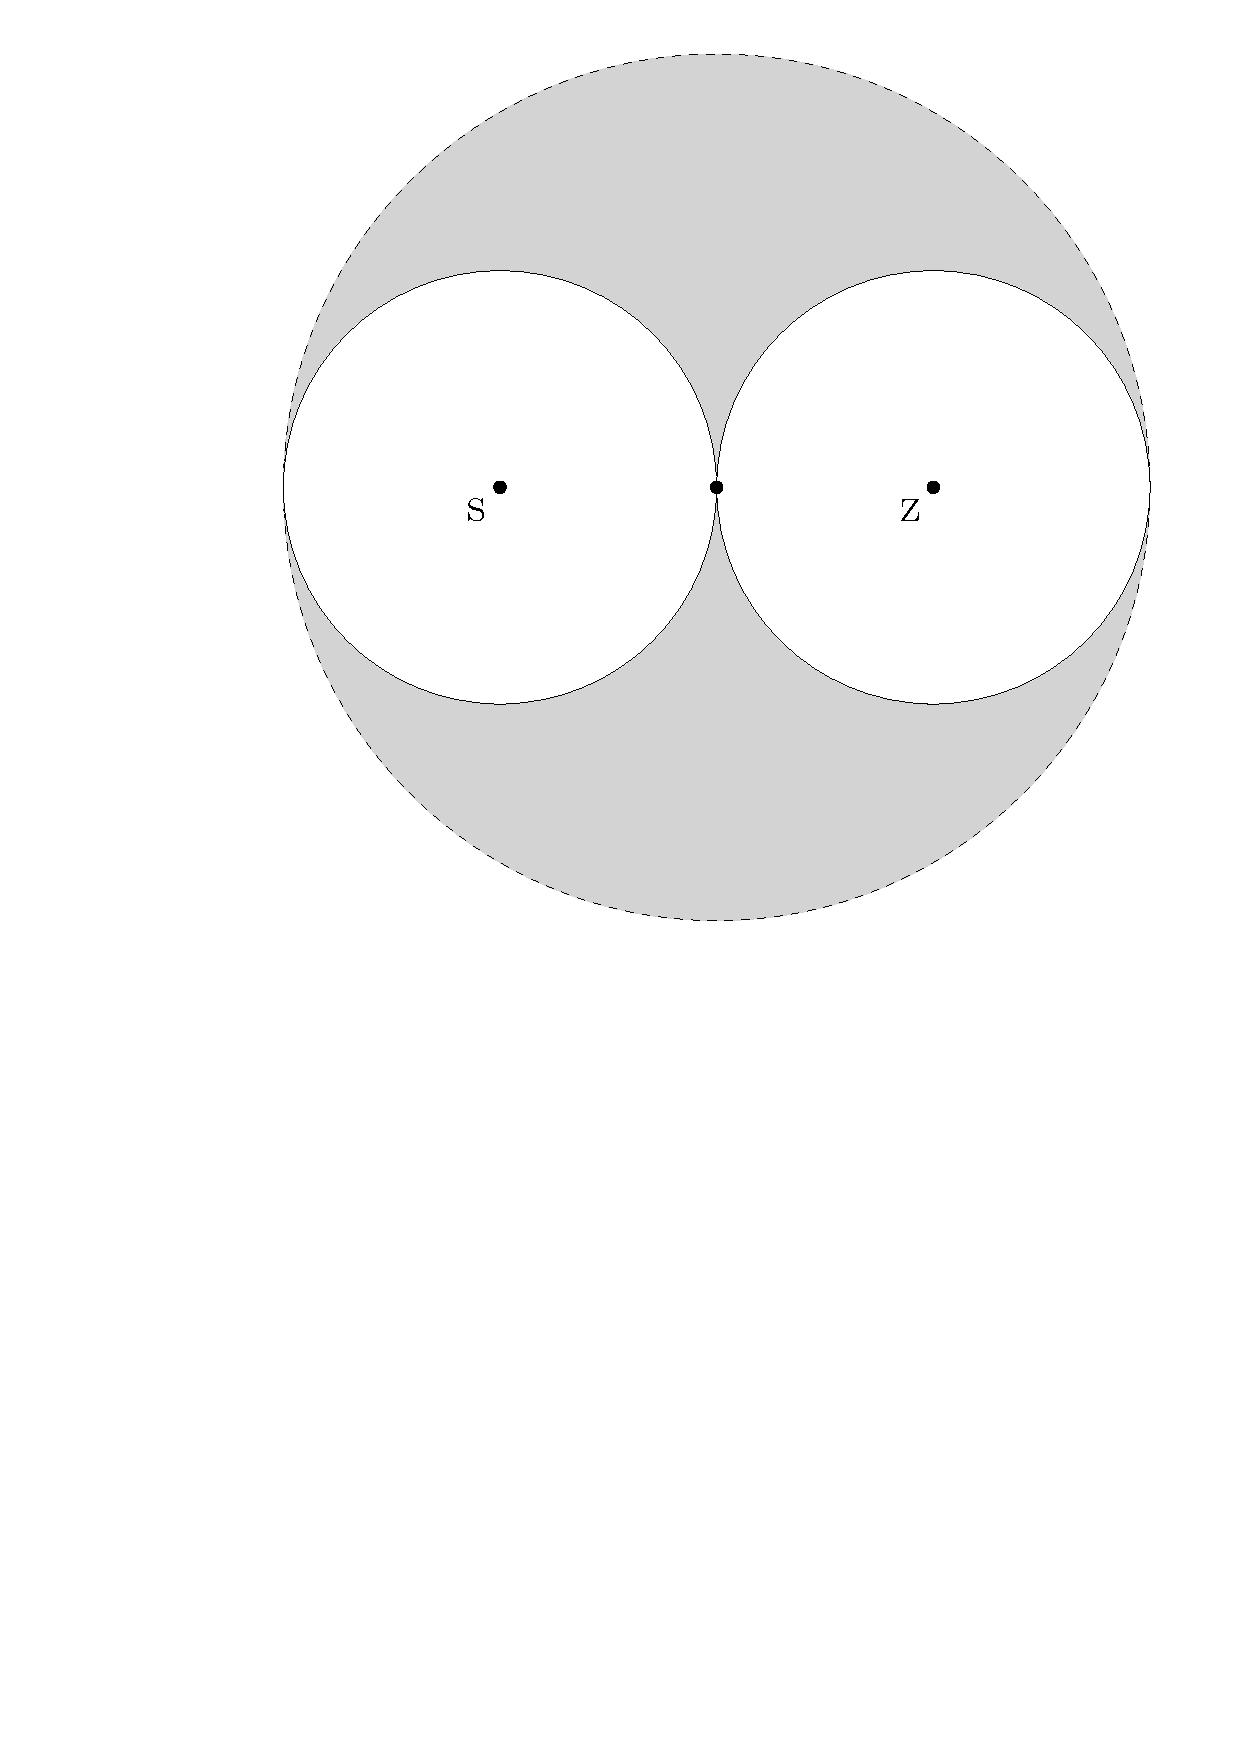
\includegraphics[width = \textwidth]{../media/bidijkstra.pdf} \\
\caption{Bidirectional D.}
\label{fig:biD}
\end{subfigure}
\begin{subfigure}{0.30\textwidth}
\centering
\vspace{1.1cm}
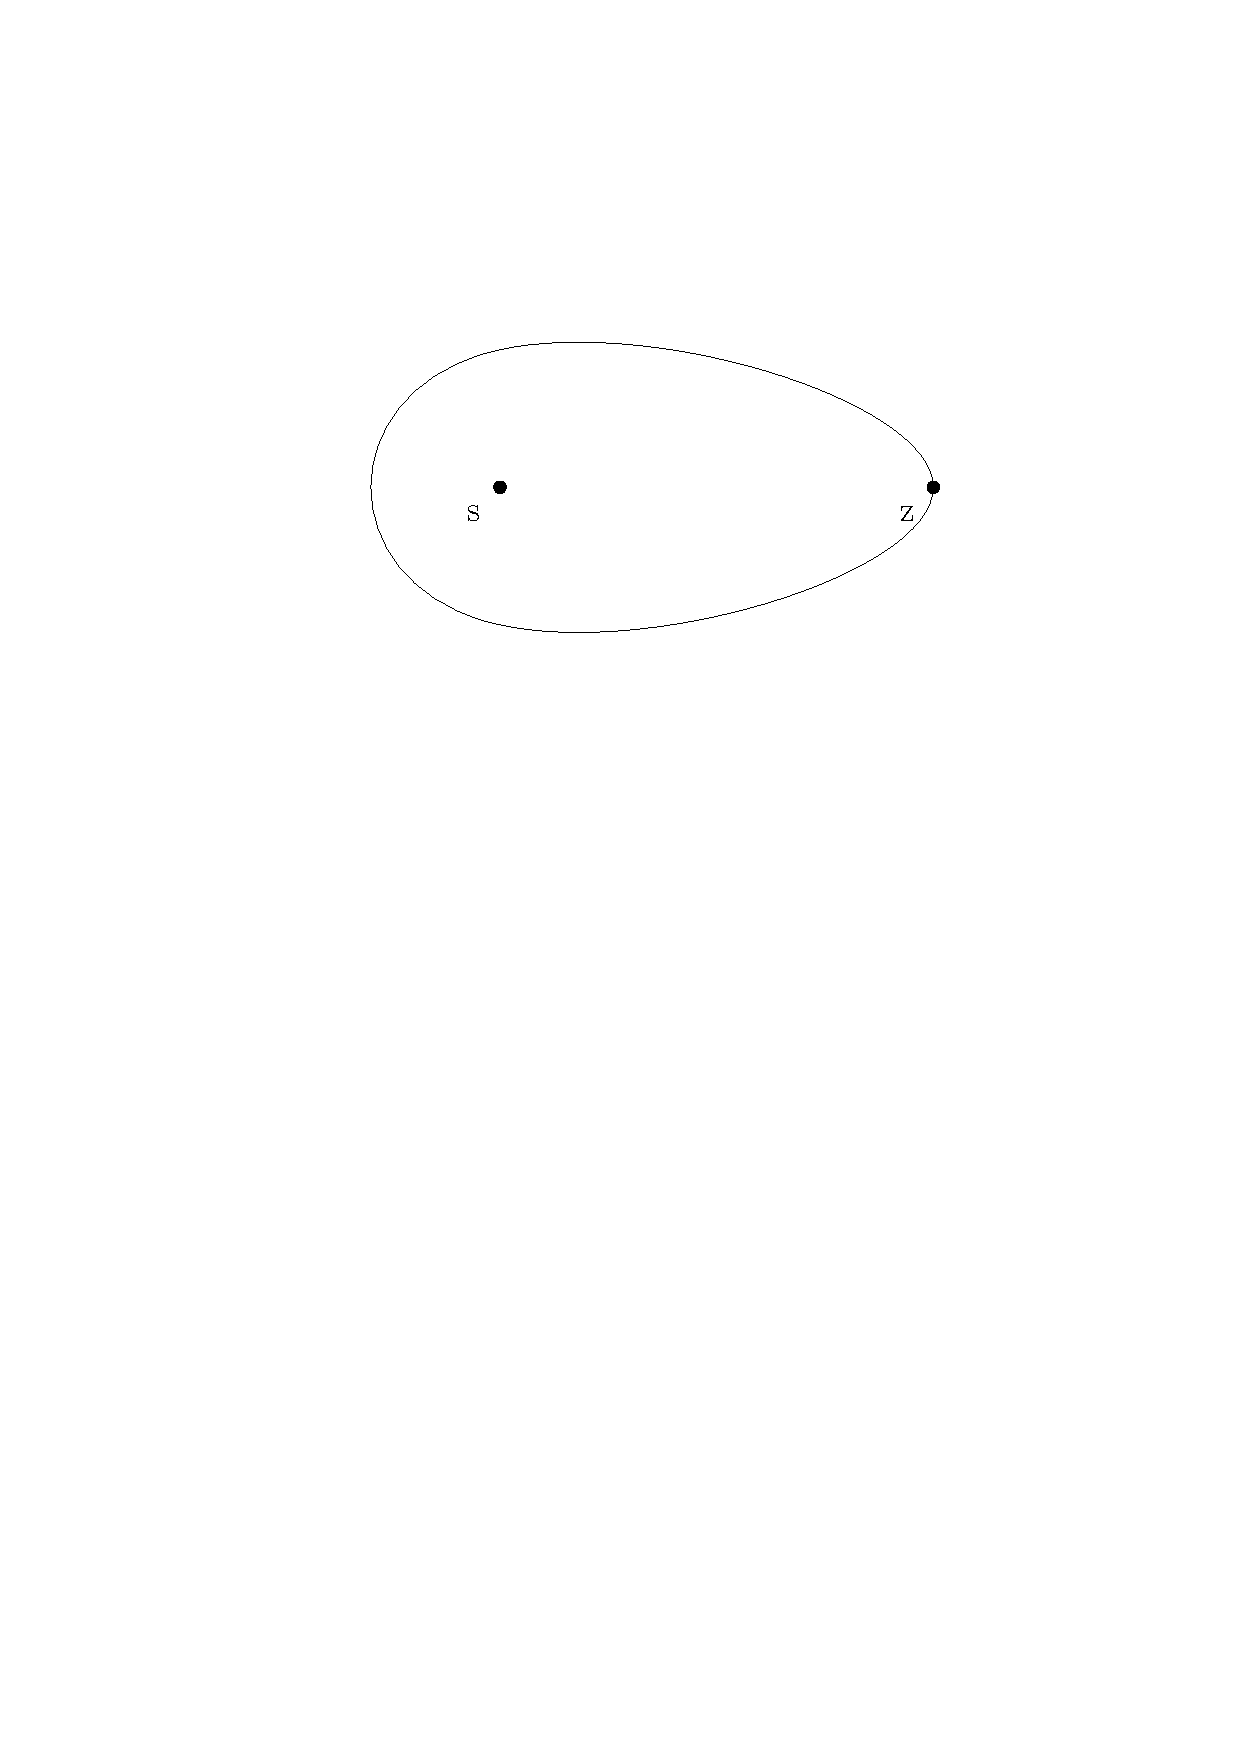
\includegraphics[width = \textwidth]{../media/stardijkstra.pdf} \\
\vspace{0.9cm}
\caption{A*}
\label{fig:starD}
\end{subfigure}
\caption{Speedup Techniken für den Dijkstra Algorithmus}
\label{speedup}
\end{figure}


\paragraph*{A*:}
Der $A*~$Algorithmus ist eine Variante des Dijkstras die den Suchraum in Richtung der Zielecke lenkt.
Es wird durch eine Funktion für jede Ecke die Distanz zum Ziel geschätzt.
Diese wird mit den Kantengewichten verrechnet damit Ecken in Zielrichtung früher markiert werden.
Die standardmäßig kreisförmige Ausbreitung des Dijkstras wird mit dem A* zu einem Oval gestreckt.
Da der Zielpunkt so früher erreicht wird, müssen weniger Iterationen durchgeführt werden.

Diese und weitere Möglichkeiten sind in \cite[209--213]{kurt} ausführlich beschrieben.

\subsection{Isochronen Berechnung}

Isochronen sind Linien gleicher Zeit (griech.: \textit{iso} = gleich + \textit{chronos} = Zeit).

Wenn in einem gewichteten Graphen die Kanten die benötigte Zeit enthalten, um von einer Ecke zur nächsten zu gelangen, können damit Analysen zur Erreichbarkeit durchgeführt werden.
Dazu wird ein \gls{ssp} für eine zentrale Ecke~$z$ mit einem gegebenen Zeitlimit~$t$ gelöst.
Isochronen können mit unterschiedlichen Methoden berechnet werden.
Das resultierende Objekt ist immer ein Polygon, welches jeden in gegebenem Zeitlimit erreichbaren Punkt beinhaltet.


\subsubsection{Gitterbasierter Ansatz}

Beim \textit{Marching Squares} Algorithmus wird um das Zentrum ein Gitter über dem Graphen gebildet~(\ref{fig:grid1}).
Die Eckpunkte des Gitters erhalten dabei die Werte des nächsten Punktes auf dem Graphen~(\ref{fig:grid2}).
Anschließend werden auf den Kanten des Gitters diejenigen Punkte markiert, bei denen der Wert mit dem gesuchten Zeitlimit übereinstimmt.
In Abbildung~\ref{fig:grid3} wurde das für die Werte $t=5$ und $t=10$ durchgeführt.
Die markierten Punkte werden verbunden und bilden schließlich die Isochrone.

\begin{figure}[htb]
\centering
\begin{subfigure}{0.47\textwidth}
\centering
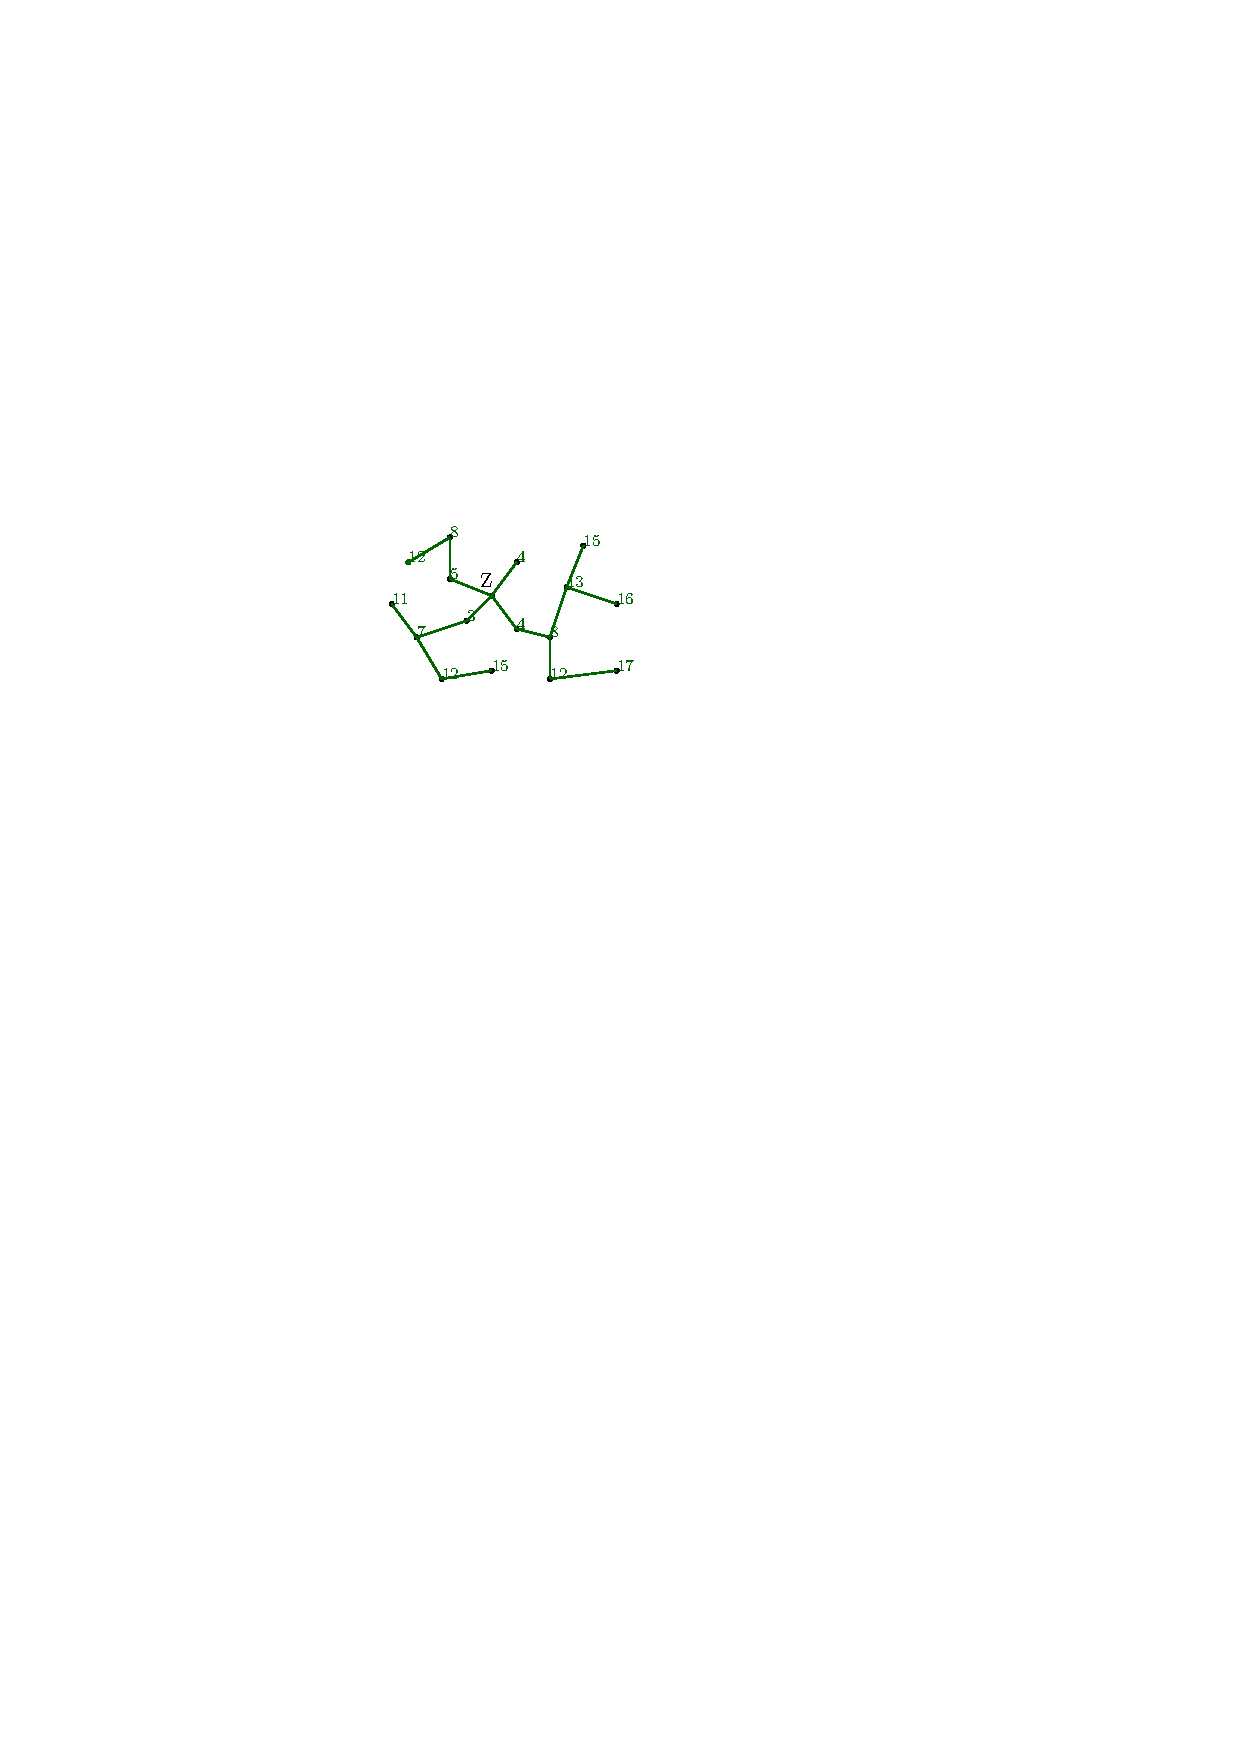
\includegraphics[width = \textwidth]{../media/grid.pdf} \\
\caption{Basis Graph mit kürzesten Wegen}
\vspace{0.3cm}
\label{fig:grid1}
\end{subfigure}
\begin{subfigure}{0.47\textwidth}
\centering
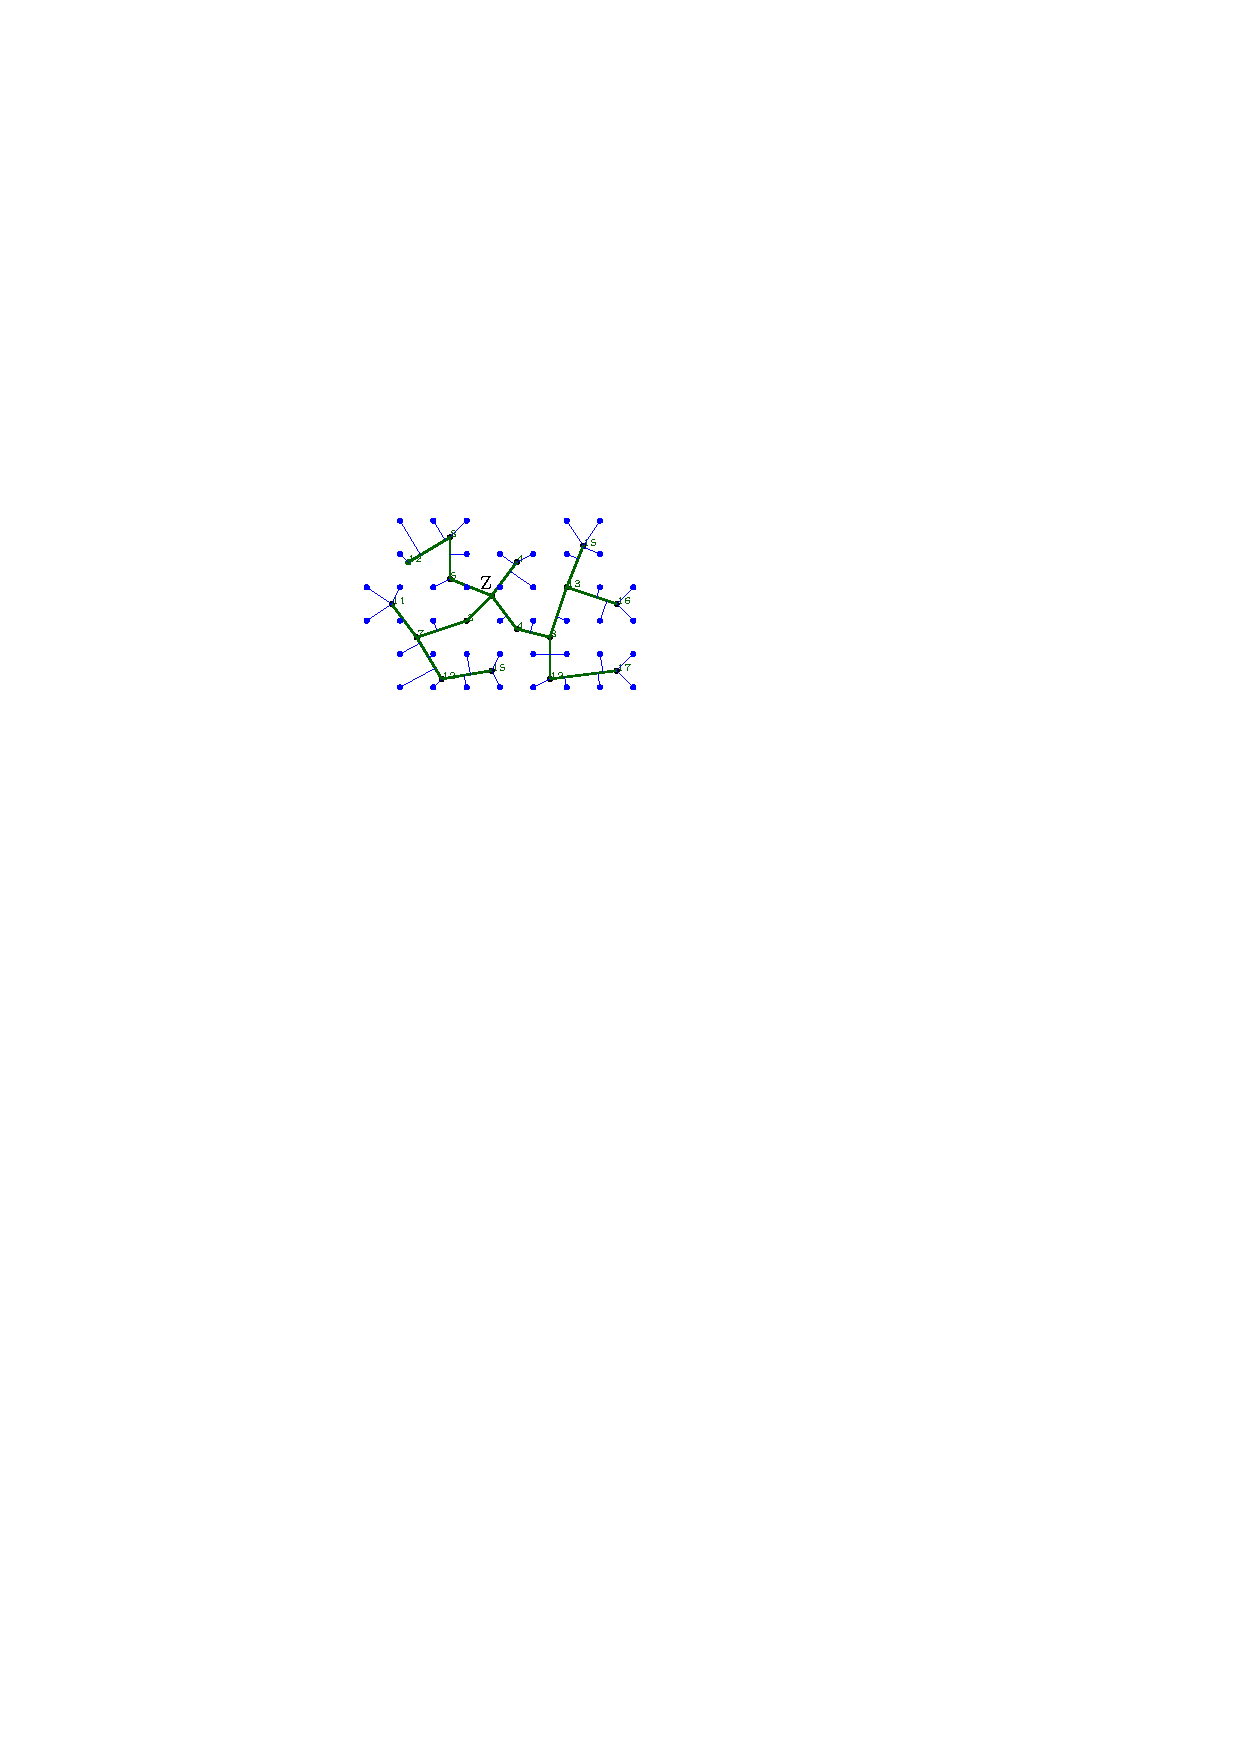
\includegraphics[width = \textwidth]{../media/gridsnap.pdf} \\
\caption{Gitterbildung}
\vspace{0.3cm}
\label{fig:grid2}
\end{subfigure}
\begin{subfigure}{0.44\textwidth}
\centering
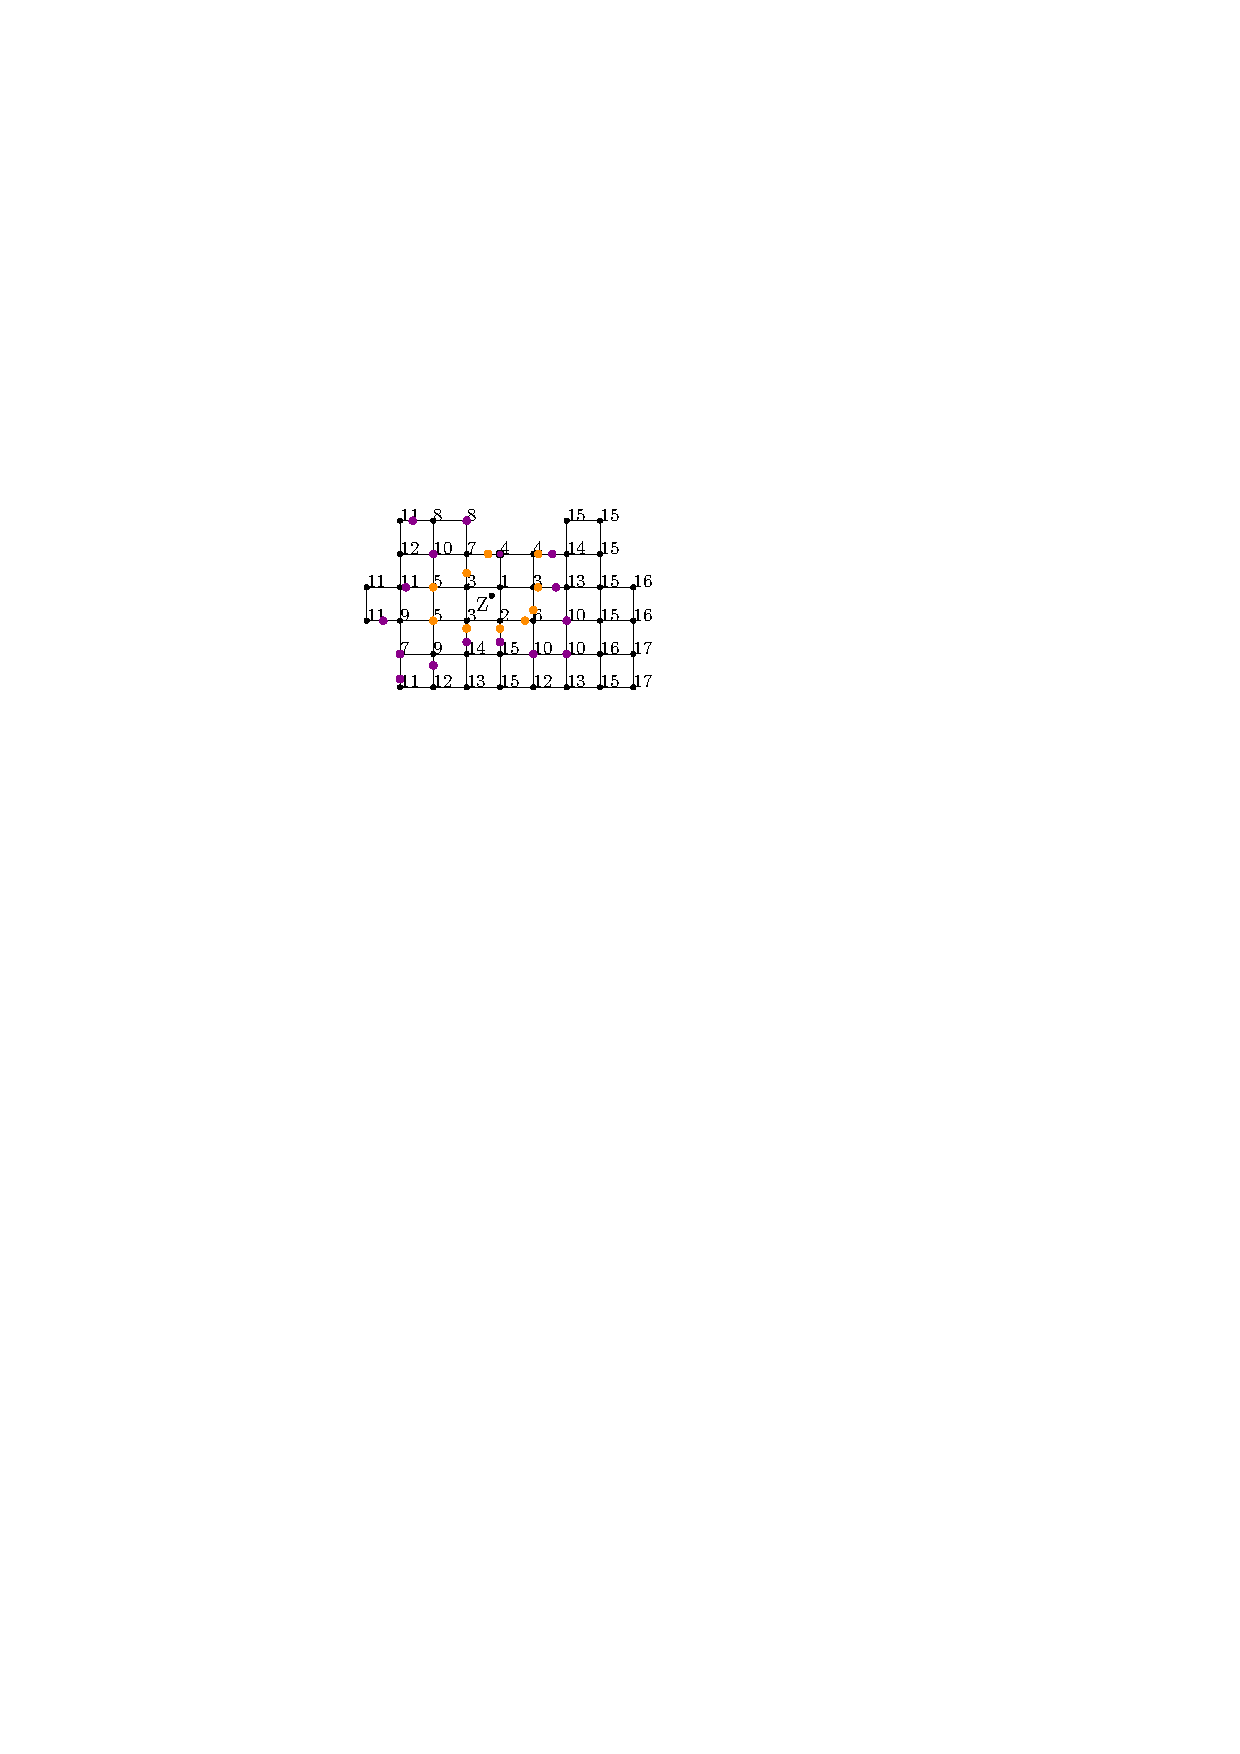
\includegraphics[width = \textwidth]{../media/gridedge.pdf} \\
\caption{Kantenmarkierung}
\label{fig:grid3}
\end{subfigure}
\begin{subfigure}{0.47\textwidth}
\centering
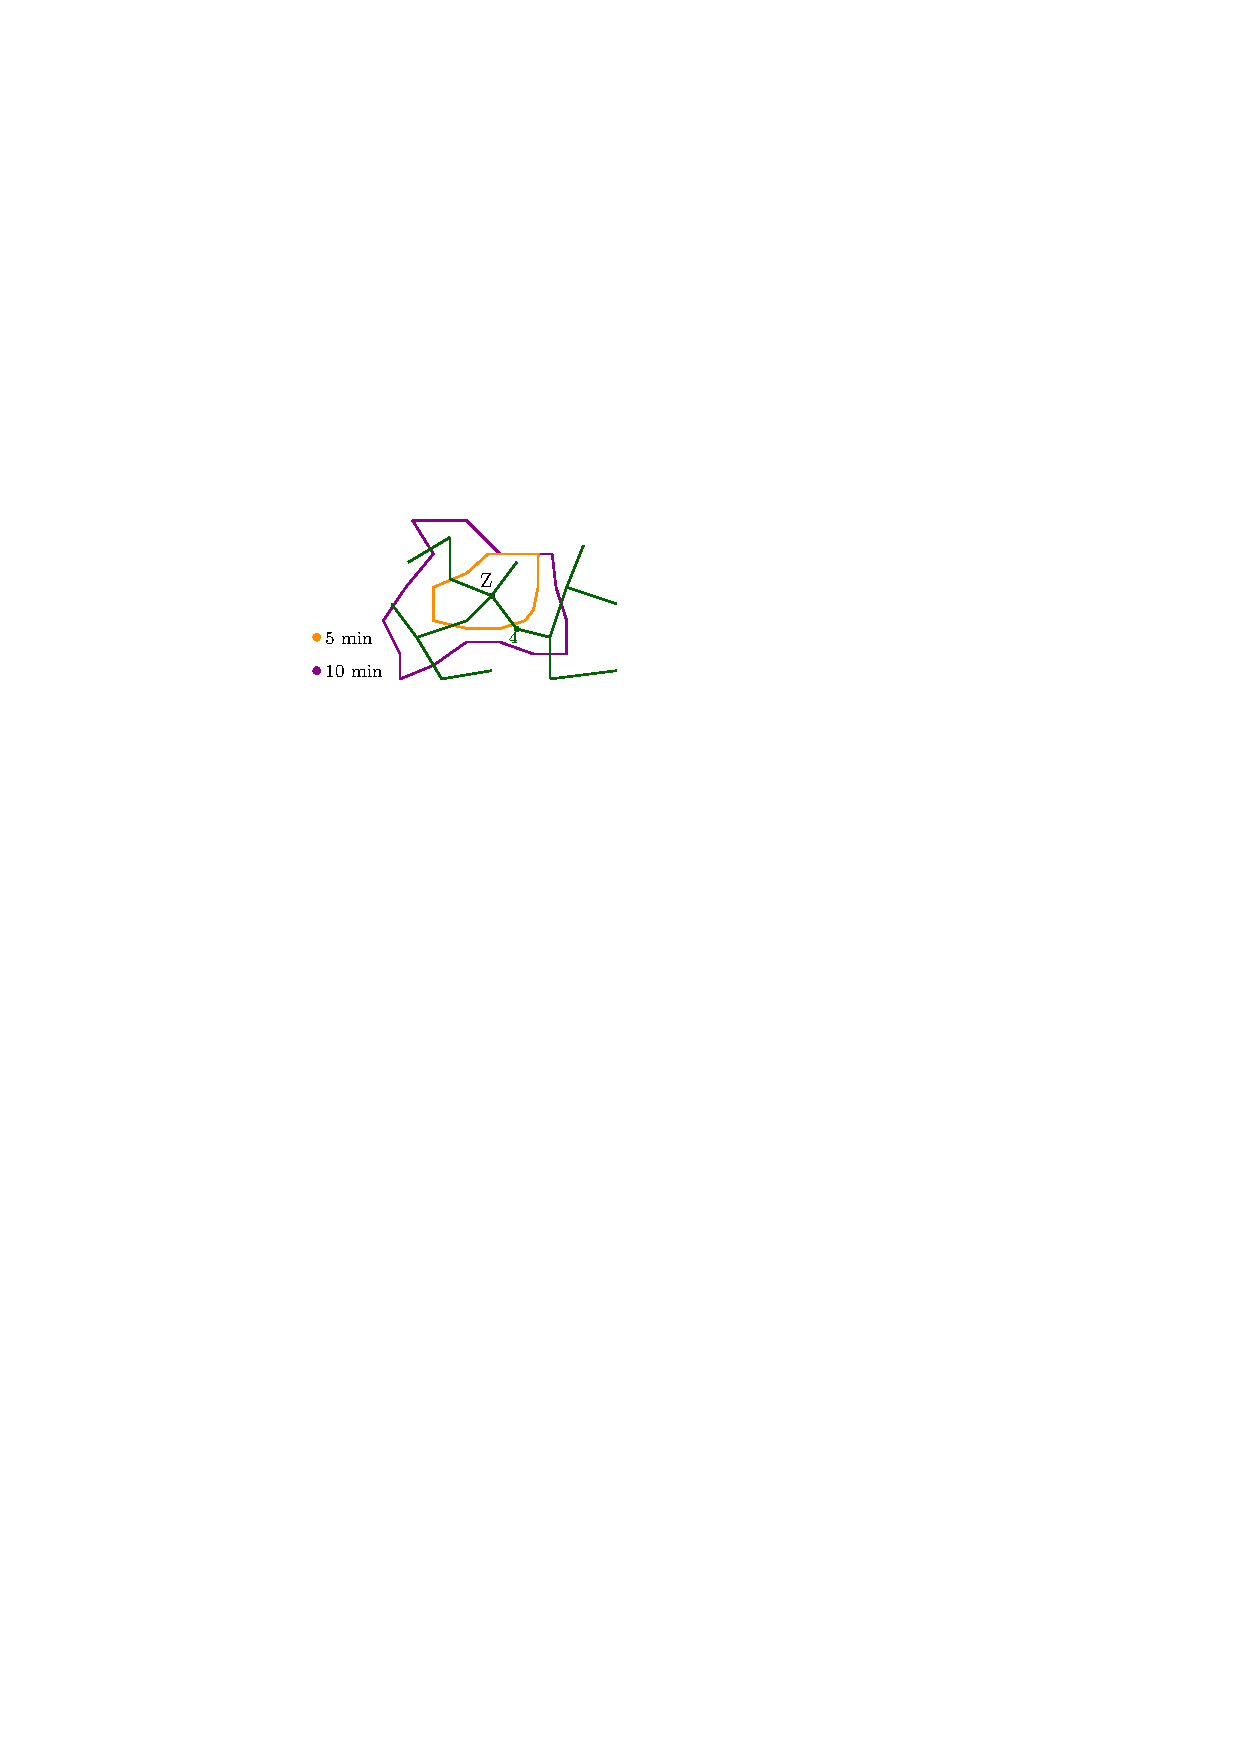
\includegraphics[width = \textwidth]{../media/gridiso.pdf} \\
\caption{Resultierende Isochrone}
\label{fig:grid4}
\end{subfigure}
\caption{Marching Squares Algorithmus}
\label{grid}
\end{figure}

Der Vorteil dieses Algorithmus ist, dass die Maschengröße des Gitters angepasst werden kann.
Bei sehr kleinen Maschen liefert der Algorithmus ein sehr genaues Ergebnis.
Allerdings werden dabei mehr Ressourcen zur Berechnung benötigt.
Daher sollten lediglich kleine Gebiete sowie geringe Zeitbeschränkungen berechnet werden.
Bei weiten Maschen ist der Algorithmus dagegen sehr schnell und kann größere Distanzen und längere Zeitspannen berechnen.
Das Ergebnis ist dementsprechend aber auch ungenauer.
In Abbildung ~\ref{fig:grid4} wurde die Größe der Maschen beispielsweise ungeschickt gewählt, da eine Ecke mit Abstand vier Minuten vom Zentrum liegt und dadurch außerhalb der fünf-Minuten-Isochrone.

\subsubsection{Dreiecksvermaschung}
\cite{isochrones} beschreiben eine anschauliche Methode um Isochronen zu berechnen.
Nach der Lösung des \gls{ssp}s werden den Ecken des Graphen der geographischen Koordinate der repräsentierten Kreuzung zugeteilt.
Die Kanten werden nicht benötigt und daher entfernt.
Es liegt demnach eine 3D-Punktwolke vor.
Jeder Ecke wird nun die benötigte Zeit zugewiesen, mit der diese zu erreichen ist.
Anschließend werden die Ecken nach dem Delaunay Triangulationsverfahren vermascht.
Dadurch entsteht eine Art Trichter mit der Startecke als Tiefpunkt auf der Höhe Null.
Wird dieser Trichter auf Höhe des Zeitlimits geschnitten, entsprechen von oben betrachtet die Randkanten des Trichters der Isochrone.


\subsubsection{Formenbasierter Ansatz}
\label{sec:form}
Die Implementierung des \gls{ors} zur Berechnung von Isochronen verwendet einen Form-basierten Ansatz.
Zuerst werden mit dem in Kapitel ~\ref{sec:dijkstra} bereits ausführlich erklärten Dijkstra Algorithmus alle in gegebener Zeit erreichbaren Kanten markiert.
Anschließend werden die geographischen Punkte (Pillar Nodes) aus der $WayGeometry$ der Kante extrahiert (Siehe Kapitel ~\ref{sec:osmgraph} auf Seite ~\pageref{sec:osmgraph}).
Um jeden der extrahierten Punkte wird ein kreisförmiger Pufferbereich gelegt.
Dadurch können nahe beieinanderliegende Punkte übersprungen werden.
Mit den verbleibenden Punkten wird eine Punktwolke generiert.
Auf dieser Punktwolke wird nun der Alpha-Shape Algorithmus (\cite{akkiraju1995alpha}) angewandt, um die Isochrone als Hülle um die erreichbaren Wegsegmente zu zeichnen.
%\todo{(Abb. Pictures shape based stuff)}
Dieser Ansatz liefert präzise Ergebnisse bei schnellen Berechnungszeiten.
Die Verwendung der Alpha-Shapes verhindert allerdings die Möglichkeit der Darstellung von nicht erreichbaren Gebieten innerhalb der Isochronen.


\newpage

\section{Methodik}
Die grundsätzlichen Überlegungen beruhen, wie in der Einleitung bereits erwähnt, auf den Notstandsvollmachten durch §35 Absatz 1 der StVO für Einsatzfahrzeuge des Rettungsdienstes, der Feuerwehr und der Polizei.
Demnach dürfen sich Einsatzfahrzeuge im Notfall über die Vorschriften der StVO hinwegsetzen.

Die Frage, die sich hierbei stellt, ist, inwieweit von diesen Rechten im Ernstfall Gebrauch gemacht werden kann.
Um diesen Sachverhalt zu untersuchen, wurde ein Fragenkatalog für die \gls{ffl} zusammengestellt.
Dieser wurde als Datei in der Cloud gespeichert und ist auch weiterhin verfügbar (Link im Anhang auf S.\pageref{sec:anhang}).
Die Fragen wurden unter Berücksichtigung der \gls{osm}-Datenstruktur und des vorhandenen \gls{ors}-Backend gewählt.
Die Antworten der \gls{ffl} sind hier sinngemäß wiedergegeben und die wörtlichen Antworten sind dem Cloud-Dokument im Anhang zu entnehmen.
Auf Basis der erhobenen Informationen wurden geeignete \gls{osm}-Tags gesucht, mit denen die empfohlenen Änderungen verwirklicht werden können.
Anschließend wurden neue Java-Funktionen geschrieben, um diese Tags bei der Erstellung des Graphen und bei Anfragen zu berücksichtigen.
Außerdem wurde das Frontend an das neue Profil angepasst.

\subsection{Informationserhebung}

\paragraph*{1. Maße der Fahrzeuge:}
\label{frage1}
\par
Die Dimensionen des Fahrzeuges sind limitierende Faktoren für bestimmte Wegsegmente.
Manche Brücken halten nur ein bestimmtes Gewicht aus und ein Tunnel hat nur eine gewisse Höhe.
Hier stützt sich das \gls{ors}-Backend auf Restriktionen durch die \gls{osm}-Tags: \texttt{maxlength, maxwidth, maxheight, maxweigth} und \texttt{maxaxleload} Von der \gls{ffl} wurde als wichtigstes Fahrzeug Löschfahrzeuge der Klasse LF8, LF8/6 und MLF mit folgenden Daten angegeben:
\begin{itemize}
\centering
\item[Länge:] 7 Meter
\item[Breite:] 2,5 Meter
\item[Höhe:] 3 Meter
\item[Gewicht:] 7,5 Tonnen
\end{itemize}

\paragraph*{2. Maximale Geschwindigkeiten auf unterschiedlichen Straßentypen:}
\label{frage2}
\par
Es kann nicht auf jeder Straße mit maximaler Geschwindigkeit des Fahrzeugs gefahren werden.
Deswegen werden für jede Kante des Graphen Geschwindigkeitsmaxima definiert.
Dabei wird auf einen Standardwert für den Straßentyp, die \textit{Values} (Werte) des \gls{osm} \textit{Keys} (Schlüssel) \texttt{highway}, zurückgegriffen.
Tabelle \ref{tab:speedinfo} zeigt die bisherigen Standardgeschwindigkeiten für das Heavy-Vehicle(\textit{dt.:Schwerfahrzeug})-Profil des \gls{ors}, zusammen mit den vorgeschlagenen Werten der \gls{ffl} in Klammer.
Es wurde darauf hingewiesen, dass die 80km/h auf Autobahnen nur gelten, wenn kein Stau besteht.
Im Fall eines Staus wäre laut \gls{ffl} auch die Anfahrt auf der Gegenfahrbahn bzw. entgegen der Verkehrsrichtung auf der gleichen Bahn interessant.

Genaue Informationen zu einzelnen Tags können der \gls{osm}-Wikipedia (\cite{osmwiki}) entnommen werden.

\begin{table}[htb]
\centering
\caption{Standardgeschwindigkeiten für unterschiedliche \texttt{highway} Values}
\label{tab:speedinfo}
\begin{tabular}{|l|r|}
\hline
\multicolumn{1}{|l|}{\texttt{highway} Value} & \multicolumn{1}{c|}{\textit{km/h}} \\
\hline
\multicolumn{2}{|l|}{\textit{Autobahnen}} \\
\hline
motorway (Autobahn) & 80 \\
motorway\_link (Autobahn-Zubringer) & 50 \\
motorroad (Kraftfahrtstraße) & 80 \\
trunk (Schnellstraße) & 80 \\
trunk\_link (Zubringer zu Schnellstraße) & 50 \\
\hline
\multicolumn{1}{|l}{\textit{Siedlungen}} & \multicolumn{1}{l|}{ } \\
\hline
primary (Bundesstraßen) & 60(80) \\
primary\_link  & 50 \\
secondary (Landes-/Staatsstraßen) & 60(80) \\
secondary\_link  & 50 \\
tertiary (Kreisstraßen) & 60(80) \\
tertiary\_link  & 50 \\
unclassified (Nebenstraße (oft ohne Mittellinie))  & 60 \\
residential (Straße an und in Wohngebieten) & 50 \\
living\_street (Spielstraße)  & 10 \\
service (Erschließungsstraße) & 20 \\
road (unbekannte Straße) & 20 \\
track (Wald-/Feldweg) & 15 \\
\hline
\end{tabular}
\end{table}

Auf Wirtschafts-, Wald- und Feldwegen mit dem Key-Value-Pair \texttt{highway=track} kann zusätzlich der Zustand des Weges mit dem Tag \texttt{tracktype} beschrieben werden.
Die bisherigen und die von der \gls{ffl} vorgeschlagenen Geschwindigkeiten für die jeweiligen Values sind in Tabelle \ref{tab:speedinfotrack} zu sehen.

\begin{table}[h]
\centering
\caption{Standardgeschwindigkeiten für unterschiedlichen \texttt{tracktype} Values}
\label{tab:speedinfotrack}
\begin{tabular}{|l|r|}
\hline
\texttt{tracktype} Value & \textit{km/h} \\
\hline
grade1 (Wasserfester Belag) & 20(25)   \\
grade2 (Wassergebundene Decke) & 15  \\
grade3 (Befestigter oder ausgebesserter Weg) & 10(15)  \\
grade4 (Unbefestigter Weg) & 5(10)   \\
grade5 (Unbefestigter Weg) & 5   \\
\hline
\end{tabular}
\end{table}

\paragraph*{3. Dürfen vorgegebene Geschwindigkeiten (Bsp. 30er Zone/ Tempolimit 70 etc.) überschritten werden?}
\label{frage3}
\par
Manchmal sind besondere Geschwindigkeitsrestriktionen, wie zum Beispiel Tempo-30-Zonen, vorhanden.
In Tempo-30-Zonen darf 50 km/h und in Spielstraßen darf 20 km/h gefahren werden.
Dabei ist immer noch auf die Unversehrtheit der anderen Verkehrsteilnehmer (vor allem Kinder) zu achten.

\paragraph*{4. Dürfen Gewicht und/oder Achslast für Straßen mit Vorgabe überschritten werden?}
\label{frage4}
\par
Es dürfen Straßen benutzt werden die zum Beispiel wegen einer folgenden Brücke auf 7,5 Tonnen beschränkt sind.
Um die Brücke selbst zu nutzen ist allerdings lokales Wissen über die tatsächliche Tragfähigkeit notwendig.
Allgemein müssen bei Zu- oder Durchfahrten für die Feuerwehr die Aufstellflächen und die Bewegungsflächen so befestigt sein, dass sie von Feuerwehrfahrzeugen mit einer Achslast bis zu 10 t und einem zulässigen Gesamtgewicht bis zu 16 t befahren werden können.

\paragraph*{5. Dürfen Einbahnstraßen in entgegengesetzter Richtung durchfahren werden?}
\label{frage5}
\par
Einbahnstraßen dürfen in entgegengesetzter Richtung durchfahren werden.

\paragraph*{6. Ist 5. im Einsatz überhaupt sinnvoll? (falls z.B. die Straße durch Fahrzeug(e) blockiert ist?)}
\label{frage6}
\par
Ob eine Einbahnstraße benutzt wird, muss der Fahrer während des Einsatzes entscheiden.
Die verfügbare Breite und Länge der Straße, aber auch die Möglichkeit des Ausweichens bei Gegenverkehr spielen eine Rolle.
Anhand dieser Faktoren wird entschieden, ob Zeit gewonnen wird und die Einbahnstraße benutzt wird oder nicht.

\paragraph*{7. Zu welchen weiteren Routen bzw. Verkehrsnetz bezogenen Besonderheiten kommt es im Einsatz?}
\label{frage7}
\par
Es dürfen Bus-, Taxi- und Tram-Spuren verwendet werden.

\paragraph*{8. Ist es wichtig auf der richtigen Straßenseite anzukommen ?}
\par
Nein.

\paragraph*{9. Wäre eine Suche nach Hydranten, Löschwassertanks etc. am Zielort bzw. im Einzugsgebiet sinnvoll?}
\label{frage9}
\par
Vor Ort gibt es nicht immer Löschwasser, weshalb eine Suche nach Hydranten, Seen, Tanks, Flüssen und ähnlichen Quellen auf jeden Fall sinnvoll ist.

\paragraph*{10. Dürfen folgende Wegtypen befahren werden? Wenn ja mit welcher Geschwindigkeit?}
\label{frage10}
\par
Es dürfen die in Tabelle \ref{tab:speedinfospecial} gelisteten, für den normalen Straßenverkehr nicht zugänglichen Wegtypen benutzt werden.

\begin{table}
\caption{Standardgeschwindigkeiten für spezielle Wegtypen}
\label{tab:speedinfospecial}
\centering
\begin{tabular}{|l|c|}
\hline
\multicolumn{1}{|l|}{Key-Value-Paar} & \multicolumn{1}{c|}{Geschwindigkeit} \\
\hline
aeroway=runway (Start/Landebahn) & 80 \\
aeroway=taxilane (Rollweg) & 80 \\
highway=raceway (Rennstrecke) & 80 \\
highway=cycleway (Radweg) & 10 \\
tracktype=pedestrian(Fußgängerzone) & 10\\
tracktype=footway(Fußweg) & 5\\
\hline
\end{tabular}
\end{table}



\subsection{Generierung des Routing-Profils}
\label{backendGraphBuild}
Aufbauend auf den gewonnen Informationen aus dem Fragenkatalog können entsprechende Java-Klassen für das Löschfahrzeug-Profil erstellt werden.
Dazu werden die bereits vorhandenen Klassen eines \gls{ors}-Profils verwendet.
Da die Dimensionen des Fahrzeuges mitberücksichtigt werden sollen, wird das Heavy-Vehicle-Profil als Grundlage benutzt.
Die Prozessierung wird von vier Klassen gehandhabt, die an den passenden Stellen im Backend eingebunden werden müssen.

\begin{listing}[htb]
\centering
\RecustomVerbatimEnvironment{Verbatim}{BVerbatim}{}
\inputminted[fontsize=\footnotesize, breaklines, breakanywhere, firstline=26, lastline=53]{java}{../data/JavaFiles/EmergencyVehicleAttributesGraphStorage.java}
\caption[Speicherobjekt für die Fahrzeugeigenschaften]
{\centering Speicherobjekt für die Fahrzeugeigenschaften
\par\justifying\scriptsize
Das Speicherobjekt für die Dimensionen des Fahrzeuges wird initialisiert und eine Fehlerausgabe für falsche Nutzung eingerichtet.
}
\label{lst:storage}
\end{listing}

Davon sind drei für die Fahrzeugdimensionen zuständig:
\newline
Die Klasse \texttt{EmergencyVehicleAttributesGraphStorage} initiiert das Speicherobjekt und ist für die Fehlerbehandlung zuständig (Sourcecode~\ref{lst:storage}).
\newline
Die Klasse \texttt{EmergencyVehicleGraphStorageBuilder} baut das Speicherobjekt zusammen.
Hier werden die Beschränkungen für die Höhe, Breite, Länge, Achslast und das Gewicht aus den \gls{osm}-Daten gespeichert.
Das Profil für Schwerfahrzeuge berücksichtigt hier normalerweise unterschiedliche Restriktionen für verschiedene Fahrzeugtypen.
Manche Straßen sind beispielsweise nur für Forst-, andere nur für Lieferfahrzeuge freigegeben.
Andere Straßen dürfen normalerweise aufgrund des \gls{osm}-Tags \texttt{access=private} oder \texttt{access=restricted} gar nicht verwendet werden.
Außer den materiellen Beschränkungen durch die Fahrzeugdimensionen gelten für Einsatzfahrzeuge diese Beschränkungen nicht.

Die Klasse \texttt{EmergencyVehicleEdgeFilter} vergleicht bei der Ausführung der Routing-Anfrage für jede Kante die als Parameter angegebenen Fahrzeug-Dimensionen mit den Restriktionen aus dem im \texttt{EmergencyVehicleGraphStorageBuilder} produzierten Objekt.
Liegt der übergebene Wert unterhalb der Beschränkung, kann potenziell über diese Kante geroutet werden.
Überschreitet der Wert die Beschränkung, wird die Kante vom Routing ausgeschlossen (Sourcecode~\ref{lst:filter}).

\begin{listing}[htb]
\centering
\RecustomVerbatimEnvironment{Verbatim}{BVerbatim}{}
\inputminted[gobble=5, fontsize=\footnotesize, breaklines=true, breakbytoken=|, firstline=102, lastline=107]{java}{../data/JavaFiles/EmergencyVehicleEdgeFilter.java}
\caption[Vergleich der übergebenen Dimensionen mit den Restriktionen des Graphen]
{\centering Vergleich der übergebenen Dimensionen mit den Restriktionen des Graphen
\par\justifying\scriptsize
Hier werden die aus der Anfrage entnommenen Beschränkungen mit den Restriktionen auf der Kante des Graphen verglichen.
Liegt der zugelassene Wert unter dem für das Fahrzeug definierten Limit, kann die Kante nicht befahren werden.
}
\label{lst:filter}
\end{listing}

Der Hauptteil der Änderungen wird in der \texttt{EmergencyFlagEncoder} Klasse vorgenommen.
Hier werden beispielsweise die Maximalgeschwindigkeiten für die unterschiedlichen Wegtypen (Frage 2.) implementiert (Sourcecode~\ref{lst:flag}).
Die Geschwindigkeiten sind bewusst höher als die zurückgegebenen Werte gewählt mit der Absicht, das Löschfahrzeug-Profil auch für andere Einsatzfahrzeuge, wie zum Beispiel PKW der Polizei, nutzbar zu machen.
Das Geschwindigkeitslimit von 80km/h hängt mit der ausgewählten Fahrzeugklasse zusammen und nicht mit der Straßenart.
Fahrradwege und Fußgängerzonen werden durch die Zuweisung einer Geschwindigkeit ebenfalls für das Profil nutzbar gemacht.

\begin{listing}[htb]
\centering
\RecustomVerbatimEnvironment{Verbatim}{BVerbatim}{}
\inputminted[gobble=2, fontsize=\footnotesize, breaklines, breakbytoken=|, firstline=169, lastline=199]{java}{../data/JavaFiles/EmergencyFlagEncoder.java}
\caption{Definition von Maximalgeschwindigkeiten für unterschiedliche Wegtypen}
\label{lst:flag}
\end{listing}

Die Beschränkungen 30er-Zonen und Spielstraßen sollen mit dem Schnipsel aus Code-Beispiel \ref{lst:zone} übergangen werden. \newline
Wichtig dabei ist, dass der \gls{osm}-Tag \texttt{highway=living\_street} nicht automatisch eine Spielstraße ist.
In Spielstraßen darf in Deutschland nur Schrittgeschwindigkeit gefahren werden.
Diese Eigenschaft muss beim \textit{Tagging}\footnote{taggen: das Zuweisen eines Key-Value-Pairs zu einem \gls{osm} Objekt} berücksichtigt werden.
Häufig wird solchen Straßen der Tag \texttt{maxspeed=7} zugewiesen.


Um Bus- und Taxispuren für das Profil nutzbar zu machen, wurde das Code Segment aus Sourcecode~\ref{lst:bus} implementiert.
Für mit Fahrzeugen befahrbare Tramspuren gibt es in \gls{osm} bisher bis dato keinen geeigneten Tag.
Die Segmente der Tramspur, die befahren werden können, liegen in der Regel auf einer vorhandenen Straße.
\begin{listing}[htb]
\centering
\RecustomVerbatimEnvironment{Verbatim}{BVerbatim}{}
\inputminted[gobble=2, fontsize=\footnotesize, breaklines=true, breakbytoken=|, firstline=299, lastline=303]{java}{../data/JavaFiles/EmergencyFlagEncoder.java}
\caption{Limit für 30er-Zonen und Spielstraßen}
\label{lst:zone}
\end{listing}

Um Einbahnstraßen in jeder Richtung nutzen zu können, wurden Teile des Codes entfernt, die einer Kante eine Vorwärts- oder Rückwärts-Richtung geben\footnote{Jeweils aus Sicht der Startecke einer Kante gesehen}.

Der \texttt{EmergencyFlagEncoder} beinhaltet des weiteren die Funktion \texttt{collect}, welche dem Wegsegment, anhand seines Wegtyps, eine Priorität zuschreibt.
Auf diese Weise können Straßen, auf denen hohe Geschwindigkeiten gefahren werden dürfen oder die extra für Liefer- oder Forstfahrzeuge ausgeschrieben sind, bevorzugt benutzt werden und Straßen durch Wohngebiete oder Spielstraßen nur dann verwendet werden, wenn das Ziel anders nicht zu erreichen ist.

\begin{listing}[htb]
\centering
\RecustomVerbatimEnvironment{Verbatim}{BVerbatim}{}
\inputminted[gobble=2, fontsize=\footnotesize, breaklines=true, breakbytoken=|, firstline=403, lastline=417]{java}{../data/JavaFiles/EmergencyFlagEncoder.java}
\caption[Nutzung von speziellen Wegtypen]
{\centering Nutzung von speziellen Wegtypen
\par\justifying\scriptsize
Die Kante des Graphen wird auf OSM-Tags für Bus- und Taxispuren, Start- und Landebahnen sowie Fußgängerzonen und Fußwege untersucht. Ist ein entsprechender Tag vorhanden, wird die Kante akzeptiert.
}
\label{lst:bus}
\end{listing}

Durch den Code-Ausschnitt in Sourcecode~\ref{lst:weight} sollen die höchste Priorität die Straßen mit dem Tag \texttt{service=emergency\_access} erhalten.
Das sind zum Beispiel Rettungszufahrten zu Gebäuden und gesonderte Autobahnauffahrten, die vom normalen Verkehr nicht benutzt werden dürfen.
Da Busspuren auch vom motorisierten Individualverkehr freigehalten werden müssen, wird diesen an dieser Stelle ebenfalls eine höhere Priorität zugewiesen.

Beim Ausführen des Codes werden die auf diese Weise generierten Attribute (Flags) beim Bau des Graphen, zusammen mit den geographischen Koordinaten, den Wegtypen, der Richtung, der Oberfläche und noch vielen weiteren Attributen auf den Kanten des Graphen gespeichert.
Der Graph wird, wie in Kapitel ~\ref{sec:osmgraph} bereits beschrieben, aufgebaut.

\begin{listing}[htb]
\centering
\RecustomVerbatimEnvironment{Verbatim}{BVerbatim}{}
\inputminted[gobble=1, fontsize=\footnotesize, breaklines=true, breakbytoken=|, firstline=562, lastline=567]{java}{../data/JavaFiles/EmergencyFlagEncoder.java}
\caption[Nutzung von Notfalleinfahrten]
{\centering Nutzung von Notfalleinfahrten
\par\justifying\scriptsize
Ist eine Kante als Notfalleinfahrt getaggt, wird sie gegenüber anderen Straßensegmenten bevorzugt verwendet.
}
\label{lst:weight}
\end{listing}

Um das Profil auch für die Kooperationspartner in Lützelburg nutzbar zu machen, wurde eine Instanz des \gls{ors} Backends, mit diesen Änderungen, auf einen Server der Universität Heidelberg installiert.

Damit ist die Prozessierung des Routing-Profils für Einsatzfahrzeuge fertiggestellt und es können Anfragen an die Schnittstelle des \gls{ors} gesendet werden.


\subsection{Anpassungen Frontend}

Das \gls{ors}-Frontend ist ein \gls{gui}, welches die interaktive Erstellung einer Abfrage an das Backend ermöglicht.
Gleichzeitig kann das Ergebnis auf der gleichen Oberfläche dargestellt werden.
Das Frontend für das Löschfahrzeug-Profil kann unter dem Link \href{emergency.openrouteservice.org}{emergency.openrouteservice.org} erreicht werden.

\bigskip

Allgemein kann über einen Rechtsklick auf die Karte ein Start-, Weg- oder Endpunkt platziert werden.
Sobald zwei Punkte vorhanden sind, wird ein Routing-Anfrage für das ausgewählte Profil an das Backend gesendet und die erhaltene Antwort als schnellster Weg zwischen den Punkten dargestellt.
Genauere Informationen zu der Route wie die benötigte Zeit, die Distanz oder die einzelnen Wegstücke können der Seitenleiste entnommen werden.
Um eine Erreichbarkeitsanalyse durchzuführen kann am linken Rand der Website von Routing auf Isochronen umgestellt werden.
Hier kann mit einem Rechtsklick auf die Karte ein Zentrum gesetzt werden.
Nach einem Klick auf den \texttt{Isochronen-Generieren-Button} wird die Antwort für die aus den Einstellungen generierte Anfrage angezeigt.

\bigskip

Da der Fokus der Arbeit auf der Erstellung des Profils und nicht auf der Darstellung der Ergebnisse liegt, werden die Änderungen am Frontend hier nur grob skizziert.
Alle Änderungen können im Detail nachvollzogen werden, da der Quellcode online verfügbar ist (Siehe Anhang S.~\pageref{sec:anhang}).
Das Auto- und Heavy-Vehicle-Profil wurde für direkte Vergleiche zu dem Profil für Einsatzfahrzeuge beibehalten.
Gleichzeitig wurde das neue Profil für Einsatzfahrzeuge eingefügt, für welches zwei Fahrzeugklassen vorhanden sind.

\bigskip

1. Profil für Löschfahrzeuge: Für dieses Profil werden automatisch die Höhe, Länge, Breite, Achslast, das Gewicht sowie die Höchstgeschwindigkeit eingestellt.
Damit müssen diese Daten, bei einem neuen Aufruf der Seite, nicht jedes Mal neu eingegeben werden.

\medskip

2. Profil allgemein für Einsatzfahrzeuge: Hier werden Fahrzeugdimensionen nicht automatisch eingestellt.
Die Höchstgeschwindigkeit für dieses Profil ist standardmäßig auf 130km/h gesetzt.
Diese kann in den weiteren Einstellungen deaktiviert werden.

\bigskip

Aufgrund der Berechnungszeit für den Graphen wurde der Datenbereich auf den politischen Raum von Schwaben begrenzt.
Abfragen können nur in diesem Bereich getätigt werden, weshalb dieser als durchsichtiges Polygon über der Karte visualisiert wird.
Der aktive Datenbereich kann über eine Checkbox in der rechten unteren Ecke angeschaltet werden.


\newpage

\section{Ergebnisse}

Die Verwendung neuer Wegtypen konnte erfolgreich eingebunden werden wie in Abbildung \ref{fig:footway} zu erkennen ist. Hier wurden als Zielpunkte verschieden Stellen auf der Fußgängerzone(v.a. Hauptstraße) in der Heidelberger Altstadt\footnote{Heidelberg liegt natürlich nicht in Schwaben. Für diesen Test wurde ein Gebiet um Heidelberg als Datengrundlage verwendet.} gewählt. Da der ORS zur Darstellung mehrerer Routen bisher noch nicht geeignet ist, wurden die Antworten im GeoJson Format mit der Website \textit{http://geojson.io} visualisiert. Im Gegensatz zum Auto Profil des ORS findet das Emergency-Profil seinen Weg bis zum gewünschten Zielpunkt. Durch die niedrige Geschwindigkeitsangabe des Backends wird auch nicht durchgehend in der Fußgängerzone gefahren, was zu manchen Nachtzeiten durchaus schneller gehen würde. Stattdessen werden die Zielpunkte von den schnelleren Seitenstraßen aus angefahren.

\begin{figure}[h]
\centering
\caption{Routing in die Fußgängerzone der Heidelberger Altstadt}
\label{fig:footway}
\begin{subfigure}{0.49\textwidth}
\centering
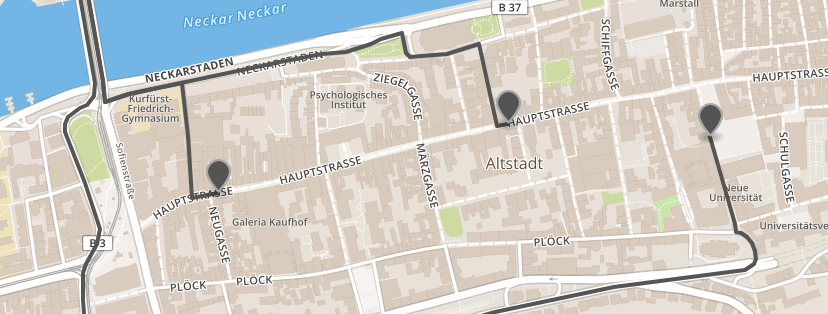
\includegraphics[width = 0.95\textwidth]{../media/Altstadt_emergency.png} \\
\caption{Emergency Routing}
\label{fig:alteme}
\end{subfigure}
\begin{subfigure}{0.49\textwidth}
\centering
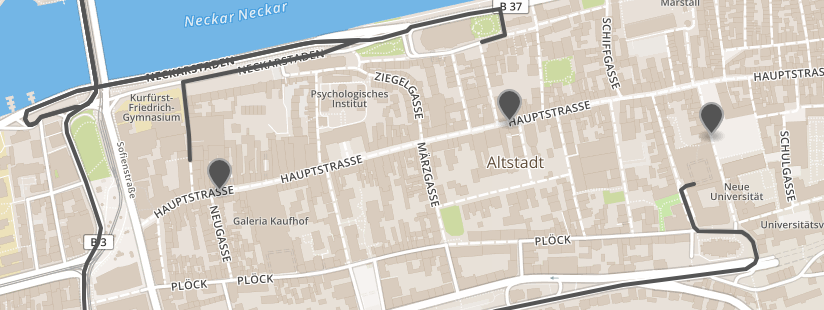
\includegraphics[width = 0.95\textwidth]{../media/Altstadt_car.png} \\
\caption{ORS-Car Routing}
\label{fig:altcar}
\end{subfigure}
\end{figure}

Im Folgenden wurden Isochronen mit der Freiwilligen Feuerwehr Gablingen als Zentrum berechnet (48.454063,10.824415 [Latitude, Longitude]). Folgende Einstellungen wurden dabei vorgenommen:

- Distanz: 5 min
- Intervall: 1 min
- Maximale Geschwindigkeit: 80 km/h für Löschfahrzeug und HGV; 130 km/h für PKW und Einsatzfahrzeug
- HGV Einstellungen für Löschfahrzeug und HGV: Länge=7m ; Breite= 2.5m; Höhe= 3m; Gewicht= 7.5t

Die Ersten Ergebnisse lieferten zu erwartende Resultate \ref{fig:isochrones}. Die Emergency Profile konnten in der gleichen Zeit einen größeren Bereich abdecken.

\begin{figure}[h]
\centering
\begin{subfigure}{0.49\textwidth}
\centering
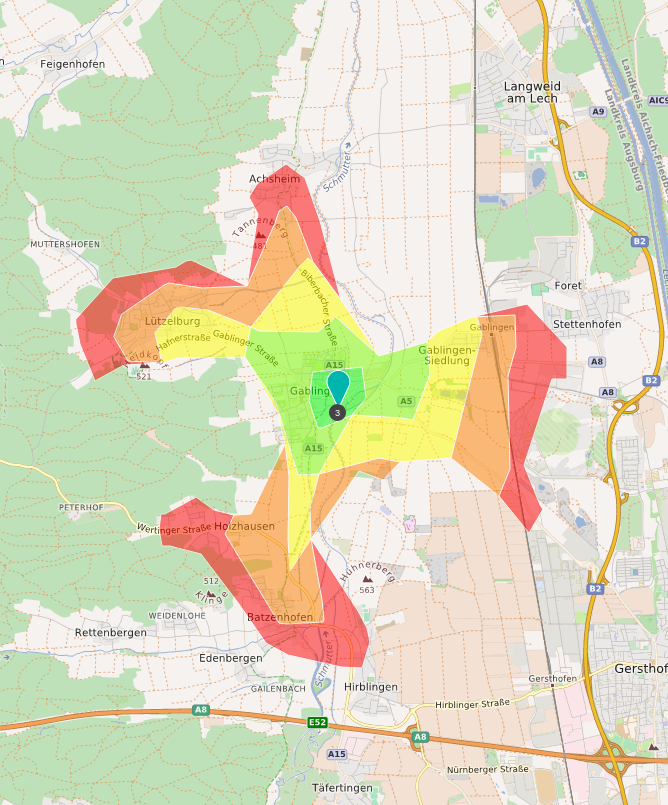
\includegraphics[width = 0.75\textwidth]{../media/isohgv.png} \\
\caption{HGV-Profil}
\label{fig:isohgv}
\end{subfigure}
\begin{subfigure}{0.49\textwidth}
\centering
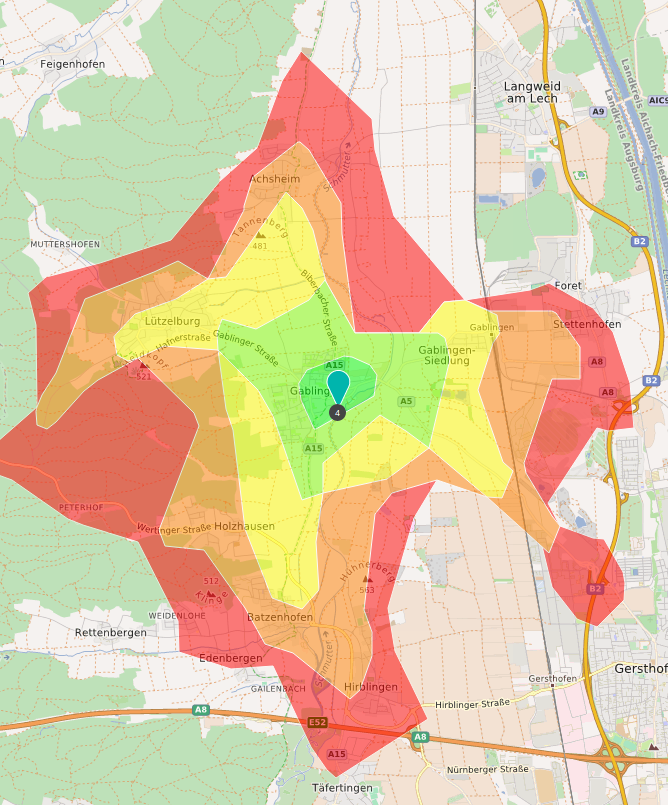
\includegraphics[width = 0.75\textwidth]{../media/isocar.png} \\
\caption{Car-Profil}
\label{fig:isocar}
\end{subfigure}
\begin{subfigure}{0.49\textwidth}
\centering
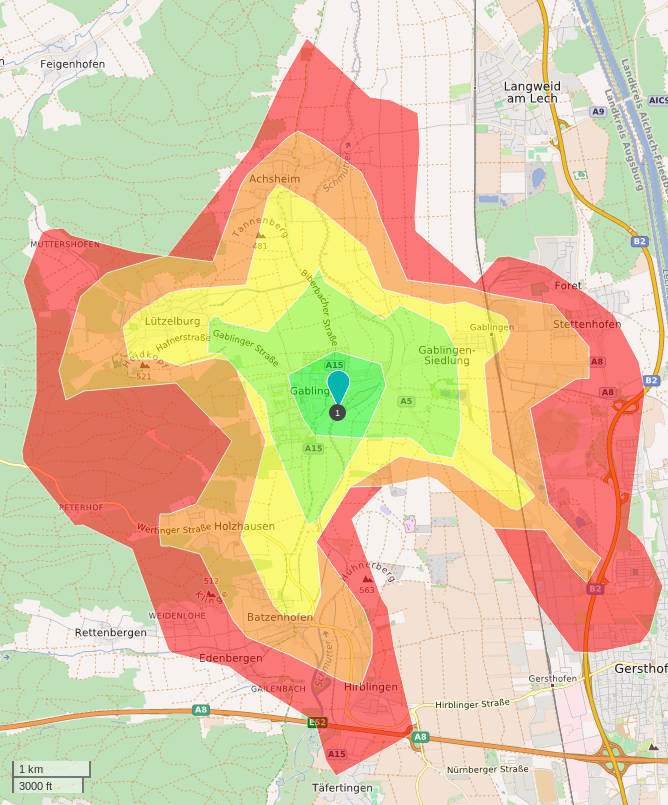
\includegraphics[width = 0.75\textwidth]{../media/isofire.png} \\
\caption{Emergency-Profil -- Löschfahrzeug}
\label{fig:isofire}
\end{subfigure}
\begin{subfigure}{0.49\textwidth}
\centering
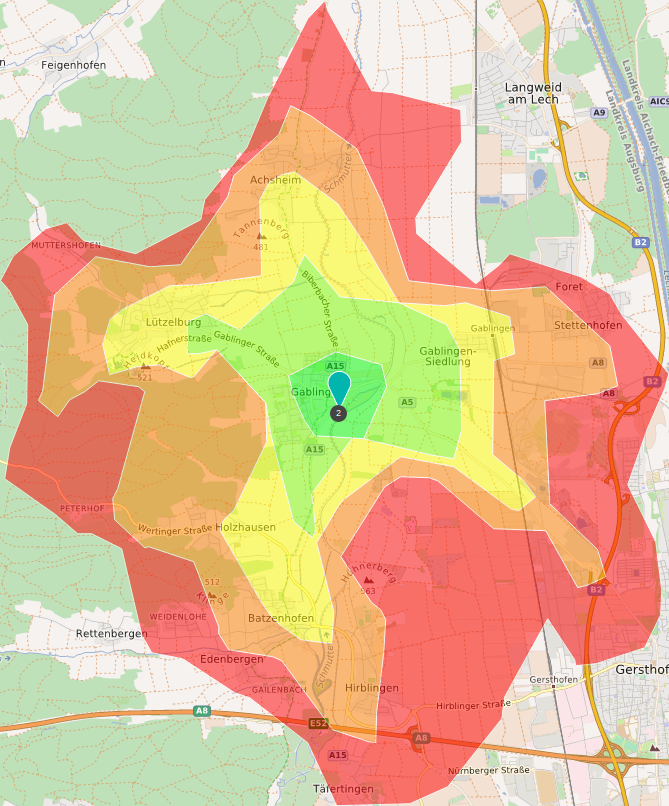
\includegraphics[width = 0.75\textwidth]{../media/isoeme.png} \\
\caption{Emergency-Profil -- Einsatzfahrzeug}
\label{fig:isoeme}
\end{subfigure}
\begin{subfigure}{0.90\textwidth}
\centering

\includegraphics[width = 0.75\textwidth]{../media/legendiso.png} \\
\end{subfigure}
\caption{Ergebnis Isochronen}
\label{fig:isochrones}
\end{figure}

\todo{
mehr blabla
+ bilder isos 
erreichbarkeits gebiet tabelle ?
eingehen auf eingeschlossene gebiete (keine löcher durch alpha shapes!)?
}

Nach einer Testfahrt der FFL wurde allerdings schnell klar, dass die Ergebnisse nicht im realistischen Bereich liegen. In fünf Minuten konnte das Löschfahrzeug auf der Einsatzfahrt vom Startpunkt in Gablingen Richtung Muttershofen nur den nordwestlichen Rand von Lützelburg erreichen. Das Profil kam für das Löschfahrzeug sogar über Muttershofen hinaus.



Um genaue Anpassungen am Backend vorzunehmen wurde eine weitere Testfahrt durchgeführt, bei der für jede volle Minute der Aufenthaltsort des Fahrzeuges markiert wurde (Abb. \ref{fig:drive1}).
Diese Angaben wurden mit den bisherigen Rückgabewerten des Profils verglichen.
Wie aus der Gesamtdauer für die Strecke in Tabelle \ref{tab:driveinit} ersichtlich, ist das Emergency Profil ungefähr 90 Sekunden zu schnell.

\begin{figure}[h]
\centering
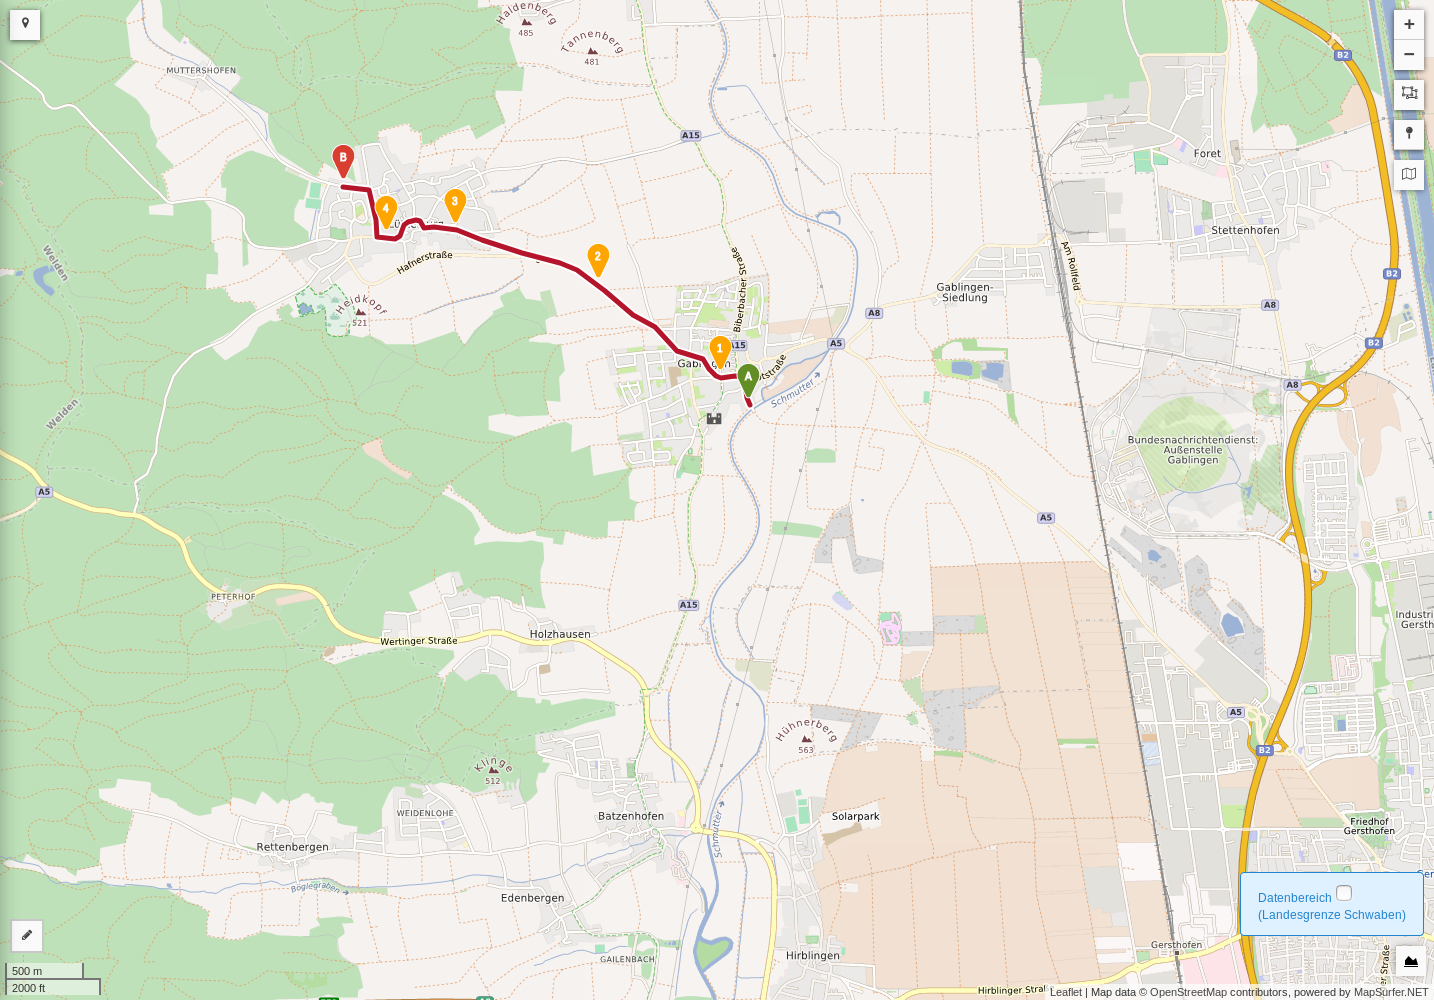
\includegraphics[width = 0.7 \textwidth]{../media/Fahrt1.png} \\
\caption{Testfahrt 1}
\label{fig:drive1}
\end{figure}

\begin{table}[]
\centering
\caption{Fahrt 1 -- 1. Auswertung}
\label{tab:driveinit}
\begin{tabular}{|l|r|r|r|r|r|}
\hline
Wegpunkt                               & \multicolumn{1}{c|}{1} & \multicolumn{1}{c|}{2} & \multicolumn{1}{c|}{3} & \multicolumn{1}{c|}{4} & \multicolumn{1}{c|}{B}  \\ \hline
Distanz                                & 363,2 m                & 1352,8 m               & 2331,9 m               & 2862,3 m               & 3387,3 m               \\ \hline
Fahrtzeit (Profil)                     & 28,6 s                 & 88,7 s                 & 139,4 s                & 177,6 s                & 209,8 s                \\ \hline
Fahrtzeit (Testfahrt)                  & 60,0 s                 & 120,0 s                & 180,0 s                & 240,0 s                & 300,0 s                \\ \hline
Fahrtzeit Abschnitt                    & 28,6 s                 & 60,1 s                 & 50,7 s                 & 38,2 s                 & 32,2 s                 \\ \hline
Fahrtzeit Abschnitt (Testfahrt)        & 60,0 s                 & 60,0 s                 & 60,0 s                 & 60,0 s                 & 60,0 s                 \\ \hline
Geschwindigkeit                        & 45,7 km/h              & 59,3 km/h              & 69,5 km/h              & 50,0 km/h              & 58,7 km/h              \\ \hline
Geschwindigkeit (Testfahrt)            & 21,8 km/h              & 59,4 km/h              & 58,7 km/h              & 31,8 km/h              & 31,5 km/h              \\ \hline
\end{tabular}
\end{table}

Die Vermutung liegt nahe, dass die große Differenz aufgrund der fehlenden Beschleunigungs- und Bremszeiten auftritt. Bisher wird von graphhopper bei der Berechnung der Fahrzeit lediglich 90$\%$ des für ein Segment vorgegebenen Geschwindigkeitslimits verwendet. Damit soll sichergestellt sein, dass die Geschwindigkeitsbegrenzung auf jedenfall eingehalten wird. Dieser Faktor wurde für das Emergency Profil entfernt.
Es wird also ein Straßensegment auf dem 50 km/h gefahren werden darf über die komplette Distanz bisher auch mit 50 km/h gefahren.
In der Realität braucht ein Fahrzeug dieser Größenordnung aber einige Sekunden um diese Geschwindigkeit aus dem Stand zu erreichen. Die selbe Situation besteht für Bremsvorgänge.
Es bestehen also drei Szenarien auf einer Fahrt, welche nach festgelegter Route einen Einfluss auf die Fahrzeit haben. Das sind der Start, ein Abbiegevorgang (engl.: Turn) und die Ankunft. Es gibt selbstverständlich noch mehr Faktoren die zum Beispiel andere Verkehrsteilnehmer betreffen, aber die drei genannten Szenarien sind bereits aus der Routenführung ersichtlich und werden definitiv bei jeder Fahrt auftreten\footnote{Wenn die Fahrt nur geradeaus geht ist auch kein Abbiegevorgang dabei}.

Anhand dieser Idee wurde eine weitere Java-Klasse \texttt{AccelerationWeighting} in der die zusätzliche Zeit für diese Szenarien berechnet wird implementiert (\ref{sec:anhang}).
Diese Klasse soll zwei Funktionen erfüllen. Zum einen muss bereits bei der Suche nach dem schnellsten Weg im Gegensatz zu geraden Strecken zusätzliche Zeit für Turns mit einfließen. Zum Anderen müssen bei der Berechnung der Fahrzeit Start-, Ankunfts- und Turnzeit mit berücksichtigt werden. 
Es stellt sich die Frage, wie eine Turn auf dem Graphen identifiziert werden kann. Die Änderung des Straßennamens ist sicherlich eine Möglichkeit viele Abbiegevorgänge abzudecken. Allerdings ist nicht immer ein Straßenname vorhanden und nicht immer bedeutet der Wechsel des Straßennamens, dass in diese Straße eingebogen werden muss.
Eine bessere Lösung bietet die Ausrichtung der Straßensegmente, da hier die Daten auf jeden Fall vorhanden sind. Deshalb wird in der AccelerationWeighting Klasse an Tower Nodes (also Kreuzungen) der Winkel zwischen dem letzten und dem nächsten Straßensegment berechnet.
Eine Abbiegung bzw. scharfe Kurve wird durch einen Winkel zwischen 50 und 140 Grad definiert.
Bei einer Routing Abfrage wird in einem solchen Fall das Gewicht der auf die Kurve folgenden Kante erhöht. Ebenso wird sobald der schnellste Weg ermittelt ist an diesen Stellen die Bremszeit vor der Abbiegung und die Beschleunigungszeit nach der Abbiegung zur Gesamtzeit des folgenden Wegsegmentes addiert. Der gleiche Vorgang wird für Start und Ziel durchgeführt. Die addierte Zeit wird als \textit{Penalty} (dt.: Strafe) bezeichnet.

Anhand der vorliegenden Testfahrt wurde das Profil derart kalibriert, dass durch die Penalties für Abbiegungen, Start und Ziel genau die fehlenden 90 Sekunden gebraucht wurden.
Für Start sowie Ankunft wurden 15 und für Abbiegungen 20 Sekunden veranschlagt.

Mit dem neu eingestellten Profil wurde nun erneut ein Request für die erste Testfahrt gesendet. Wie erwarte brauchte das Profil nun für diesen Weg ebenfalls fast genau fünf Minuten.
In Tabelle \ref{tab:drive11} ist die Differenz zu den einzelnen Minutenmarkern der 1. Testfahrt für diesen Request zu sehen. Diese Ergebnisse zeigen dass das Profil den ersten Teil der Route zu langsam und den zweiten Teil zu schnell absolviert.

\begin{table}[h]
\centering
\caption{Fahrt 1 -- Fahrzeit}
\label{tab:drive11}
\begin{tabular}{|l|r|r|}
\hline
Wegpunkt & Fahrtzeit & Abweichung \\ \hline 
1min & 78,3 s & $+18,3$ \\
2min & 138.5 s & $+18,5$ \\
3min & 188.5 s & $+8,5$ \\
4min & 226.7 s & $-3,3$ \\
5min & 298.9 s & $-1,1$ \\
\hline
\end{tabular}
\end{table}

Diese Kalibrierung wurde an zwei weiteren Testfahrten (Abb. \ref{fig:drive2} und \ref{fig:drive3}) vom selben Ausgangspunkt überprüft.

In den Tabellen \ref{tab:drive2} und \ref{tab:drive3} ist zu sehen, das 8 von 10 Wegpunkten um mehr als 20 Sekunden, in 3 Fällen sogar 40 Sekunden zu spät erreicht werden.
Mit den Ergebnissen dieser Testfahrten steht fest: das Profil ist noch erheblich zu langsam und die Penalties zu hoch.

\begin{figure}[h]
\centering
\caption{Testfahrt 2}
\label{fig:drive2}
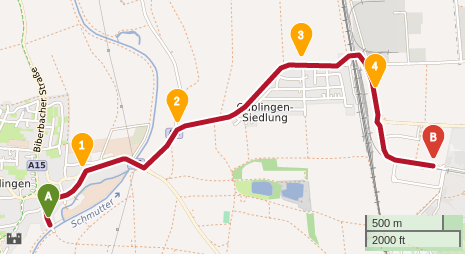
\includegraphics[width = 0.70 \textwidth]{../media/Fahrt2crop.png} \\
\end{figure}

\begin{table}[]
\centering
\caption{Fahrt 2 -- Fahrzeit}
\label{tab:drive2}
\begin{tabular}{|l|r|r|}
\hline
Wegpunkt & Fahrtzeit & Abweichung \\ \hline 
1min & 86.6 $s$ & $+26.6 s$ \\
2min & 149.9 $s$ & $+29.9 s$ \\
3min & 207.5 $s$ & $+27.5 s$ \\
4min & 253.5 $s$ & $+13.5 s$ \\
5min & 318.6 $s$ & $+18.6 s$ \\
\hline
\end{tabular}
\end{table}


\begin{figure}[h]
\centering
\caption{Testfahrt 3}
\label{fig:drive3}
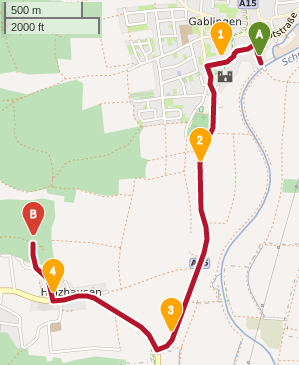
\includegraphics[width = 0.40 \textwidth]{../media/Fahrt3crop.png} \\
\end{figure}

\begin{table}[]
\centering
\caption{Fahrt 3 -- Fahrzeit}
\label{tab:drive3}
\begin{tabular}{|l|r|r|}
\hline
Wegpunkt & Fahrtzeit & Abweichung \\ \hline 
1min: &  89.8 s & $+29.8s$ \\
2min: &  162.4 s & $+42.4$ \\
3min: &  213 s & $+33$ \\
4min: &  282.3 s & $+42.3$ \\
5min: &  343.9 s & $+43.9$ \\
\hline
\end{tabular}
\end{table}

Die Penalties für Start und Ankunft wurden für die folgenden Analysen um die Hälfte reduziert und lagen somit bei 7,5 Sekunden. Turnpenalties wurden auf 16 Sekunden reduziert. 

Mit der neuen Gewichtung wurden die Requests für die drei Testfahrten erneut gesendet und mit den Minuten-Markierungen der wirklich benötigten Zeiten verglichen.
Die Ergebnisse sind der Tabelle \ref{tab:all} zu entnehmen.

\begin{table}[]
\centering
\caption{Fahrt 1,2,3 -- 2. Auswertung}
\label{tab:all}
\begin{tabular}{|l|r|r|r|r|r|r|}
\hhline{~|-|-|-|-|-|-}
\multicolumn{1}{l|}{} & \multicolumn{2}{c|}{Fahrt 1} & \multicolumn{2}{c|}{Fahrt 2} & \multicolumn{2}{c|}{Fahrt 3} \\ \hline
Wegpunkt & Fahrtzeit & Abweichung & Fahrtzeit & Abweichung & Fahrtzeit & Abweichung \\ \hline 
1min & 59.5 & -0.5 & 67.6 & +7.6 & 70.8 & +10.8  \\
2min & 119.5 & -0.5 & 126.9 & +6.9 & 139.4 & +19.4  \\
3min & 169.5 & -10.5 & 184.5 & +4.5 & 190 & +10  \\
4min & 207.7 & -32.2 & 230.5 & -10.5 & 255.2 & +15.2  \\
5min & 271.9 & -28.1 & 291.6 & -8.4 & 312.9 & +12.9   \\
\hline
\end{tabular}
\end{table}


Um die Testfahrten genauer analysieren zu können, wurde das Backend um bisher fehlende Funktionen für die Rückgabe von zusätzlichen Informationen. Dabei wurden die Speicherobjekte für Wegtypen und Wegoberfläche hinzugefügt und zusätzlich die Höheninformationen der Punte zurückgegeben. Im Frontend konnten dadurch nun die Wegtypen und Wegoberfächen aber auch die Steigung und somit auch ein Höhenprofil angezeigt werden. Außerdem wurde ein Feature zur Darstellung der Höchstgeschwindigkeit der einzelnen Streckensegmente eingebaut. 

\newpage

\section{Diskussion}

\subsection{Teststrecke 1}

Durch die implementierten Funktionen wurde ersichtlich, dass bei der Berechnung der Zeit bisher die Steigung als entscheidender Faktor nicht betrachtet wurde.
Auf der ersten Teststrecke muss das Löschfahrzeug insgesamt einen Höhenunterschied von ungefähr 70 Metern überwinden (Abb. \ref{profile}).
Über die Hälfte der Distanz hat dabei eine Steigung von 1-3$\%$ und auf einem Viertel der Strecke sogar eine Steigung von 4-6$\%$.
Ein Fahrzeug dieser Gewichtsklasse kann auf dieser Strecke folglich nicht die für den größten Teil dieses Anstiegs geltende Maximalgeschwindigkeit von 80 km/h erreichen.


\begin{figure}[htb]
\centering
\begin{subfigure}{0.80\textwidth}
\centering
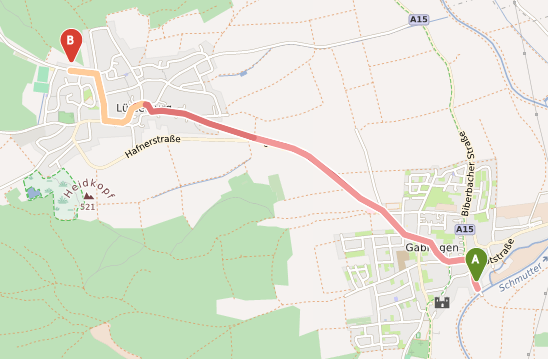
\includegraphics[width = \textwidth]{../media/Fahrt1_Steep.png} \\
\caption{Strecke 1 mit Steigung}
\label{fig:steig}
\end{subfigure}


\includegraphics[width =0.25 \textwidth]{../media/legend2.png} \\

\begin{subfigure}{ \textwidth}
\centering
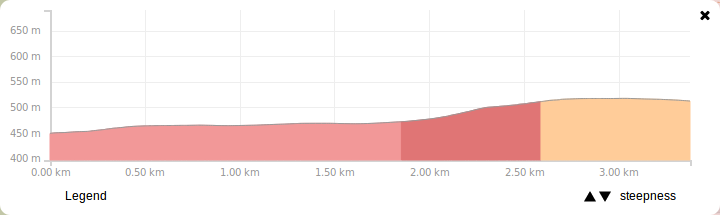
\includegraphics[width = \textwidth]{../media/Fahrt1_Profile.png} \\
\caption{Höhenprofil der ersten Strecke}
\label{profile}
\end{subfigure}
\caption{Fahrt 1 -- Steigung und Höhenprofil}
\label{steig}
\end{figure}

Darüber hinaus liegen auf der Strecke im inneren Lützelburgs einige langgezogene aber dennoch enge Kurven (Abb.~\ref{fig:curve}).
Auch hier kann das Löschfahrzeug nicht die gegebene Geschwindigkeit beibehalten und muss abbremsen.
Diese Kurven werden allerdings von Löschfahrzeug-Profil nicht als Abbiegung erkannt, da der Winkel zwischen den Segmenten zu groß ist.
Daher absolviert das Profil diesen Streckenabschnitt in geringerer Zeit als das echte Fahrzeug.

\begin{figure}[htb]
\centering
\caption{Fahrt 1 -- Unregistrierte Abbiegungen}
\label{fig:curve}
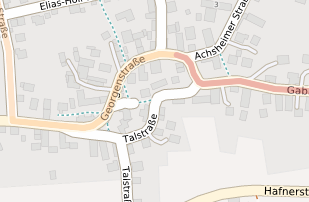
\includegraphics[width = 0.50 \textwidth]{../media/Fahrt1_curve.png} \\
\end{figure}

Weiterhin wurde für jede der drei Fahrten beobachtet, dass auf den Segmenten mit Maximalgeschwindigkeit (80 km/h) das Profil ebenfalls konstant ein paar Sekunden gegenüber der Testfahrt gutmachen kann.
Die Erklärung dafür ist, dass das Löschfahrzeug die angegebene Maximalgeschwindigkeit nicht komplett erreichen kann.
Auch wenn die Angabe mit der Geschwindigkeitsanzeige übereinstimmt, ist die effektive Geschwindigkeit geringer.

Die Zeitdifferenzen aus Tabelle \ref{tab:all} zeigen: das Profil fährt dem echten Fahrzeug mit der derzeitigen Gewichtung über die ganze Strecke hinweg.
Wenn die genannten Faktoren der Steigung, der nicht mit einberechneten schärferen Kurven und der Maximalgeschwindigkeit mit einbezogen werden, ist ein Ergebnis von etwa 5 Minuten zu erwarten.

\subsection{Teststrecke 2}

Da die 2. Strecke nur in der Ebene verläuft, sind keine Abweichungen durch die Steigung zu erwarten.
Die Differenzzeiten betragen für alle fünf Wegpunkte ungefähr 10 Sekunden.
Auffallend ist der Sprung vom 3. zum 4. Wegpunkt, bei welchem das Profil 14 Sekunden aufholt.
Nach einer genaueren Betrachtung dieses Segments stellte sich heraus, dass hier eine einspurige Unterführung durchfahren werden musste auf die eine durch die Topologie unübersichtliche Kurve folgt (Abb. \ref{fig:traintunnel}).
Daher kam es auf der Fahrt zu Verzögerungen, welches das Aufholen des Profils gegenüber der Testfahrt erklärt.

\begin{figure}[htb]
\centering
\caption{Fahrt 2 -- Unterführung}
\label{fig:traintunnel}
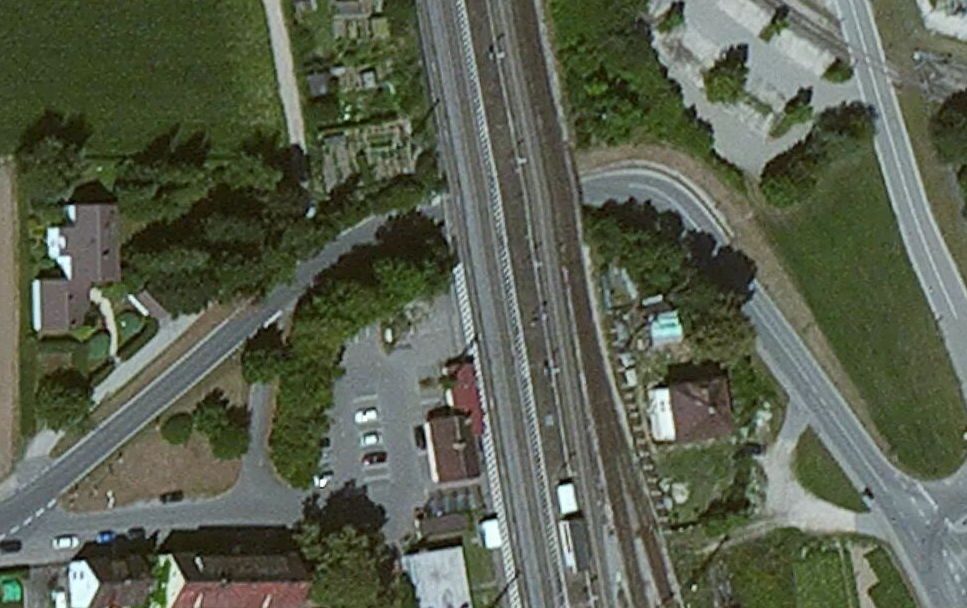
\includegraphics[width = 0.70 \textwidth]{../media/traintunnel.png} \\
\end{figure}


\subsection{Teststrecke 3}

Bei den Ergebnissen der 3. Strecke (Tab. \ref{tab:all}) ist das Profil bereits nach dem ersten Wegpunkt um mehr als 10 Sekunden zu langsam.
Bis zum Zwei-Minuten-Wegpunkt wird dieser Rückstand fast verdoppelt.
Nach genauerer Überprüfung der Durchschnittsgeschwindigkeiten stellte sich heraus, dass der Weg hier durch eine 30er-Zone führt.
Allerdings wird diese nicht mit den erwarteten 50 km/h sondern nur mit den durch den \texttt{maxspeed} Tag festgelegten 30 km/h durchfahren.
Offensichtlich ist dies ein Fehler im Backend welcher behoben werden muss.

\begin{figure}[htb]
\centering
\caption{Fahrt 3 -- Tempo-30-Zone}
\label{fig:temp30}
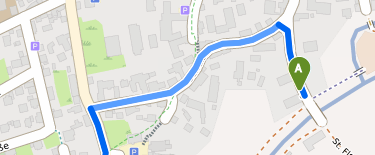
\includegraphics[width = 0.60 \textwidth]{../media/Fahrt3_temp30.png} \\

\includegraphics[width = 0.20 \textwidth]{../media/legend3.png} \\
\end{figure}

Die anfängliche 30er-Zone ist fast 350m lang.
Diese Strecke kann mit 50 km/h in 25,2 Sekunden und mit 30 km/h in 42 Sekunden durchfahren werden.
Wird die Differenz von 16.8 Sekunden von den bisherigen Abweichungen für die 3. Fahrt abgezogen, werden die neuen Werte aus Tabelle \ref{tab:new3} erhalten.

\begin{table}[htb]
\centering
\caption{Fahrt 3 -- neue Fahrzeit}
\label{tab:new3}
\begin{tabular}{|l|r|r|}
\hline
Wegpunkt & Fahrzeit & Abweichung \\ \hline 
1$min$ & 58.2$s$\footnote{Zum ersten Wegpunkt beträgt die Strecke nur 260m weshalb hier nur 12.6 Sekunden abgezogen werden} & -1.8$s$  \\
2$min$ & 122.6$s$ & +2.6$s$  \\
3$min$ & 173.2$s$ & -6.8$s$  \\
4$min$ & 238.4$s$ & -1.6$s$  \\
5$min$ & 296.1$s$ & -3.9$s$  \\
\hline
\end{tabular}
\end{table}

Vor der 2-Minuten-Marke beginnt eine Überlandstraße, die bis kurz vor Holzhausen (zwischen Marker 3 und 4) reicht.
Das sind 56$\%$ der Gesamtstrecke.
Wie bei der Diskussion der 1. Fahrt bereits erwähnt, ist zu erwarten, dass die Maximalgeschwindigkeit von 80km/h zu hoch angesetzt ist, welches den leichten Vorsprung zur 3-Minuten-Marke erklärt.

\begin{figure}[htb]
\centering
\begin{subfigure}{0.49\textwidth}
\centering
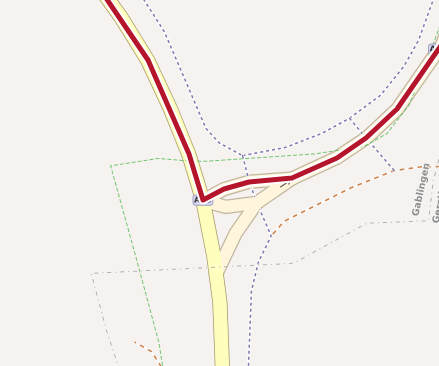
\includegraphics[width = 0.80\textwidth]{../media/Fahrt3_Turn.png} \\
\caption{Abbiegung auf \gls{osm}-Datenebene}
\label{fig:turnosm}
\end{subfigure}
\begin{subfigure}{0.49\textwidth}
\centering
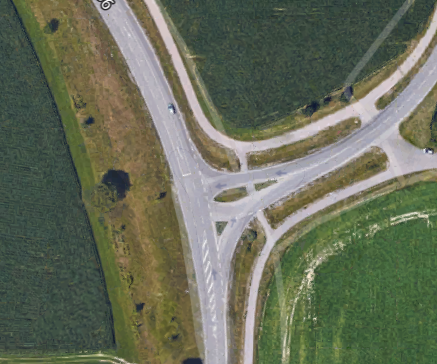
\includegraphics[width = 0.80\textwidth]{../media/Fahrt3_actualturn.png} \\
\caption{Eigentliche Abbiegung}
\label{fig:turnworld}
\end{subfigure}
\caption{Fahrt 3 -- Vergleich eines Abbiegevorgangs}
\label{fig:turn}
\end{figure}

Zwischen Punkt 3 und 4 fällt das Löschfahrzeug-Profil um fünf Sekunden zurück.
Zwischen diesen Punkten befindet sich eine Abbiegung, die deutlich schneller als andere Kurven gefahren werden kann.
Abbildung \ref{fig:turn} zeigt einen Vergleich dieses Abbiegevorgangs zwischen den \gls{osm} Daten(\ref{fig:turnosm}) und der eigentlichen Straße(\ref{fig:turnworld}).
Es ist zu erkennen, dass die Abbiegung um einiges ''weicher'' ist als die Daten beschreiben.
Daher konnte das Löschfahrzeug gegenüber dem Profil hier Zeit gewinnen.

Schließlich zeigte auch diese Strecke nach einer Untersuchung des Höhenprofils einen Anstieg auf den letzten 150 Metern um 7-9$\%$(Abb. \ref{fig:profile2}), der noch nicht mit einberechnet wird, und dem Löschfahrzeug-Profil somit einen kleinen Vorsprung gibt.

\begin{figure}[htb]
\centering
\caption{Fahrt 3 -- Höhenprofil}
\label{fig:profile2}
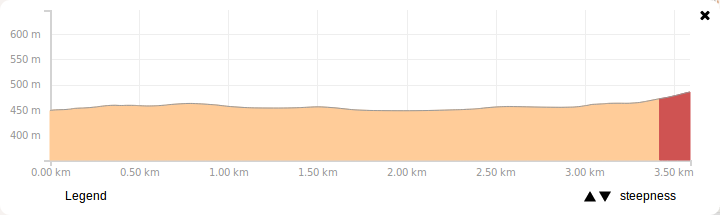
\includegraphics[width = 0.90 \textwidth]{../media/Fahrt3_Profile.png} \\
\end{figure}


\subsection{Benötigte Änderungen}

Wie durch die vorliegenden Analysen zu sehen ist, müssen einige Änderungen vollzogen werden, damit das Profil realistischere Ergebnisse zurückgibt.\par
\begin{itemize}
\item 30er Zonen werden noch nicht richtig erkannt.
\item Die Steigung muss berücksichtigt werden.
\item Abbiegevorgänge innerhalb von Segmenten (Abb.~\ref{fig:curve}), an Pillar Nodes, werden bisher nicht berücksichtigt und müssen mit einbezogen werden.
\item Die Zeit für einen Abbiegevorgang sollte sowohl anhand des effektiven Winkels als auch anhand der Geschwindigkeiten des vorherigen und folgenden Wegsegmentes bestimmt werden.
Ansätze hierfür wurden bereits entwickelt (siehe Source Code), wurden allerdings noch nicht getestet.
\item Für die Penalties muss die Zeit, sofern vorhanden, aus der eigentlichen Beschleunigung und falls diese nicht vorhanden, zum Beispiel aus dem Gewicht des Fahrzeugs berechnet werden.
Dadurch können einfacher spezifische Fahrzeugprofile erstellt und getestet werden.
Da das \texttt{AccelerationWeighting} sowohl für das Löschfahrzeug als auch für allgemeine Einsatzfahrzeuge benutzt wird, erhalten diese bisher die gleichen Penalties.
\item Weiterhin muss für Einbahnstraßen, die in Gegenrichtung durchfahren werden, ein Penalty (ca. *0.9) gesetzt werden, da diese oft nicht mit der selben Geschwindigkeit durchfahren werden können, wie in der eigentlichen Fahrtrichtung (auch wenn es erlaubt ist).
Auf diese Weise kann außerdem ein Routing auf der Gegenfahrbahn, lediglich für den Gewinn von wenigen Sekunden, verhindert werden.
Darüber hinaus werden damit bevorzugt vorhandene Parallelstraßen benutzt.
\end{itemize}

\newpage

\section{Fazit}

Das erstellte Profil für Löschfahrzeuge wird als Prototyp betrachtet und kann bereits die Grundlegenden geforderten Eigenschaften erfüllen.
Es werden bei der Suche nach dem kürzesten Weg in einem Straßennetz die für andere Fahrzeuge geltenden Geschwindigkeitslimits auf geeignetere Werte angehoben.

Es ist für das Profil möglich Einbahnstraßen in Beide Richtungen zu durchfahren.
Bisher wird deswegen allerdings ab und zu die Gegenfahrbahn über längere Distanzen wegen einem Gewinn von nur wenigen Sekunden verwendet.
Darüber hinaus würde ein Penalty dem Risiko des Gegenverkehrs gerecht werden.
Interessant wäre es daher einen Penalty-Faktor einzubauen, der bei einer Nutzung entgegen der Fahrtrichtung eine Verzögerung mit einberechnet.
Dadurch würden auch in der Nähe liegende Parallelstraßen vorgezogen werden.
Darüber hinaus werden bisher nicht befahrbare Straßentypen wie Fußgängerzonen und Radwege für das Profil verfügbar gemacht.
Eine Routenführung bis zum Zielpunkt wird so gegenüber den normalen Fahrzeug Profilen in den meisten Fällen erreicht.

Derzeit wird die Schwerfälligkeit des Löschfahrzeuges durch positive Faktorisierung\footnote{Die Gewichtung wird mit Werten größer 1.0 multipliziert} der Gewichtung für Start, Ankunft und Turns bei der Suche nach dem schnellsten Weg berücksichtigt.
Für die durchgeführten Teststrecken wurde beim routen von Start bis Endpunkt jeweils genau die richtige Route zurückgegeben.
Ob diese Faktorisierung allgemein gültig ist, muss noch durch weitere Analysen überprüft werden.
Für die Berechnung der Zeit werden zur Berücksichtigung der Schwerfälligkeit einfache Penalties für Start, Ankunft und Turns verwendet.
Hierbei wird ein Turn durch den Winkel zwischen zwei Straßensegmenten an einer Kreuzung ermittelt.
Bisher erhält jeder Turn den gleichen Penalty obwohl manche Kurven schneller gefahren werden können.
Kurven innerhalb eines Segmentes werden bisher noch nicht registriert.

Für realistischere Ergebnisse müssen diese Kurven ebenfalls als Turn registriert werden.
Darüber hinaus muss der Öffnungswinkel einer Kurve mit in die Berechnung der zusätzlichen Zeit einfließen, da Turns mit größerem Winkel auch schneller gefahren werden können.
Gleichzeitig muss auch die Geschwindigkeit des vorherigen und folgenden Straßensegments beachtet werden, da diese die Brems- bzw. Beschleunigungsstrecke alterieren.
Die Steigung eines Straßensegments hat einen signifikannten Einfluss auf die benötigte Zeit und muss daher ebenfalls einkalkuliert werden.
Es werden für die Implementierung dieser Funktionen noch weitere Analysen zu speziellen Testfahren für das jeweilige Szenario (Steigung, Turn) benötigt.

Die Fahrzeugdimensionen und die Höchstgeschwindigkeit sind nicht im Backend festcodiert sondern können als Parameter bei der Abfrage mitgeliefert werden.
Damit ist eine Erweiterung für andere Fahrzeugklassen der Feuerwehr als auch des Rettungsdienstes oder der Polizei möglich, da für alle die selbe Grundprämisse gilt (~\ref{cit:STVO}).

Im Hinblick auf \gls{osm}-Daten kann keine endgültige Sicherheit gewährleistet werden, da die Ergebnisse höchstens so gut wie die Daten sein können

Für die Erstellung von Einzugsgebieten für das Emergency Profil, muss letztlich die Gewichtung für den Isochrones Service verfügbar gemacht werden.
Das ist in der bisherigen Implementierung noch nicht gelungen.

\newpage
\section{Ausblick}

\todo{Add Ausblick to Fazit?}

Das Analysieren der Teststrecken ist durch das einzelne Senden der Requests und das anschließende Extrahieren der benötigten Werte relativ zeitaufwändig.
Es wäre hilfreich ein Werkzeug zum gleichzeitigen senden von allen Testrequests zu entwickeln mit welchem danach ebenso die Antworten adäquat dargestellt werden können.
Dabei sollten zum Beispiel die Distanzen zwischen wichtigen Änderungspunkten auf einer Route berechnet werden können und direkt Tabellarisch aufgelistet werden.

Ein weiterer interessanter Aspekt den es zu beleuchten gilt, ist das unterschiedliche Verkehrsaufkommen auf einer Straße oder Fußgängerzone.
So könnten Geschwindigkeiten für bestimmte Wegsegmente je nach Zeit anhand von Berufsverkehr oder Tageszeit angepasst werden.
Nachts sollten zum Beispiel generell weniger Autos unterwegs sein, wodurch Zeit gespaart wird, Umgekehrt zur Rush-Hour.

Die im Fragebogen erwähnte Suche nach Löschwasser Quellen am Zielort kann und sollte verwirklicht werden.
In der \gls{osm} Datengrundlage existieren bereits diverse Tags für Objekte die von Einsatzkräften genutzt werden können.
Für die Feuerwehr besonders interessant ist zum Beispiel der \texttt{emergency=fire\_hydrant} Tag für Hydranten.
In vielen Städten sind diese durch das OpenFireMap-Projekt\footnote{https://wiki.openstreetmap.org/wiki/DE:OpenFireMap} flächendeckend abdigitalisiert und der OSM Datenbank zugefügt worden (Abb.~\ref{fig:firehydrants}).

\begin{figure}[h]
\centering
\caption{Hydranten Informationen in Heidelberg}
\label{fig:firehydrants}
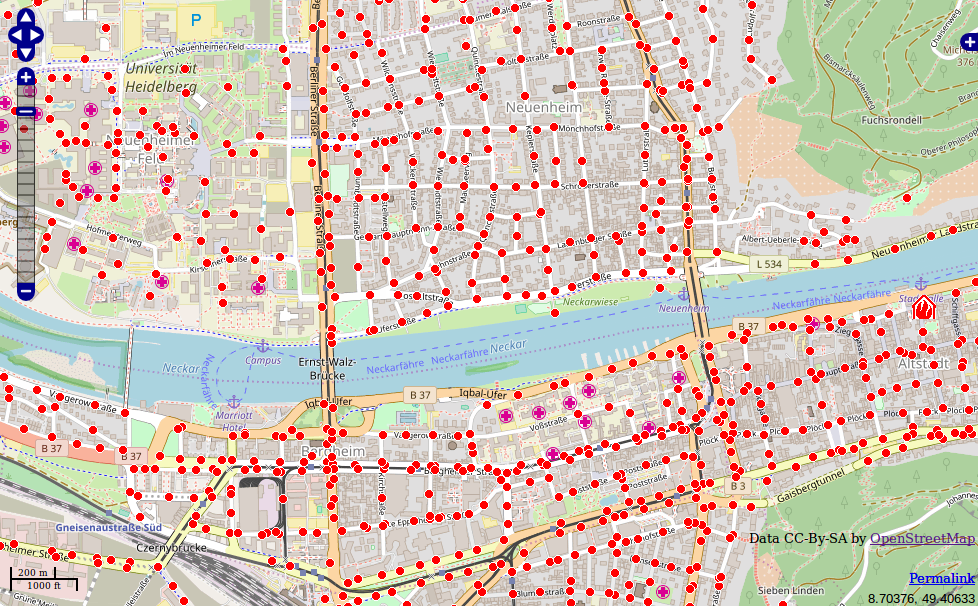
\includegraphics[width = 0.80 \textwidth]{../media/firehydrants.png} \\
\end{figure}


\newpage
\printbibliography
\addtocounter{section}{1}
\addcontentsline{toc}{section}{\protect\numberline{\thesection}Literatur}

\newpage



\section{Anhang}
\label{sec:anhang}
\subsection*{Copyrights}
Die Rechte für die mit geojson.io generierten Abbildungen(\ref{fig:footway}, \ref{fig:school}, \ref{fig:ramp}, \ref{fig:oneway}, \ref{fig:opposite}) gehen an \copyright Mapbox für den Kartenstil und \copyright OpenStreetMap für die Daten.
\newline Die Rechte der mit dem \gls{ors} entworfenen Abbildungen(\ref{fig:isochrones}, \ref{fig:drive1}, \ref{fig:drive2}, \ref{fig:drive3}, \ref{fig:steig}, \ref{fig:curve}, \ref{fig:temp30}, \ref{fig:turnosm}) gehen an \copyright OpenStreetMap contributors für die Daten und \copyright Maxim Rylov für den Kartenstil.
Für Abbildung \ref{fig:turnworld} liegt das Copyright bei \copyright 2017 Google für die Bilder und \copyright 2017 GeoBasis-DE/BKG für die Kartendaten.
Für Abbildung \ref{fig:traintunnel} liegt das Copyright bei \copyright DigitalGlobe.

\subsection*{Links}
\textbf{Fragenkatalog:}
\sloppy
\url{https://docs.google.com/document/d/1nwjmea0jwauJWezk\_2TMQs5CbAHv7he2NI4kxqMu2w4/}
\medskip

\textbf{Emergency Routing Service:}

\url{http://emergency.openrouteservice.org/directions?n1=48.448646\&n2=10.826855\&n3=14\&b=0\&c=0\&k1=en-US\&k2=km}
\medskip

\textbf{Testfahrt 1:}

GeoJson-Antwort:\par
\url{https://disaster-api.openrouteservice.org/emergency/routes?api_key=58d904a497c67e00015b45fcbd837ca3e137425f653e26a676ecd396&attributes=detourfactor|percentage&coordinates=10.824569,48.454111|10.789776,48.466555&elevation=true&extra_info=steepness|waytype|surface|avgspeed&geometry=true&geometry_format=geojson&instructions=true&instructions_format=html&language=en-US&options={"profile_params":{"restrictions":{"width":"2.5","height":"3","weight":"7.5","length":"7"}},"maximum_speed":"80"}\&preference=fastest\&profile=driving-emergency\&units=m}
\medskip

Anzeige im \gls{ors} Client:\par
\url{http://emergency.openrouteservice.org/directions?n1=48.454186&n2=10.825616&n3=18&a=48.454111,10.824569,48.466555,10.789776&b=5b&c=0&f3=3&f1=7.5&f2=2.5&f5=7&d=80&k1=en-US&k2=km}
\medskip

\textbf{Testfahrt 2:}

GeoJson-Antwort:\par
\url{https://disaster-api.openrouteservice.org/emergency/routes?api_key=58d904a497c67e00015b45fcbd837ca3e137425f653e26a676ecd396&attributes=detourfactor|percentage&coordinates=10.824569,48.454111|10.85755,48.457434&elevation=true&extra_info=steepness|waytype|surface|avgspeed&geometry=true&geometry_format=geojson&instructions=true&instructions_format=html&language=en-US&options={"profile_params":{"restrictions":{"width":"2.5","height":"3","weight":"7.5","length":"7"}},"maximum_speed":"80"}&preference=fastest\&profile=driving-emergency&units=m}
\medskip

Anzeige im \gls{ors} Client:\par
\url{http://emergency.openrouteservice.org/directions?n1=48.454236&n2=10.826409&n3=18&a=48.454111,10.824569,48.457434,10.85755&b=5b&c=0&d=80&f3=3&f1=7.5&f2=2.5&f5=7&k1=en-US&k2=km}
\medskip

\textbf{Testfahrt 3:}

GeoJson-Antwort:\par
\url{https://disaster-api.openrouteservice.org/emergency/routes?api_key=58d904a497c67e00015b45fcbd837ca3e137425f653e26a676ecd396&attributes=detourfactor|percentage&coordinates=10.824569,48.454111|10.805097,48.443849&elevation=true&extra_info=steepness|waytype|surface|avgspeed&geometry=true&geometry_format=geojson&instructions=true&instructions_format=html&language=en-US&options={"profile_params":{"restrictions":{"width":"2.5","height":"3","weight":"7.5","length":"7"}},"maximum_speed":"80"}&preference=fastest&profile=driving-emergency&units=m}
\medskip

Anzeige im \gls{ors} Client:\par
\url{http://emergency.openrouteservice.org/directions?n1=48.44654&n2=10.826383&n3=15&a=48.454111,10.824569,48.443849,10.805097&b=5b&c=0&d=80&f3=3&f1=7.5&f2=2.5&f5=7&k1=en-US&k2=km}
\medskip

\subsection*{Sourcecode}
\label{sec:source}

\sloppy
\textbf{Komplettes Backend:}\newline
\url{https://github.com/TheGreatRefrigerator/openrouteservice/tree/emergencyrouting}
\newline
\smallskip
\textbf{Erstellte Java-Klassen}\newline
\url{https://github.com/TheGreatRefrigerator/ba_thesis/tree/master/data/JavaFiles}
\newline
\medskip
\textbf{Frontend:}\newline
\url{https://github.com/GIScience/openrouteservice-app/tree/emergencyrouting}
\fussy

\newpage
\section*{Erklärung}
\vspace{1cm}
Hiermit versichere ich, dass ich die vorliegende Bachelorarbeit selbstständig verfasst, noch nicht anderweitig zu Prüfungszwecken vorgelegt, keine anderen als die angegebenen Quellen oder Hilfsmittel benutzt, sowie wörtlich und sinngemäße Zitate als solche gekennzeichnet habe.\par
\bigskip

{\flushleft Heidelberg den \today } {\hfill .....................................\par}
{\hfill (Unterschrift)}

\newpage
\section*{Danksagungen}

An dieser Stelle möchte ich allen Personen danken, die dazu beigetragen haben diese Arbeit zu verwirklichen.\par
\vspace{0.5cm}
Ein großes Dankeschön geht natürlich an die Freiwillige Feuerwehr Lützelburg für die Bereitstellung des Fahrzeuges.
Insbesondere möchte ich Stefan Witossek für die detaillierten Informationen sowie die Organisation und Durchführung aller Testfahrten danken.
Ohne ihn wäre diese Arbeit nicht möglich gewesen.\par
\vspace{0.5cm}
Danke an meine Kollegen vom Openrouteservice Team Timothy Ellersiek, Maximilian Rylov und Lu Liu, die mir mit motivierenden Gesprächen und hilfreichen Erklärungen zur Seite gestanden sind und mich in jeder Hinsicht unterstützt haben.\par
\vspace{0.5cm}
Bei meinem Betreuer Prof. Dr. Alexander Zipf möchte ich mich für das Prüfen der Arbeit und der Möglichkeit bedanken beim Openrouteservice zu arbeiten.\par
Ebenfalls bedanken möchte ich mich bei Prof. Dr. Jo\~ao Porto de Albuquerque, der trotz eines mit internationalen Reisen gefüllten Terminkalenders Zeit für das Prüfen meiner Arbeit gefunden hat.\par
\vspace{0.5cm}
Außerdem möchte ich mich bei meinen Kommilitonen Angelika Kinas und Marcel Reinmuth sowie meiner Freundin Nanni XY bedanken, die mich in dieser Zeit mit unterhaltsamen Mittagspausen, motivierenden Gesprächen, Tipps und dem Korrekturlesen der Arbeit besonders unterstützt haben.


\newpage
\vspace{1cm}
%last page


\end{document}
